%=======================+=========================
%================  Performance  ================
%=================================================

\section[Detector performance]{Detector performance \label{sec:performance}}                                                 

The capability of the \gx{} detector in reconstructing charged and neutral particles and assembling them into fully reconstructed events has been studied in data and simulation using several photoproduction reactions.  The results of these studies are summarized in this section.

%\subsection{Charged particles \label{sec:perfcharged}} 

%\subsubsection{Efficiency \label{sec:perfchargedeff}}

%The reconstruction efficiency for different hadron species has been studied using the method described in Sec.~\ref{sec:trackeff}.   Charged pion reconstruction efficiency was studied with a sample of $\gamma p \to p \omega$, $\omega \to \pi^+\pi^-\pi^0$ events.  Charged kaon reconstruction efficiency was studied with samples of $\gamma p \to \phi p$, $\phi \to K^+K^-$ and $\gamma p \to \Lambda(1520) K^+$, $\Lambda(1520) \to p K^-$ events.  Proton reconstruction efficiency was studied with a sample of $\gamma p \to K^+ \Sigma^0$, $\Sigma^0 \to \gamma \Lambda^0$, $\Lambda^0 \to p \pi^-$ events.  
%The results are illustrated in Fig.~X. The efficiencies determined by data and simulation generally agree to within a few percent.

\subsection{Charged-particle reconstruction efficiency  \label{sec:trackeff}}
The track reconstruction efficiency was estimated by analyzing $\gamma p \rightarrow p \omega$, $\omega\rightarrow\pi^+\pi^-\pi^0$ events, where the proton, the $\pi^0$, and one of the charged pions were used to predict the three-momentum of the other charged pion. Two methods were used to calculate this efficiency, $\varepsilon=N_{found}/(N_{found}+N_{missing})$.  Events for which no track was reconstructed in the predicted region of 
phase space contributed to $N_{missing}$, while events where the expected track was reconstructed contributed to $N_{found}$.  For the first method, the $\omega$ yields for $N_{found}$ and $N_{missing}$ were estimated from the missing mass off the 
proton; for the second method, the invariant mass of the $\pi^+\pi^-\pi^0$ system was used to find $N_{found}$.  This analysis was performed for individual bins of track momentum, $\theta$, and $\phi$.
Examples of mass histograms for a typical bin in $\phi$ are shown in Fig.~\ref{fig:omega mass}.  The exercise was repeated for a sample of $\omega$ Monte Carlo events.   A comparison of the efficiency for pion reconstruction derived from the 
two methods for both Monte Carlo and experimental data is shown in Fig.~\ref{fig:tracking efficiency}.  The efficiencies for Monte Carlo and experimental data 
agree to within 5\%.

While this reaction only allows the determination of track reconstruction efficiencies for $\theta < 30^\circ$, this covers the majority of charged particles produced in \gx{} due to its fixed-target geometry.  Other reactions are being studied to determine the efficiency at larger angles.

\begin{figure}[tbp]
\begin{center}
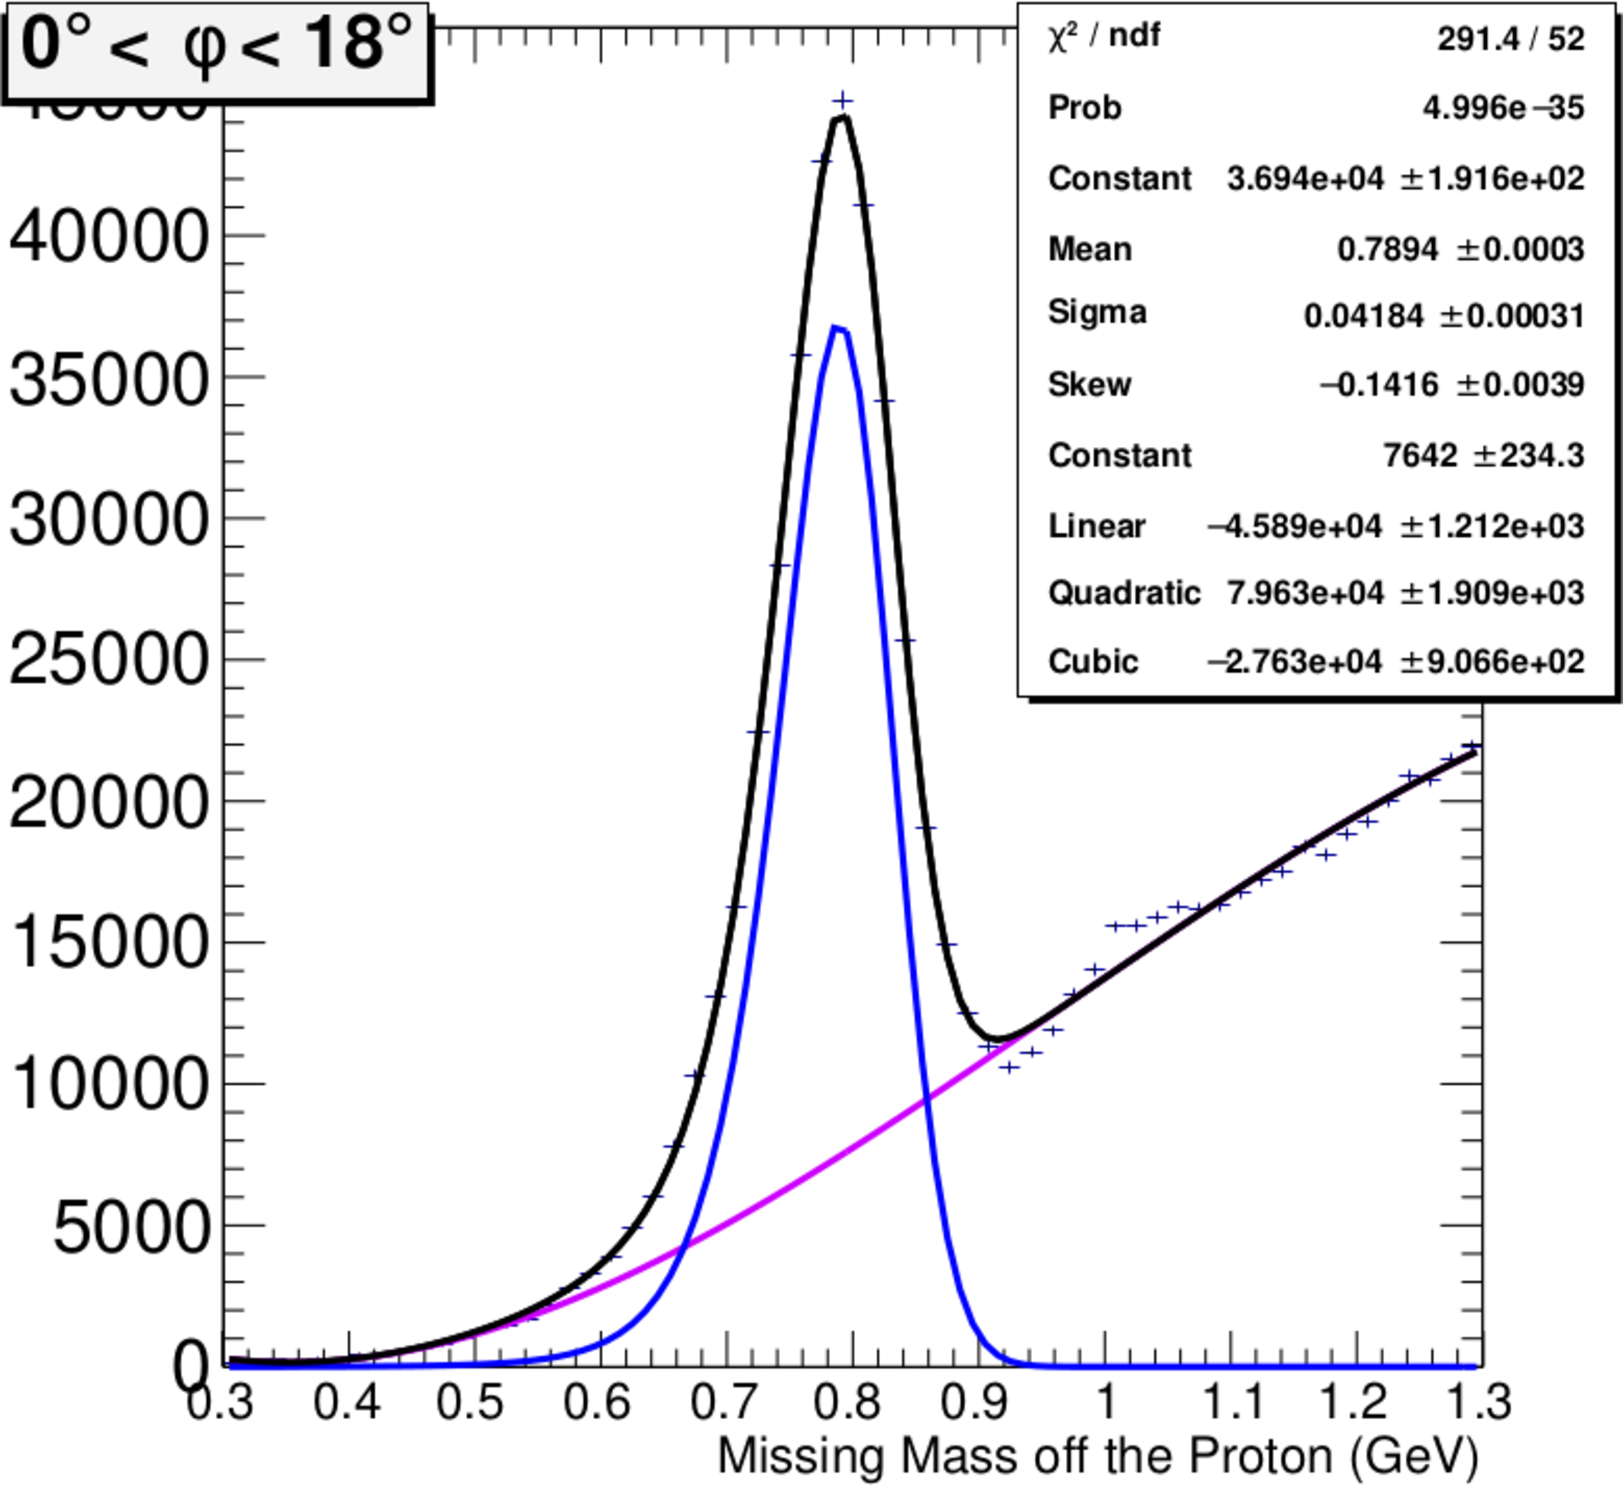
\includegraphics[width=0.45\textwidth]{figures/MissingOmegaFit.pdf}
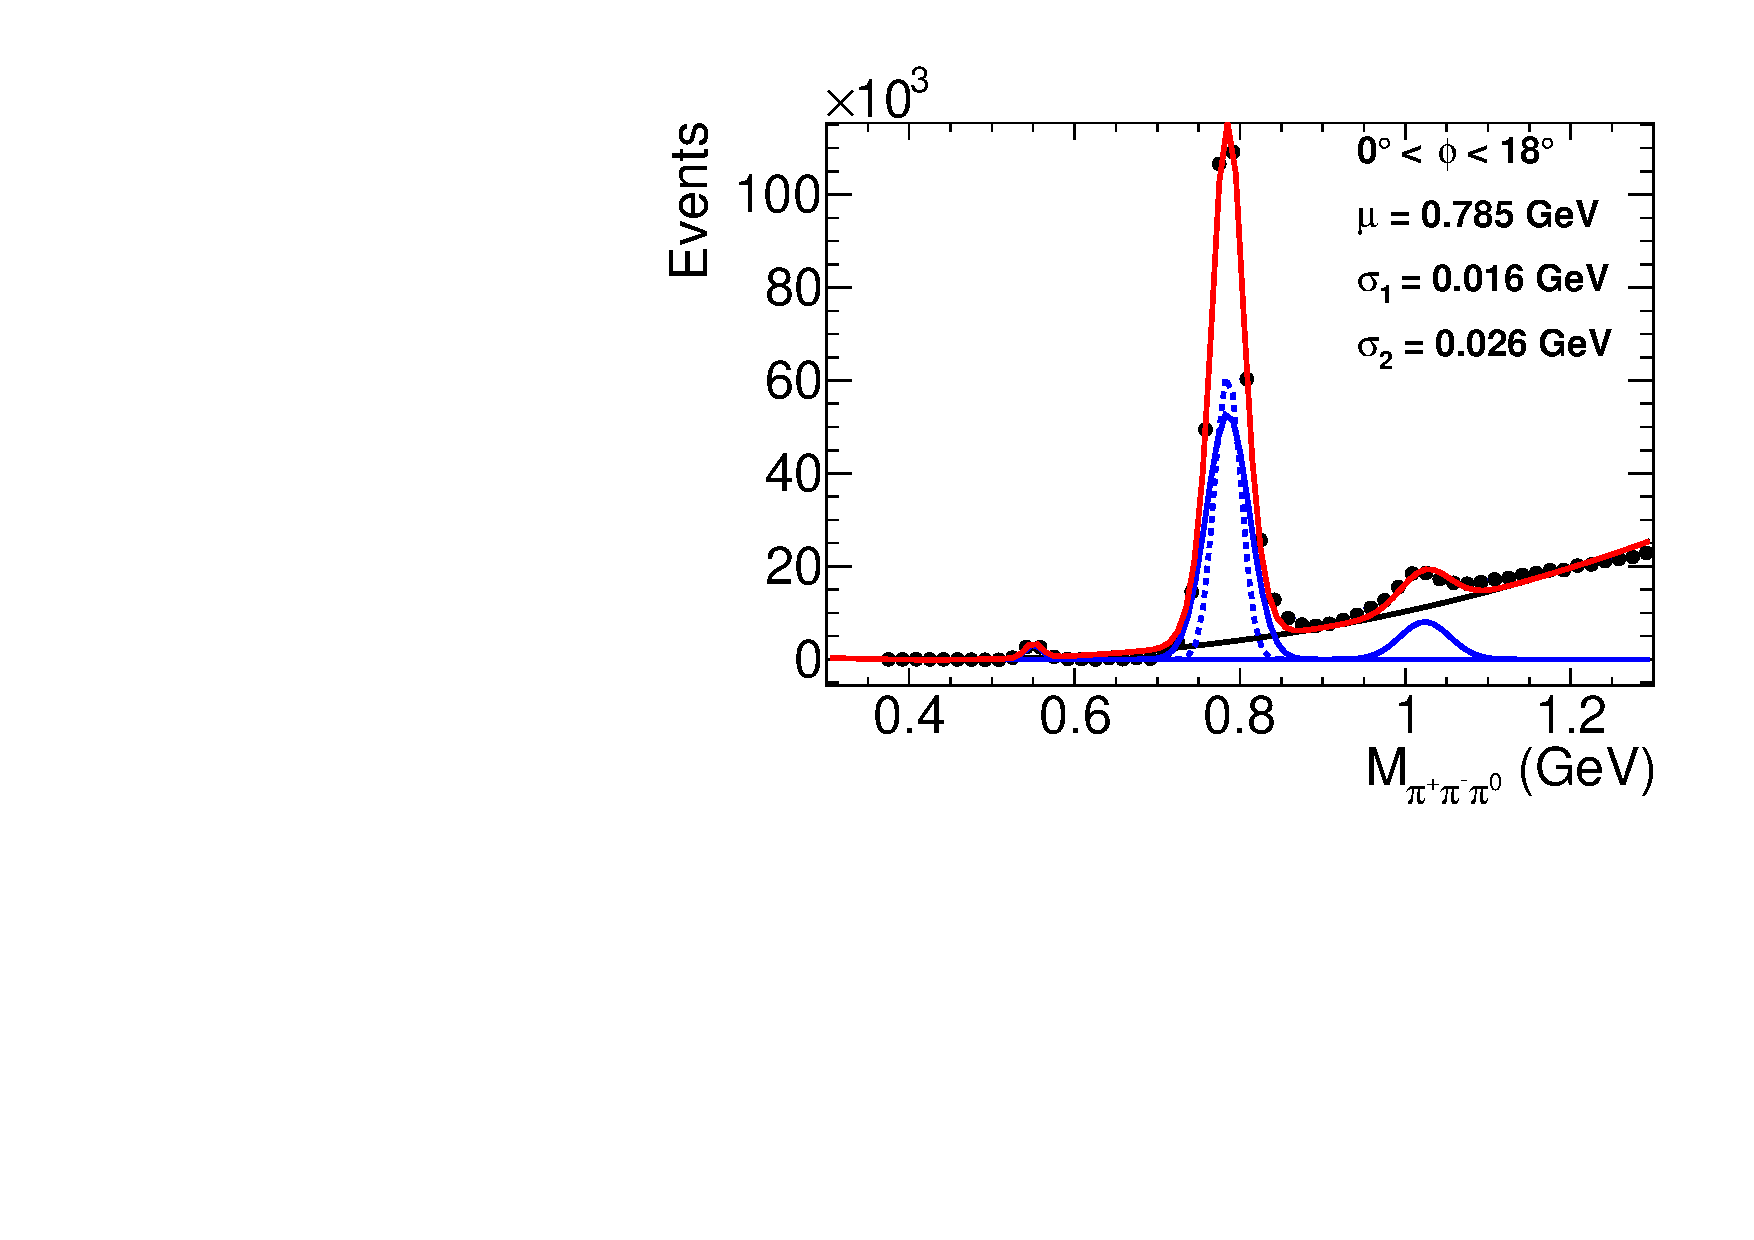
\includegraphics[width=0.45\textwidth]{figures/ThreePiFit.pdf}
\caption{\label{fig:omega mass}
Reconstructed mass distributions for the reaction $\gamma p \to p\pi^0\pi^{\pm}(\pi^\mp)$ for a bin in $\phi$.
  (Left) Distribution of the missing mass off the proton.
(Right) Invariant mass distribution for the $\pi^+\pi^-\pi^0$ system.  The black
curves show the results of fits to the distributions.
 (Color online)}
\end{center}
\end{figure}

\begin{figure}[tpb]
\begin{center}
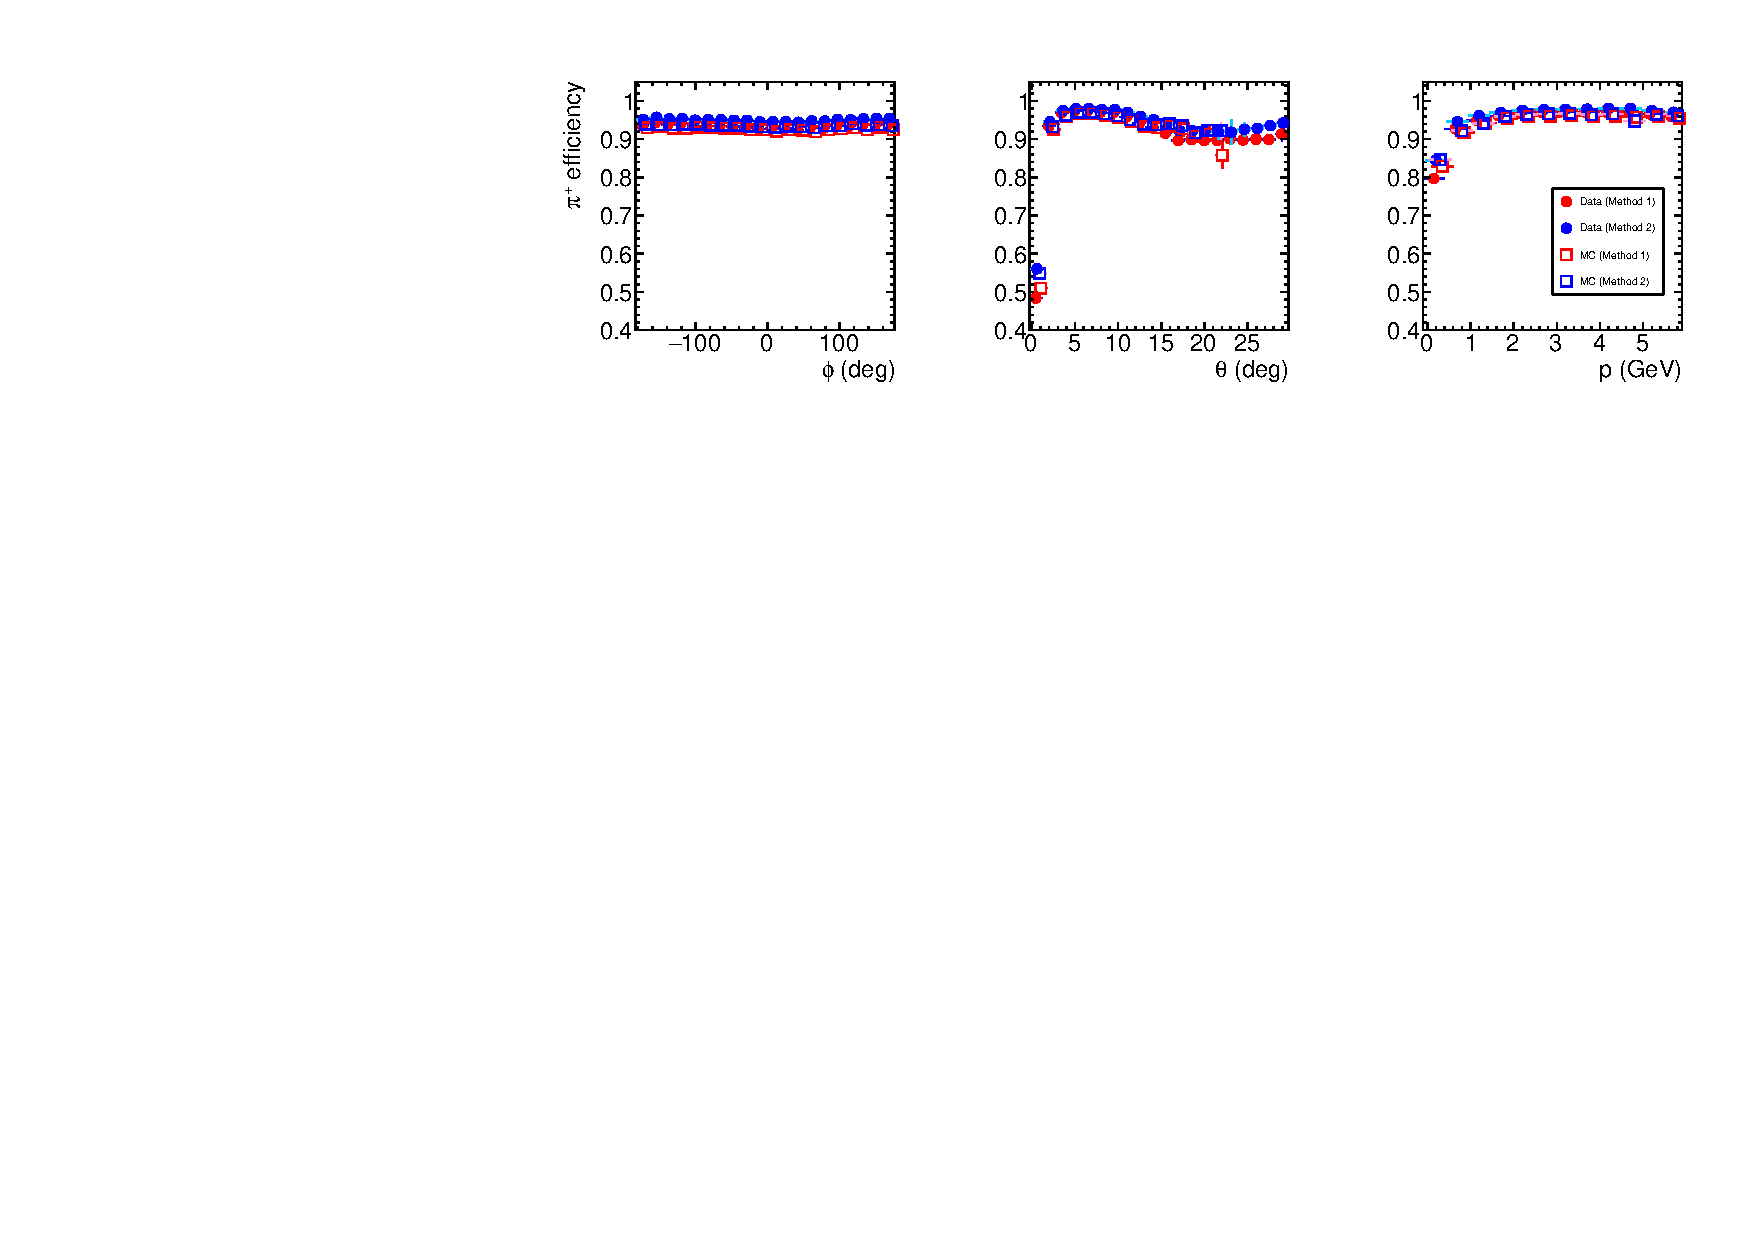
\includegraphics[width=\textwidth]{figures/PiPlusEfficiency.pdf}
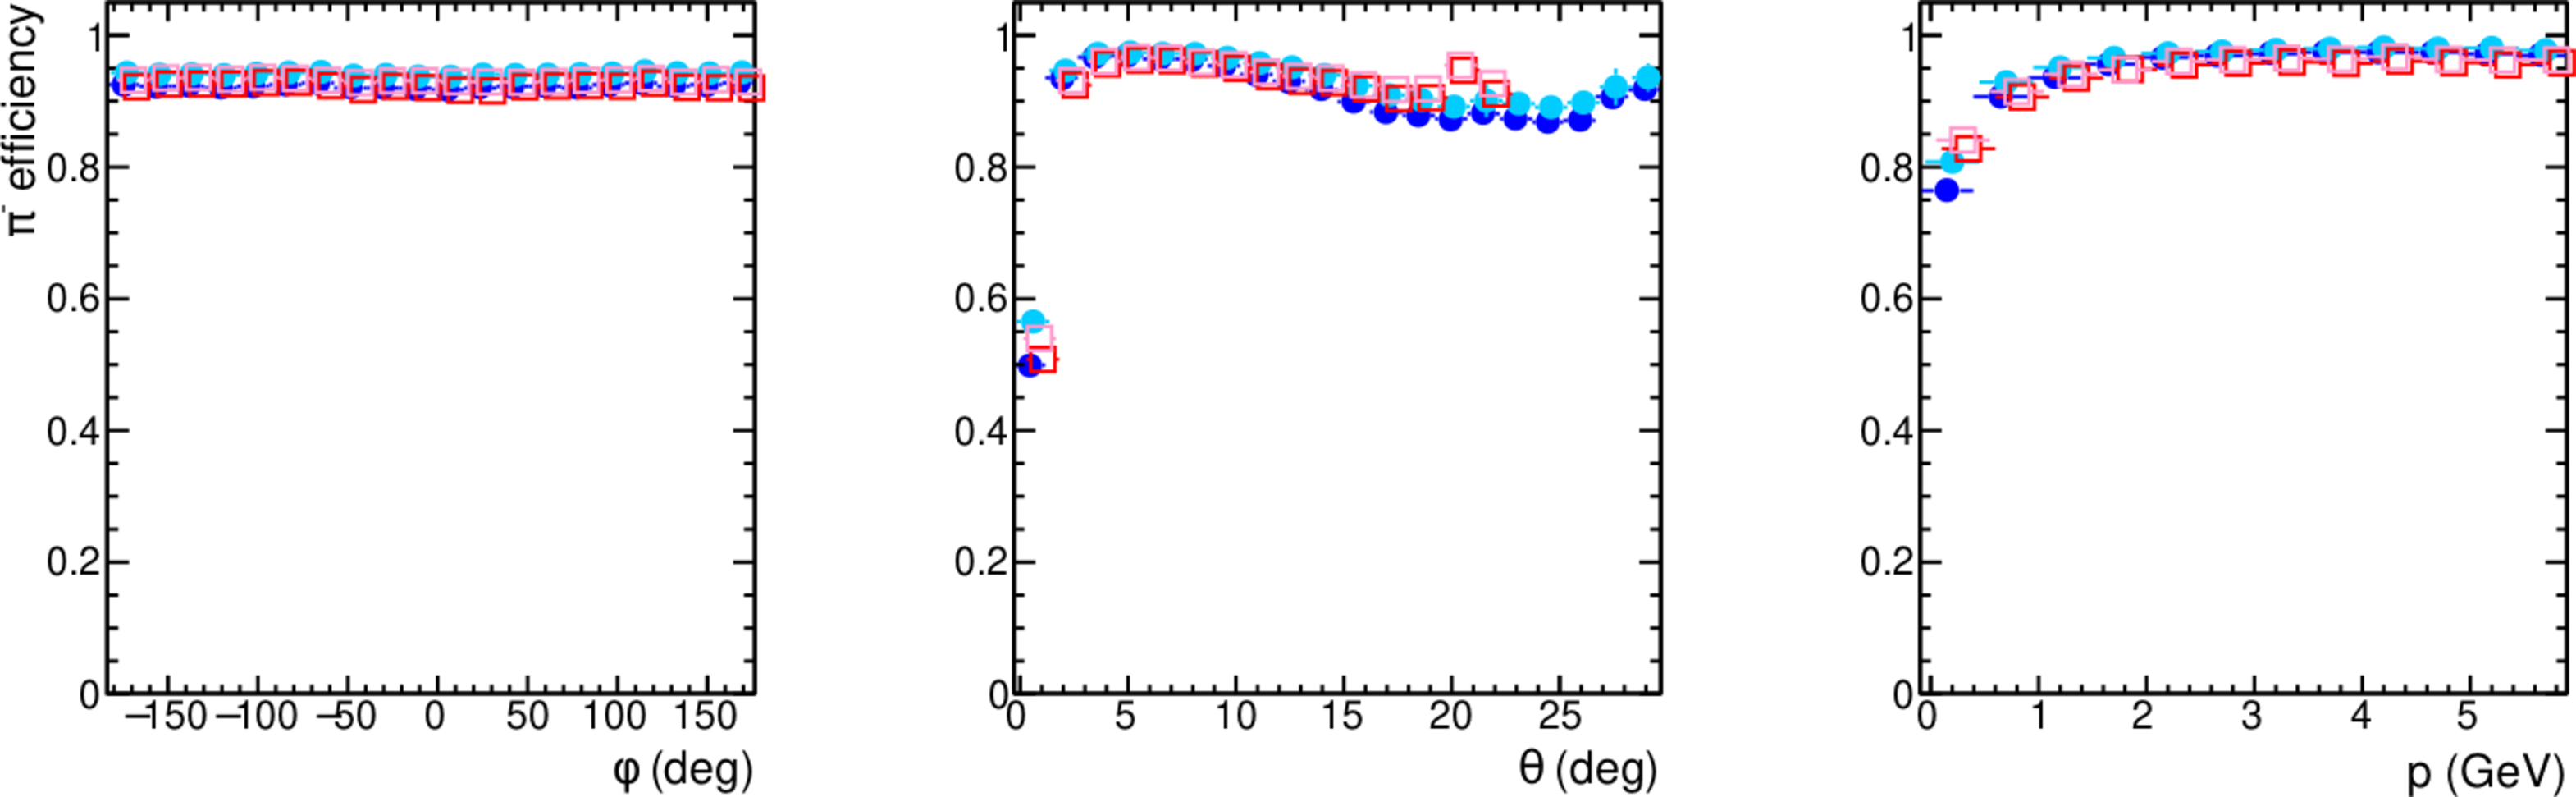
\includegraphics[width=\textwidth]{figures/PiMinusEfficiency.pdf}
\caption{\label{fig:tracking efficiency}
(Top row) Tracking efficiency for $\pi^+$ tracks. (Bottom row) Tracking efficiency for $\pi^-$ tracks.  (Color online)}
\end{center}
\end{figure}



\subsection{Photon efficiency\label{sec:perfneutral}}

%\subsubsection{Resolution \label{sec:perfneutralresol}}

%The invariant mass resolution of the decay $\eta \to \gamma \gamma$ has been found to primarily depend on the energy resolution of the calorimeters at \gx{}.  Therefore, in Fig.~X we show the resolution for these reconstructed decays for three classes of events: where both photons from the  $\eta \to \gamma \gamma$ are reconstructed in the BCAL, were both are reconstructed in the FCAL, and where one photon is reconstructed in the BCAL and one in the FCAL.

%\subsubsection{Efficiency \label{sec:perfneutraleff}}

Photon-reconstruction efficiency has been studied using different methods for the FCAL and BCAL.  In the FCAL, absolute photon reconstruction efficiencies have been determined using the ``tag-and-probe'' method with a sample of photons from the reaction $\gamma p \to \omega p$, $\omega \to \pi^+\pi^-\pi^0$, $\pi^0 \to \gamma (\gamma)$, where one final photon is allowed but not required to be reconstructed.  The yields with and without the reconstructed photon are determined using two methods.  In the first method, the $\omega$ yield is determined from the missing-mass spectrum, $M_X(\gamma p \rightarrow pX)$, selecting on whether only one or both reconstructed photons are consistent with a final-state $\pi^0$. In the second method,  the count when both photons are found is determined from the $\omega$ yield from the fully reconstructed invariant mass $M(\pi^+\pi^-\gamma\gamma)$. If the photon is not reconstructed, the $\omega$ yield is determined by a fit to the distribution of the missing mass off the proton.  Both methods yield consistent results, with a reconstruction efficiency generally above 90\%, and within 5\% or less agree with the efficiencies determined from simulation.

\begin{figure}[tbp]
\begin{center}
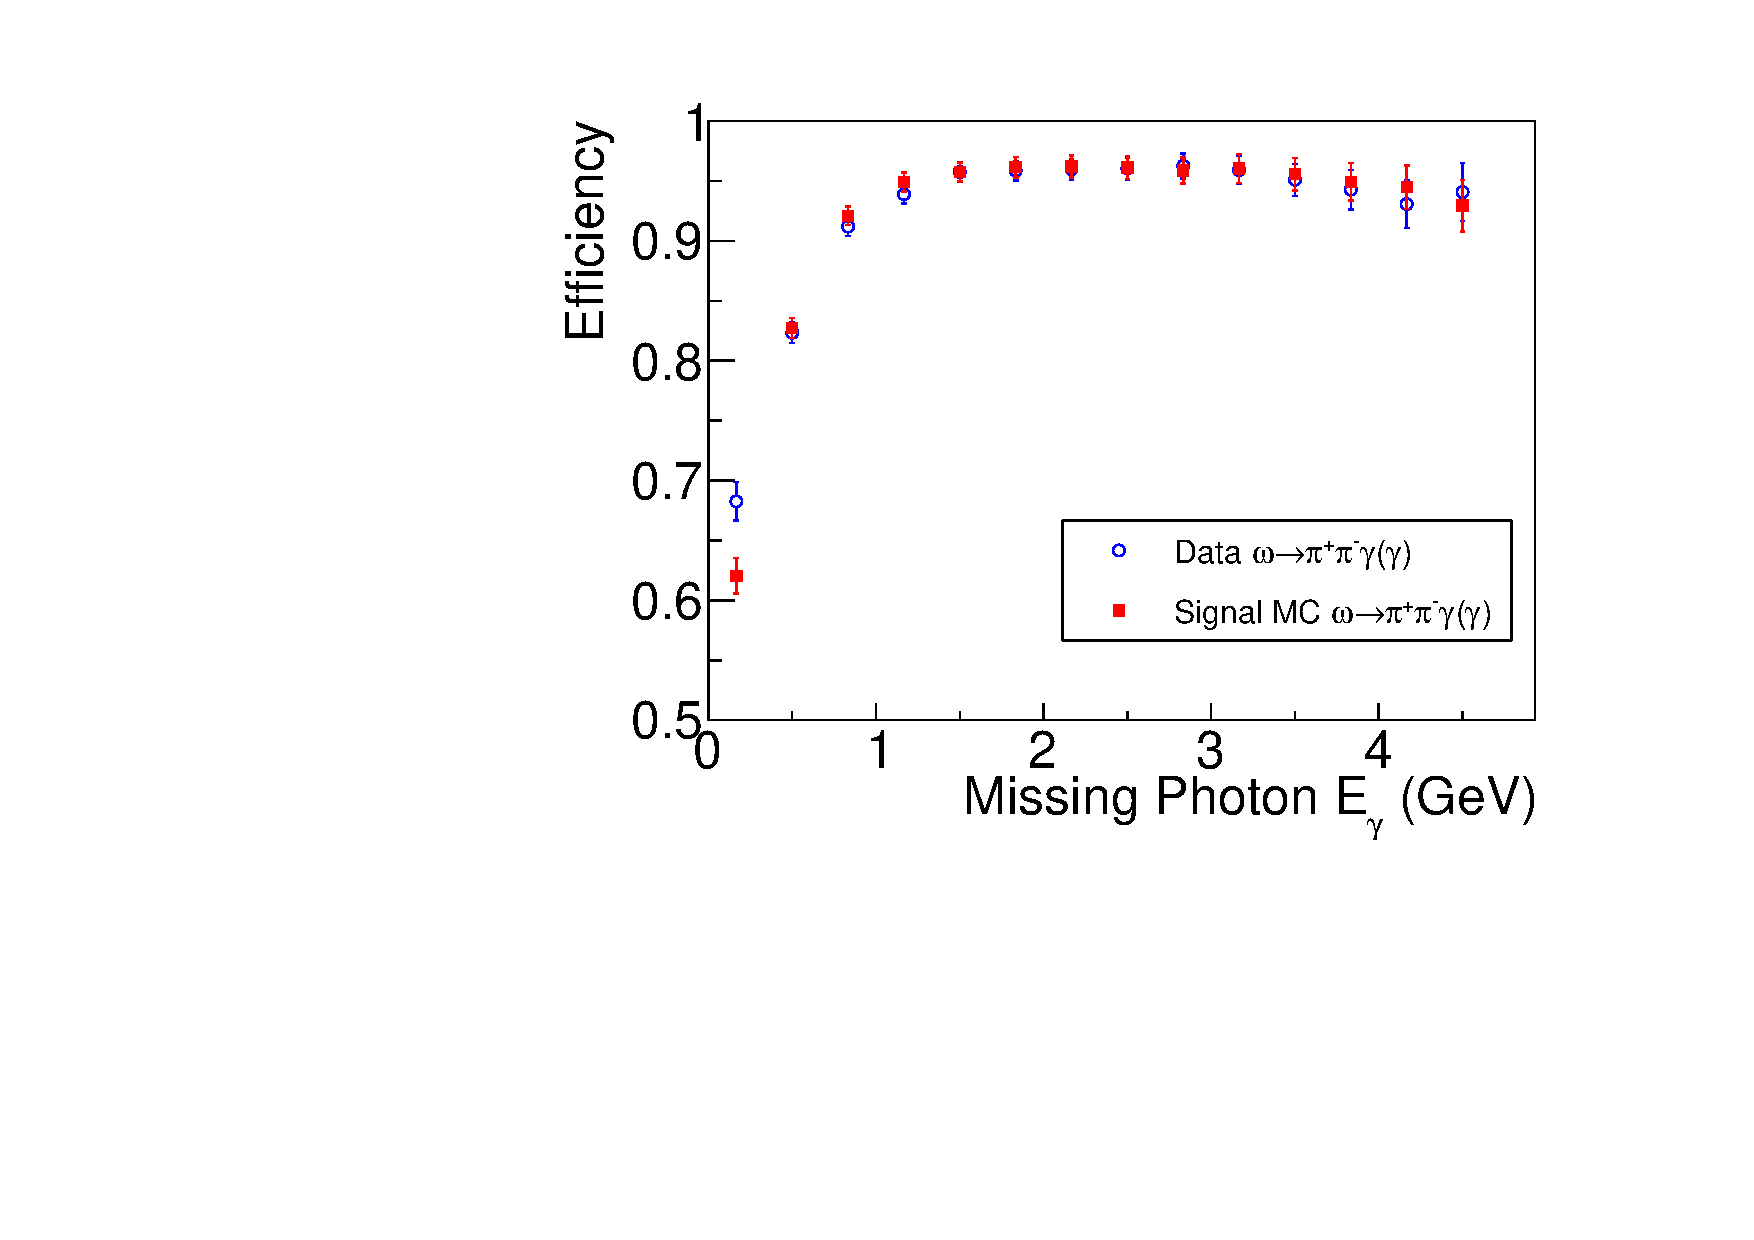
\includegraphics[width=0.45\textwidth]{figures/OmegaCompareE.pdf}
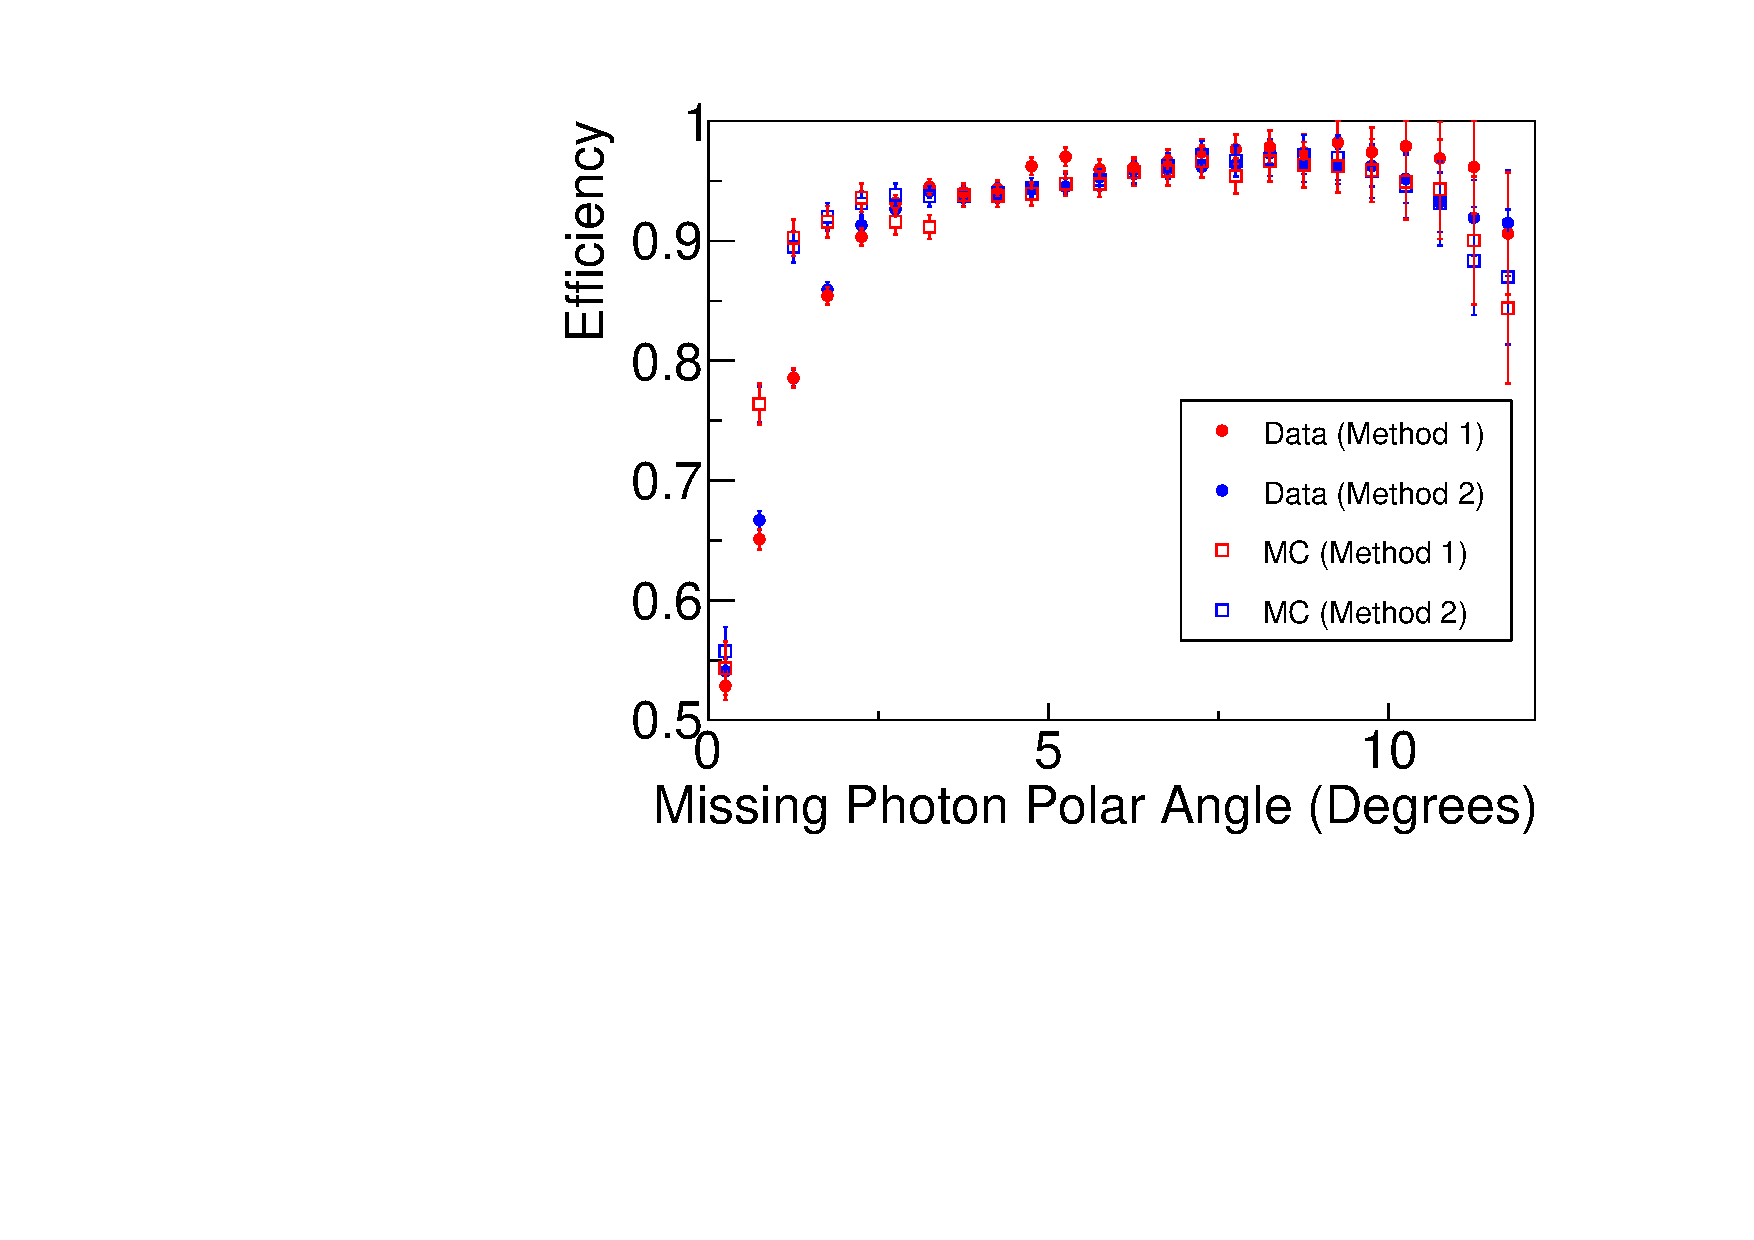
\includegraphics[width=0.45\textwidth]{figures/OmegaCompareTheta.pdf}
\caption{\label{fig:fcalphotoneff}
Photon reconstruction efficiency in FCAL determined from $\gamma p \to \omega p$, $\omega \to \pi^+\pi^-\pi^0$, $\pi^0 \to \gamma (\gamma)$ as a function of (left) photon energy and (right) photon polar angle.  Good agreement between data and simulation is observed in the fiducial region $\theta = 2^\circ - 10.6^\circ$. (Color online)
}
\end{center}
\end{figure}

A relative photon efficiency determination has been performed using $\pi^0\to\gamma\gamma$ decays, which spans the full angular range detected in \gx{}.  A sample of fully reconstructed $\gamma p \to  \pi^+\pi^-\pi^0 p$ events were inspected, taking advantage of the $\pi^0\to\gamma\gamma$ decay isotropy in the center-of-mass frame.  Thus, any anisotropy indicates an inefficiency in the detector. Results from this analysis are illustrated in Fig.~\ref{fig:bcalpi0photoneff}. Generally, this relative efficiency is above 90\%, and agrees within 5\% of that determined from simulation.  

The models for the simulated response of both calorimeters are being updated, and the final agreement between photon efficiency determined in data and simulation is expected to improve.

\begin{figure}[tbp]
\begin{center}
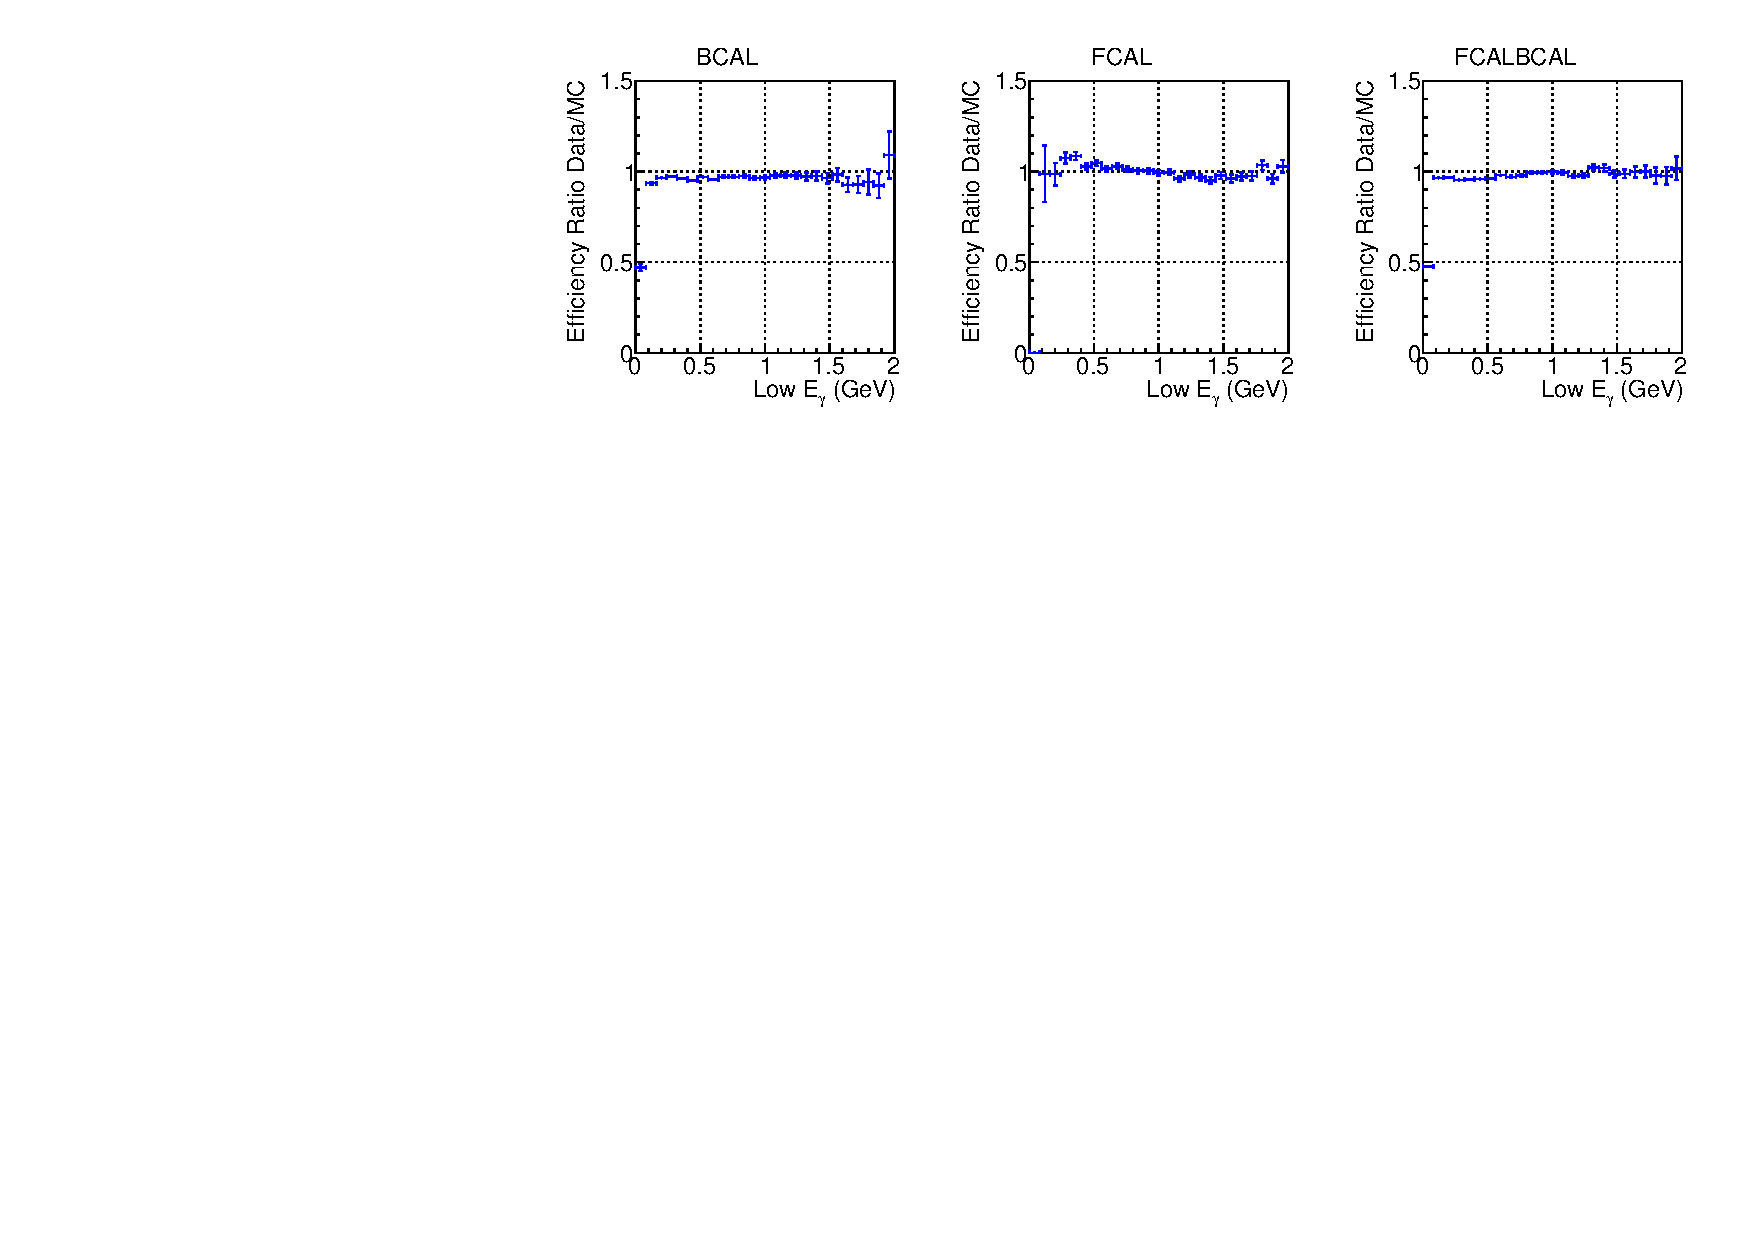
\includegraphics[width=\textwidth]{figures/plot_CostheEff_NIM_jun19.pdf}
\caption{\label{fig:bcalpi0photoneff}
Ratios of relative photon reconstruction efficiency between data and simulation determined from $\pi^0\to\gamma \gamma$ decays in $\gamma p \to  \pi^+\pi^-\pi^0 p$ events.  The efficiency ratios are shown for the cases where (left) both photons were measured in the BCAL, (middle) both photons were measured in the FCAL, and (right) one photon was measured in the BCAL and the other in the FCAL.
}
\end{center}
\end{figure}


Detailed studies of detector performance determined the standard fiducial region for most analyses to be $\theta = 2^\circ - 10.6^\circ$ and $\theta > 11.3^\circ$.  These requirements avoid the region dominated by beam-related backgrounds at small $\theta$ and the transition region between the BCAL and FCAL, where shower reconstruction is difficult.

\subsection{Kinematic fitting \label{sec:perffitting}}

Kinematic fitting is a powerful tool to improve the resolution of measured data and to distinguish between different reactions.  In \gx{}, this method takes advantage of the fact that the initial state is very well known, with the target proton at rest, and the incident photon energy measured with very high precision ($<0.1\%$). This knowledge of the initial state gives substantial improvements in the kinematic quantities determined for exclusive reactions.  The most common kinematic fits that are performed are those that impose energy-momentum conservation between the initial and final-state particles.  Additional optional constraints in these fits are for the four-momenta of the daughters of an intermediate particle to add up to a fixed invariant mass, and for all the particles to come from a common vertex (or multiple vertices, in the case of reactions containing long-lived, decaying particles).

To illustrate the performance of the kinematic fit, we use a sample of $\gamma p \to \eta p$, $\eta \to \pi^+\pi^-\pi^0$ events selected using a combination of standard particle identification and simple kinematic selections.  
%Fig.~\ref{fig:etakinfit} shows the $\eta\to \pi^+\pi^-\pi^0$ peak and the improvement in $\pi^+\pi^-\pi^0$ mass resolution using the kinematic fit from 2.6~MeV to 1.7~MeV, which is typical of low-multiplicity meson production reactions.  
The use of the kinematic fit improves the $\eta$-mass resolution  from  2.6~MeV to 1.7~MeV, which is typical of low-multiplicity meson production reactions.  
The quality of the kinematic fit is determined using either the probability calculated from the $\chi^2$ of the fit and the number of degrees-of-freedom or the $\chi^2$ of the fit itself. 
The distributions of the kinematic fit $\chi^2$ and probability are illustrated in Fig.~\ref{fig:kinfitperform} for both reconstructed and simulated data.  The agreement between the two distributions is good for small $\chi^2$ (large probability), and flat over most of the probability range, indicating good overall performance for most signal events.  The disagreement between the two distributions at larger $\chi^2$ (probability $<0.2$) is due to a combination of background events and deficiencies in the modelling of poorly measured events with large resolution.

The performance of the reconstruction algorithms and kinematic fit can be studied through investigating the ``pull'' distributions, where the pull of a variable $x$ is defined by comparing its measured values and uncertainties and those resulting from the kinematic fit as
\begin{equation}
    \text{pull}_x = \frac{x_\text{fitted} - x_\text{measured}}{\sqrt{\sigma_{x,\text{measured}}^2 - \sigma_{x,\text{fitted}}^2}}.
\end{equation}
If the parameters and covariances of reconstructed particles are Gaussian, are measured accurately, and the fit is performing correctly, then these pull values are expected to have a Gaussian distribution centered at zero with a width $\sigma$ of 1.  If the pull distributions are not centered at zero, this is an indication that there is a bias in the measurements or the fit.  If $\sigma$ varies from unity, this is an indication that the covariance matrix elements are not correctly estimated.  

As an example, the pull distributions for the momentum components of the $\pi^-$ in reconstructed $\gamma p \to \eta p$, $\eta \to \pi^+\pi^-\pi^0$ events are shown in Fig.~\ref{fig:kinfitpulls}.  Both real and simulated data have roughly Gaussian shapes with similar widths.  More insight into the stability of the results of the kinematic fit can be found by studying the variation of the means and widths of the fit distributions as a function of the fit probability.  The results of such a study are summarized in Fig.~\ref{fig:kinfitstudy}, where broad agreement between the results from real and simulated data is seen.  The means of the pull distributions are generally around zero (with $p_x$ and its mean of roughly $-0.1$ a notable exception), and the widths within about 20\% of unity.  This level of performance and agreement between data and simulation is acceptable for the initial analysis of data, where very loose cuts on the kinematic fit $\chi^2$ are performed, and steady improvement in the modeling of the covariance matrices of reconstructed particles is expected to continue.


\begin{figure}[tbp]
\begin{center}
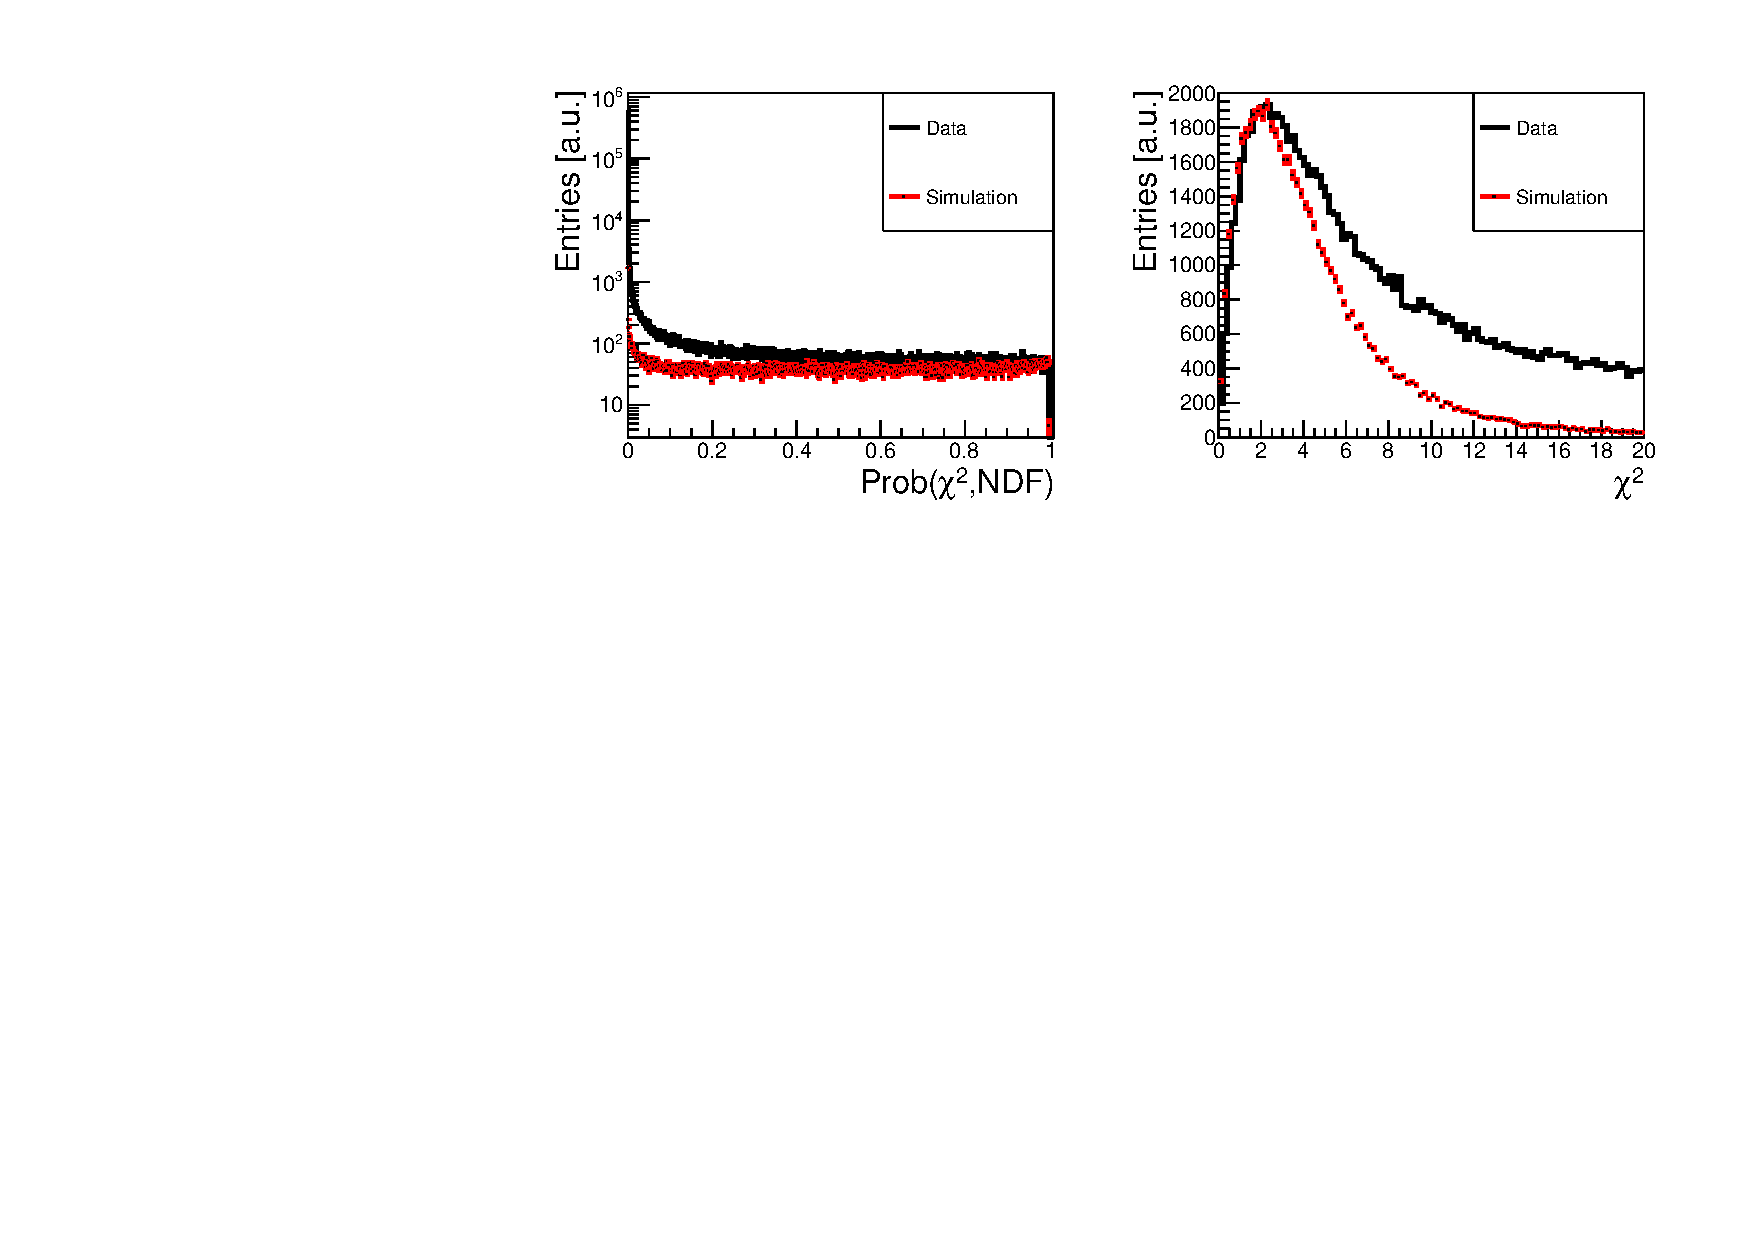
\includegraphics[width=0.75\textwidth]{figures/gluex_nim_kfit_prob.pdf}
\caption{\label{fig:kinfitperform}
Distribution of kinematic fit (left) probability and (right) $\chi^2$ for reconstructed $\gamma p \to \eta p$,  $\eta \to \pi^+\pi^-\pi^0$ events in data and simulation.  Both distributions agree reasonably for well-measured events, and diverge due to additional background in data and differences in modeling poorly-measured events.
 (Color online)}
\end{center}
\end{figure}

\begin{figure}[tbp]
\begin{center}          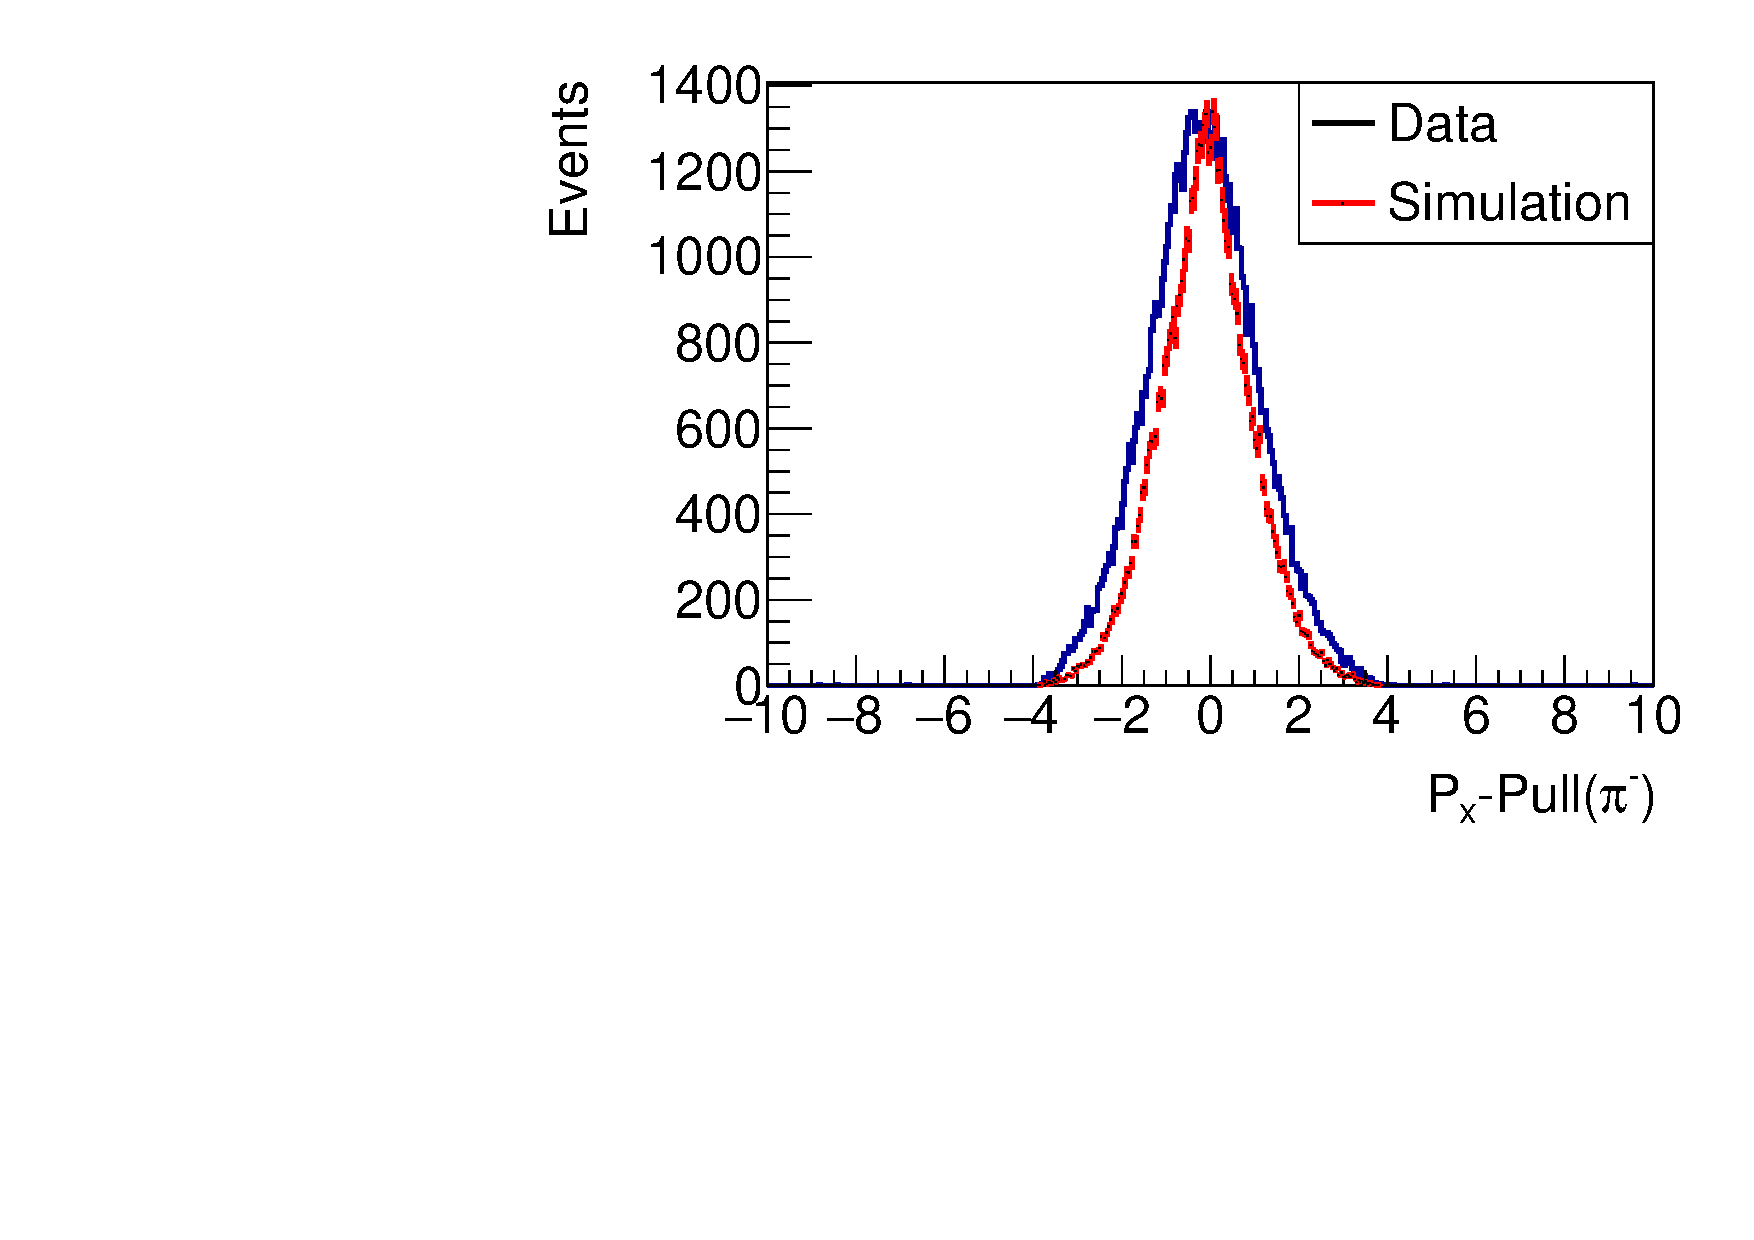
\includegraphics[width=0.29\textwidth]{figures/gluex_nim_PiMinus_PxPull.pdf}
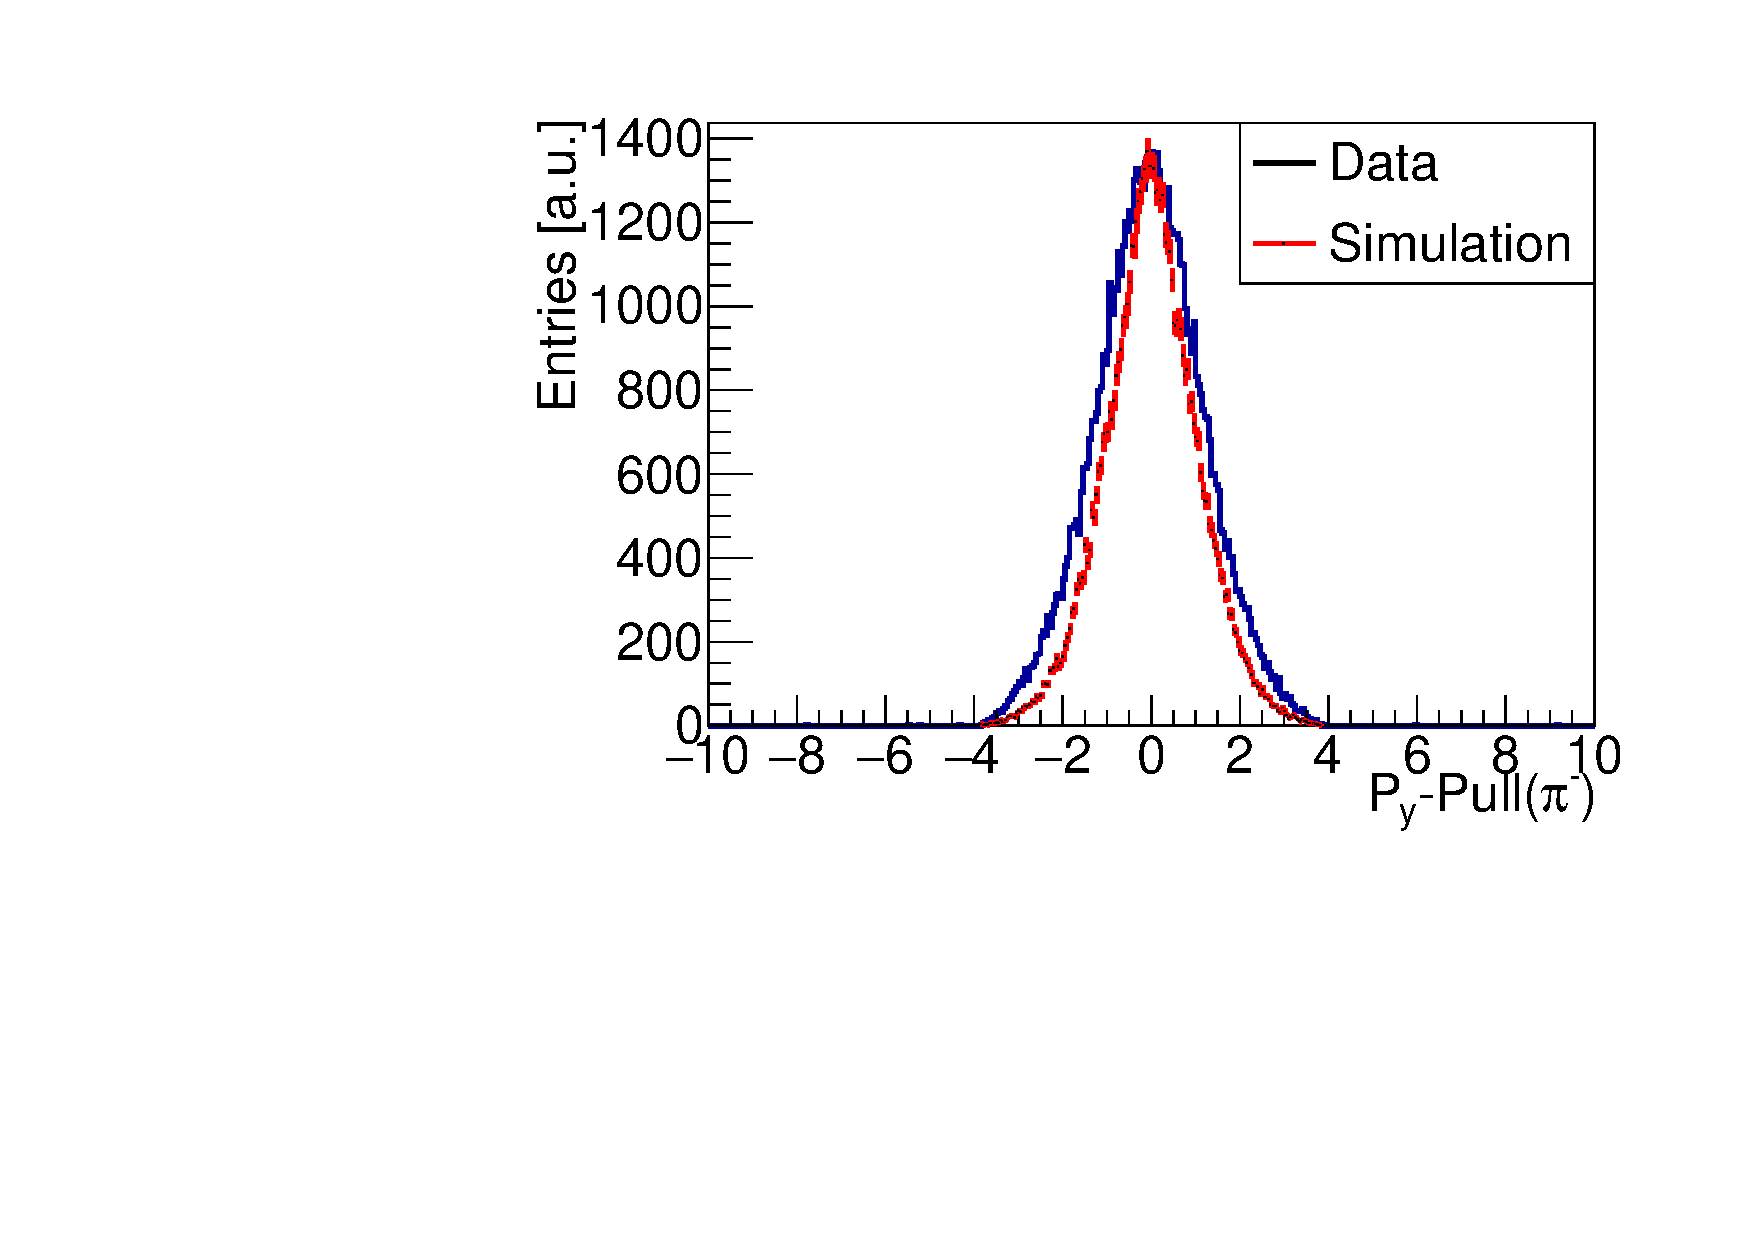
\includegraphics[width=0.29\textwidth]{figures/gluex_nim_PiMinus_PyPull.pdf}
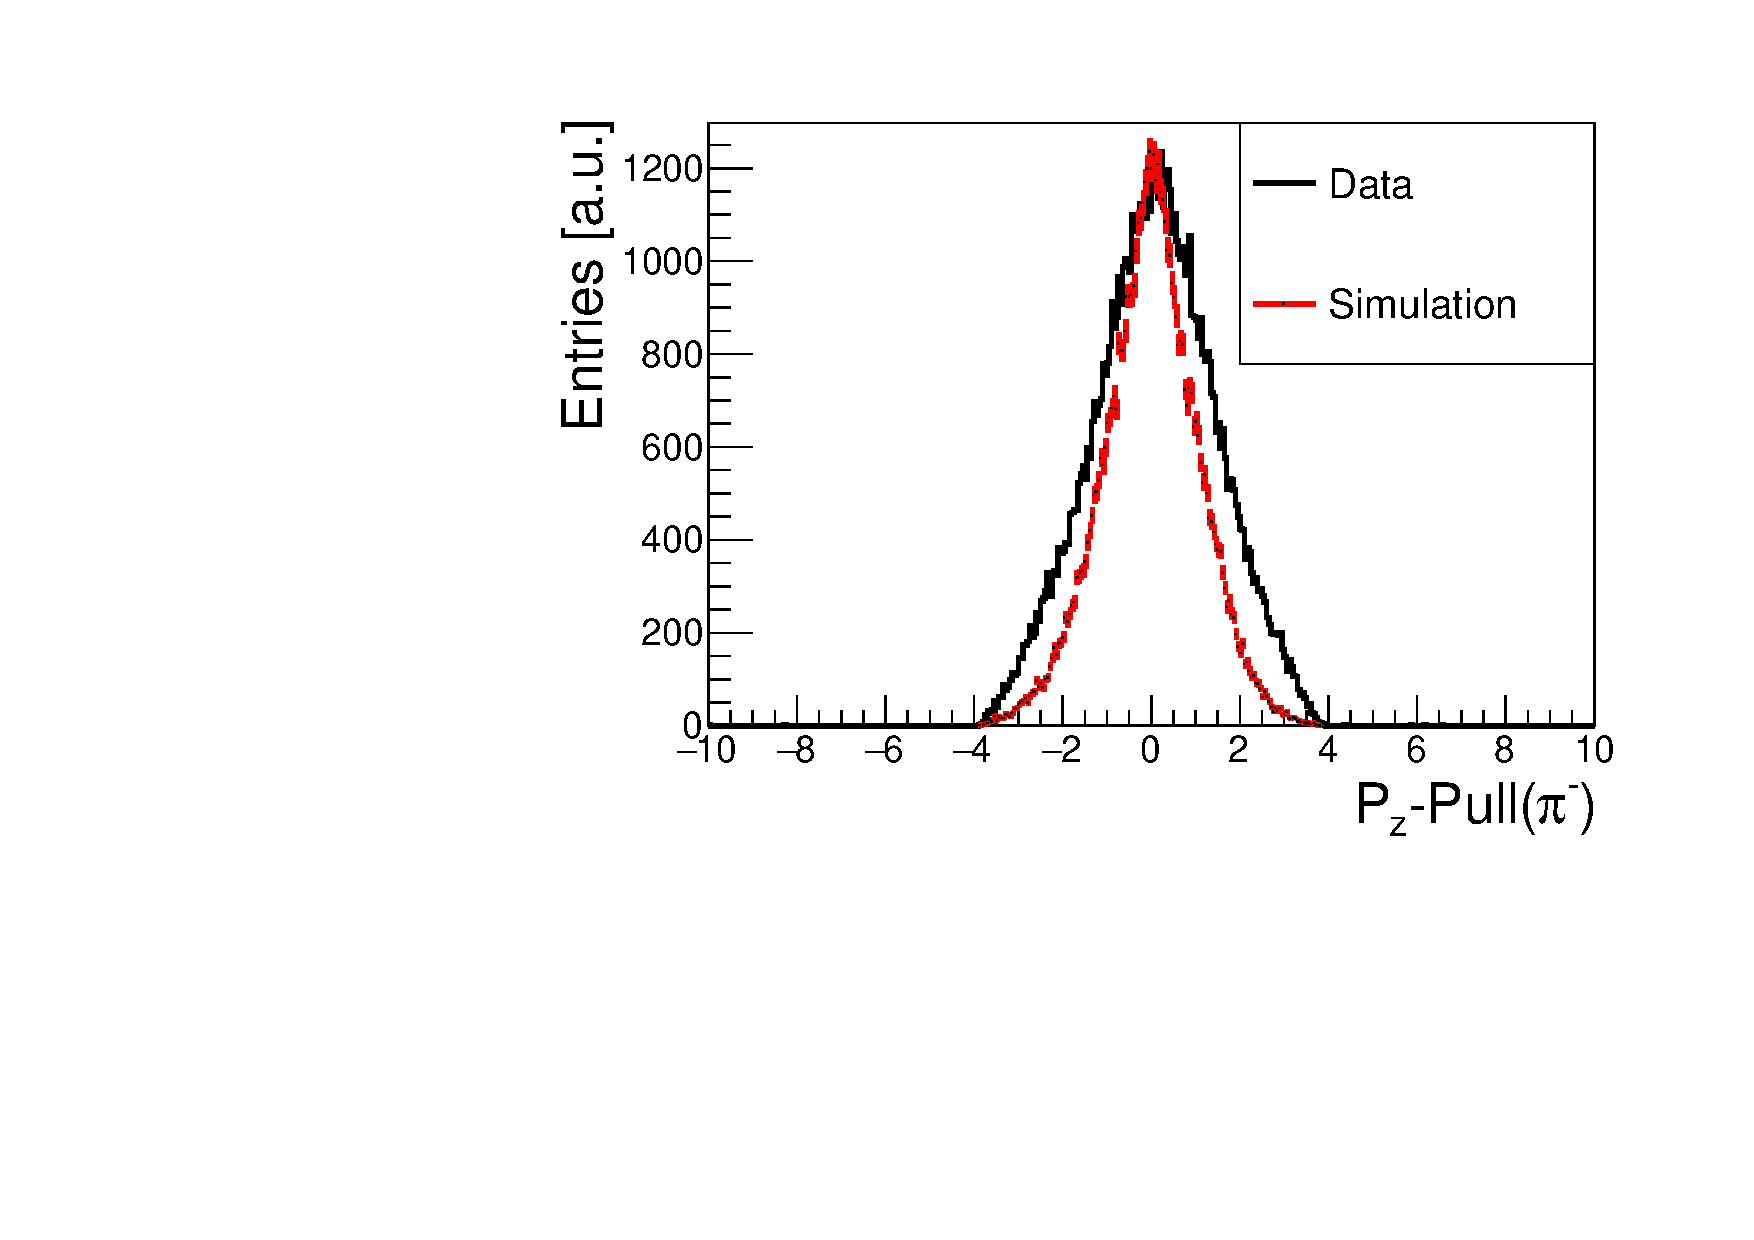
\includegraphics[width=0.29\textwidth]{figures/gluex_nim_PiMinus_PzPull.pdf}

\caption{\label{fig:kinfitpulls}
Pull distributions for momentum components of the $\pi^-$ from reconstructed $\gamma p \to \eta p$,  $\eta \to \pi^+\pi^-\pi^0$ events in data and simulation for events with fit probability $>0.01$: (left) $p_x$, (center) $p_y$, (right) $p_z$.
 (Color online)}
\end{center}
\end{figure}

\begin{figure}[tbp]
\begin{center}          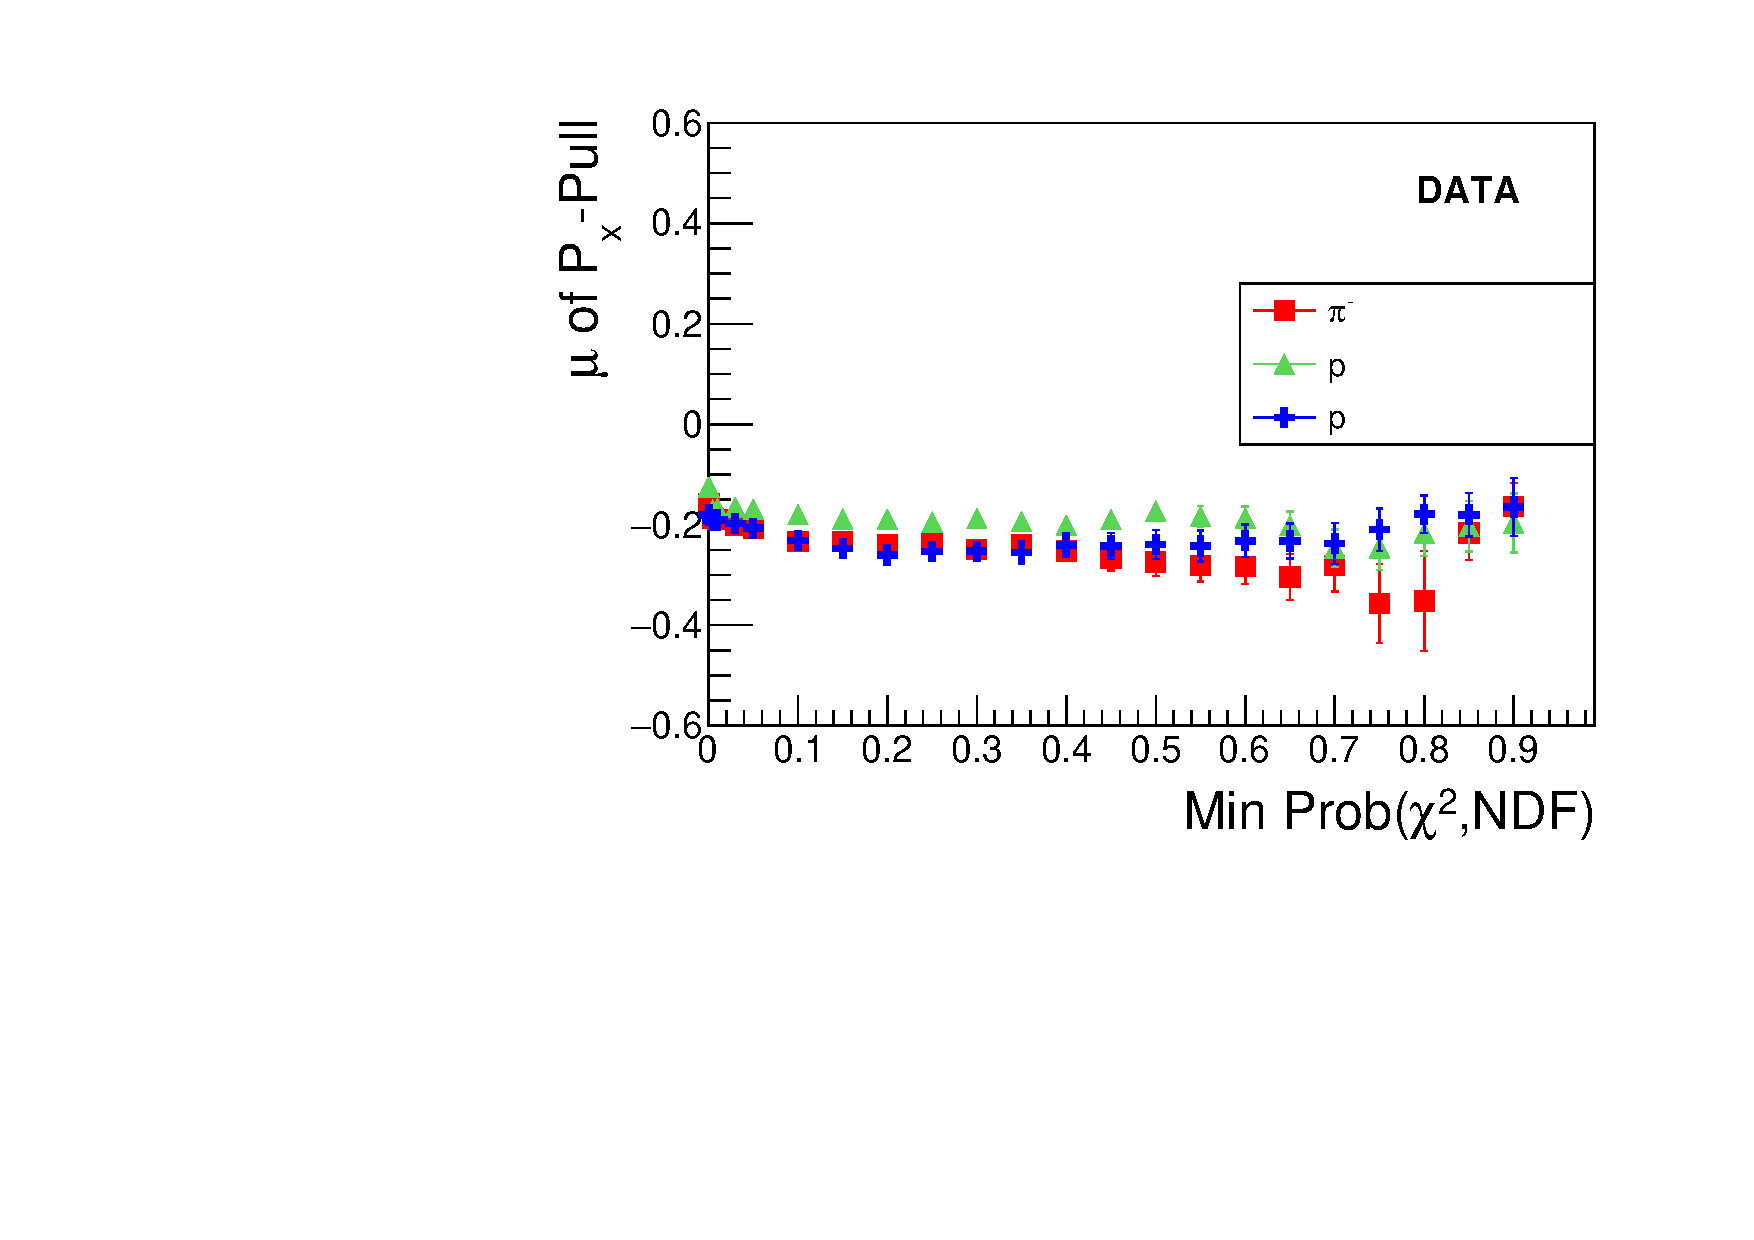
\includegraphics[width=0.3\textwidth]{figures/gluex_nim_pullspx_pulls_mean_data.pdf}
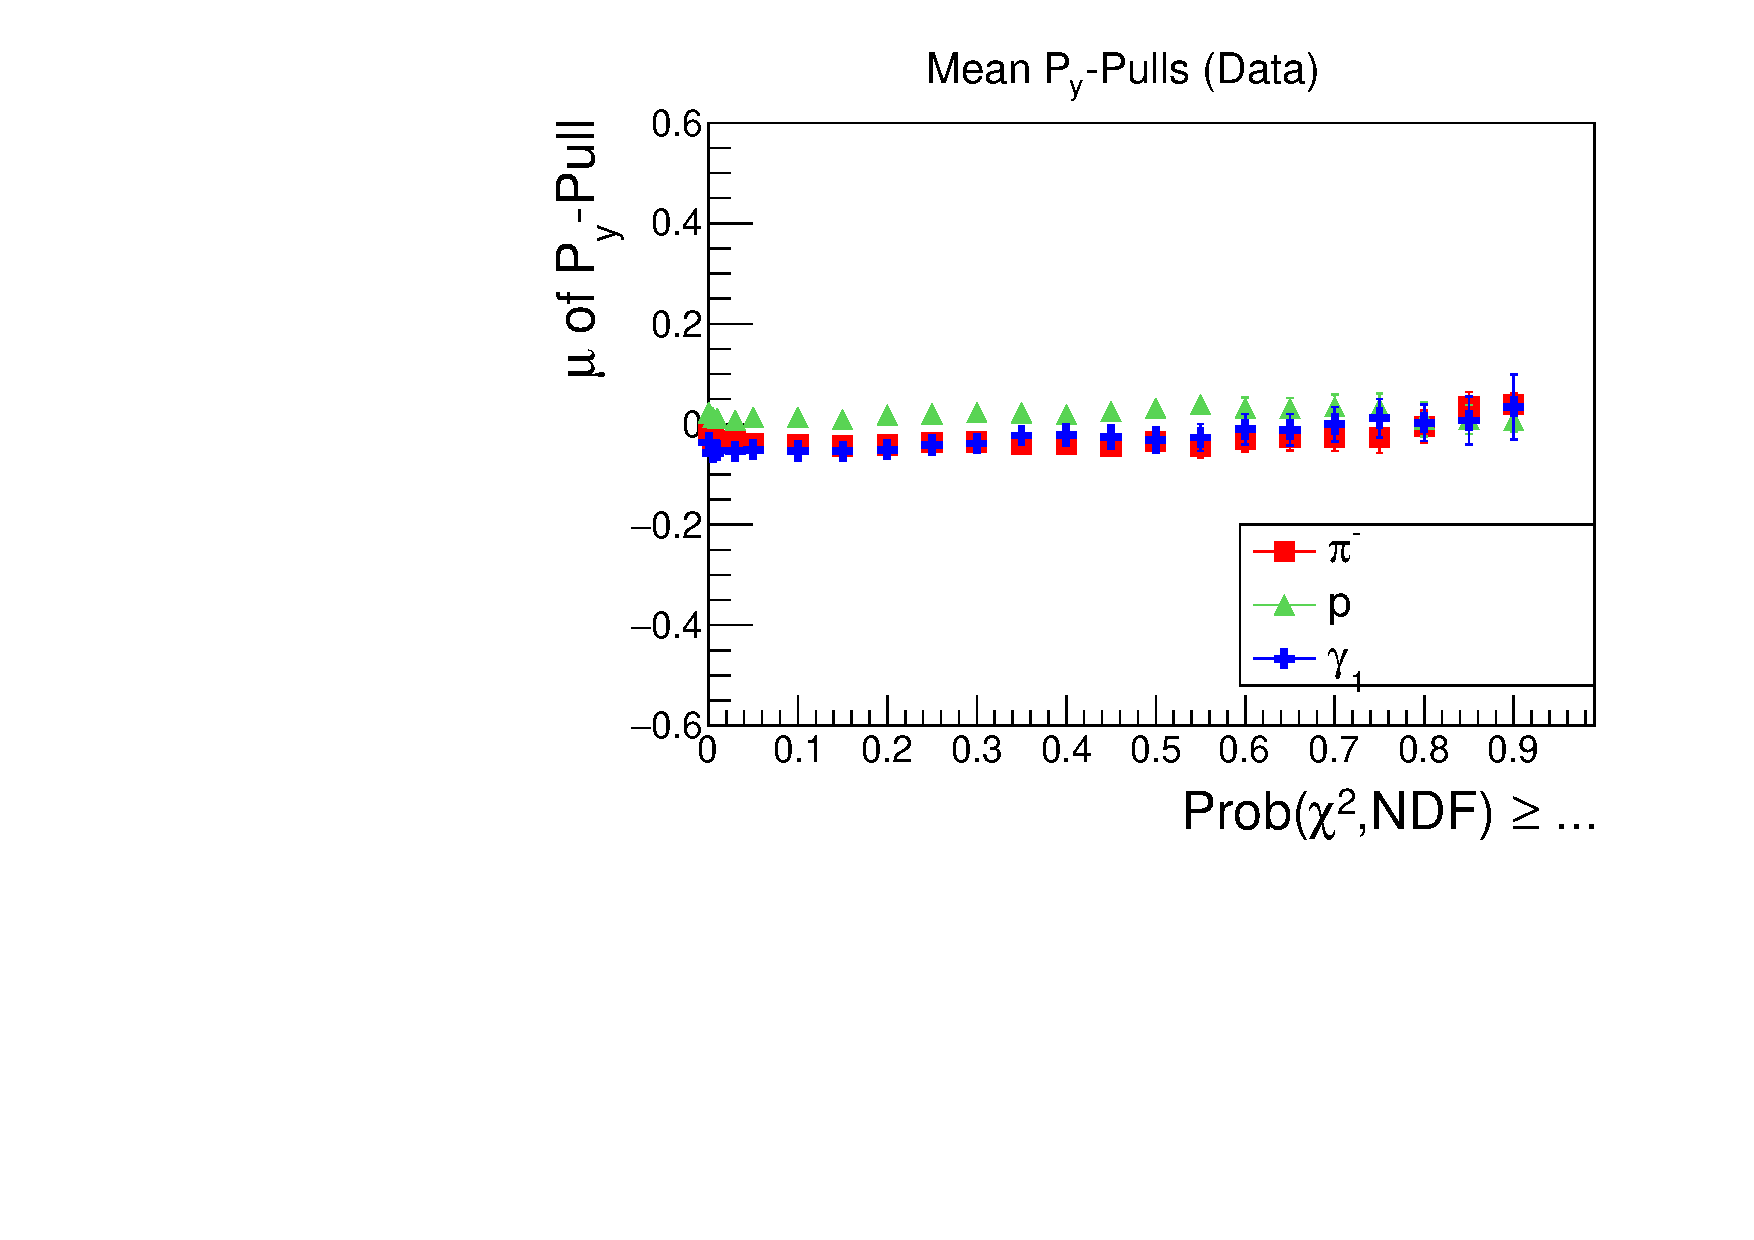
\includegraphics[width=0.3\textwidth]{figures/gluex_nim_pullspy_pulls_mean_data.pdf}
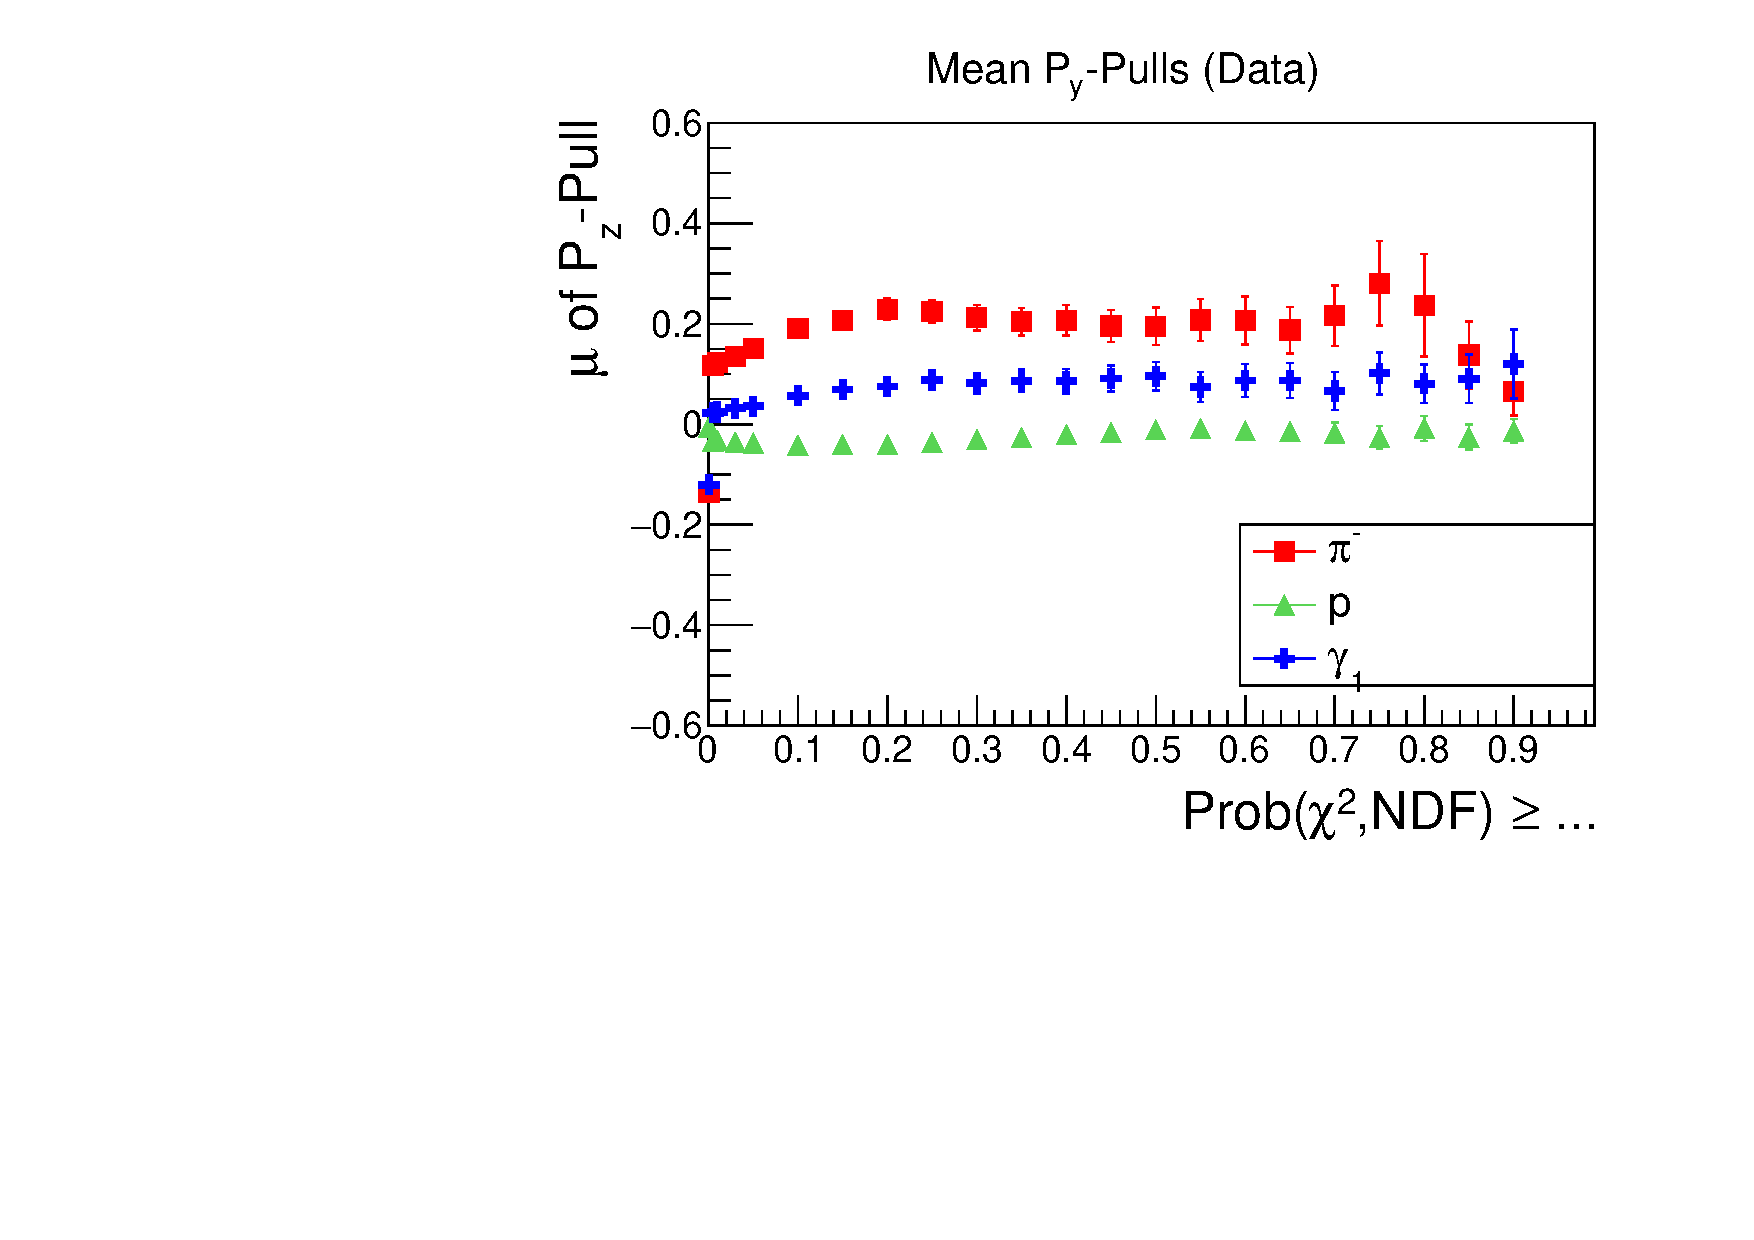
\includegraphics[width=0.3\textwidth]{figures/gluex_nim_pullspz_pulls_mean_data.pdf}

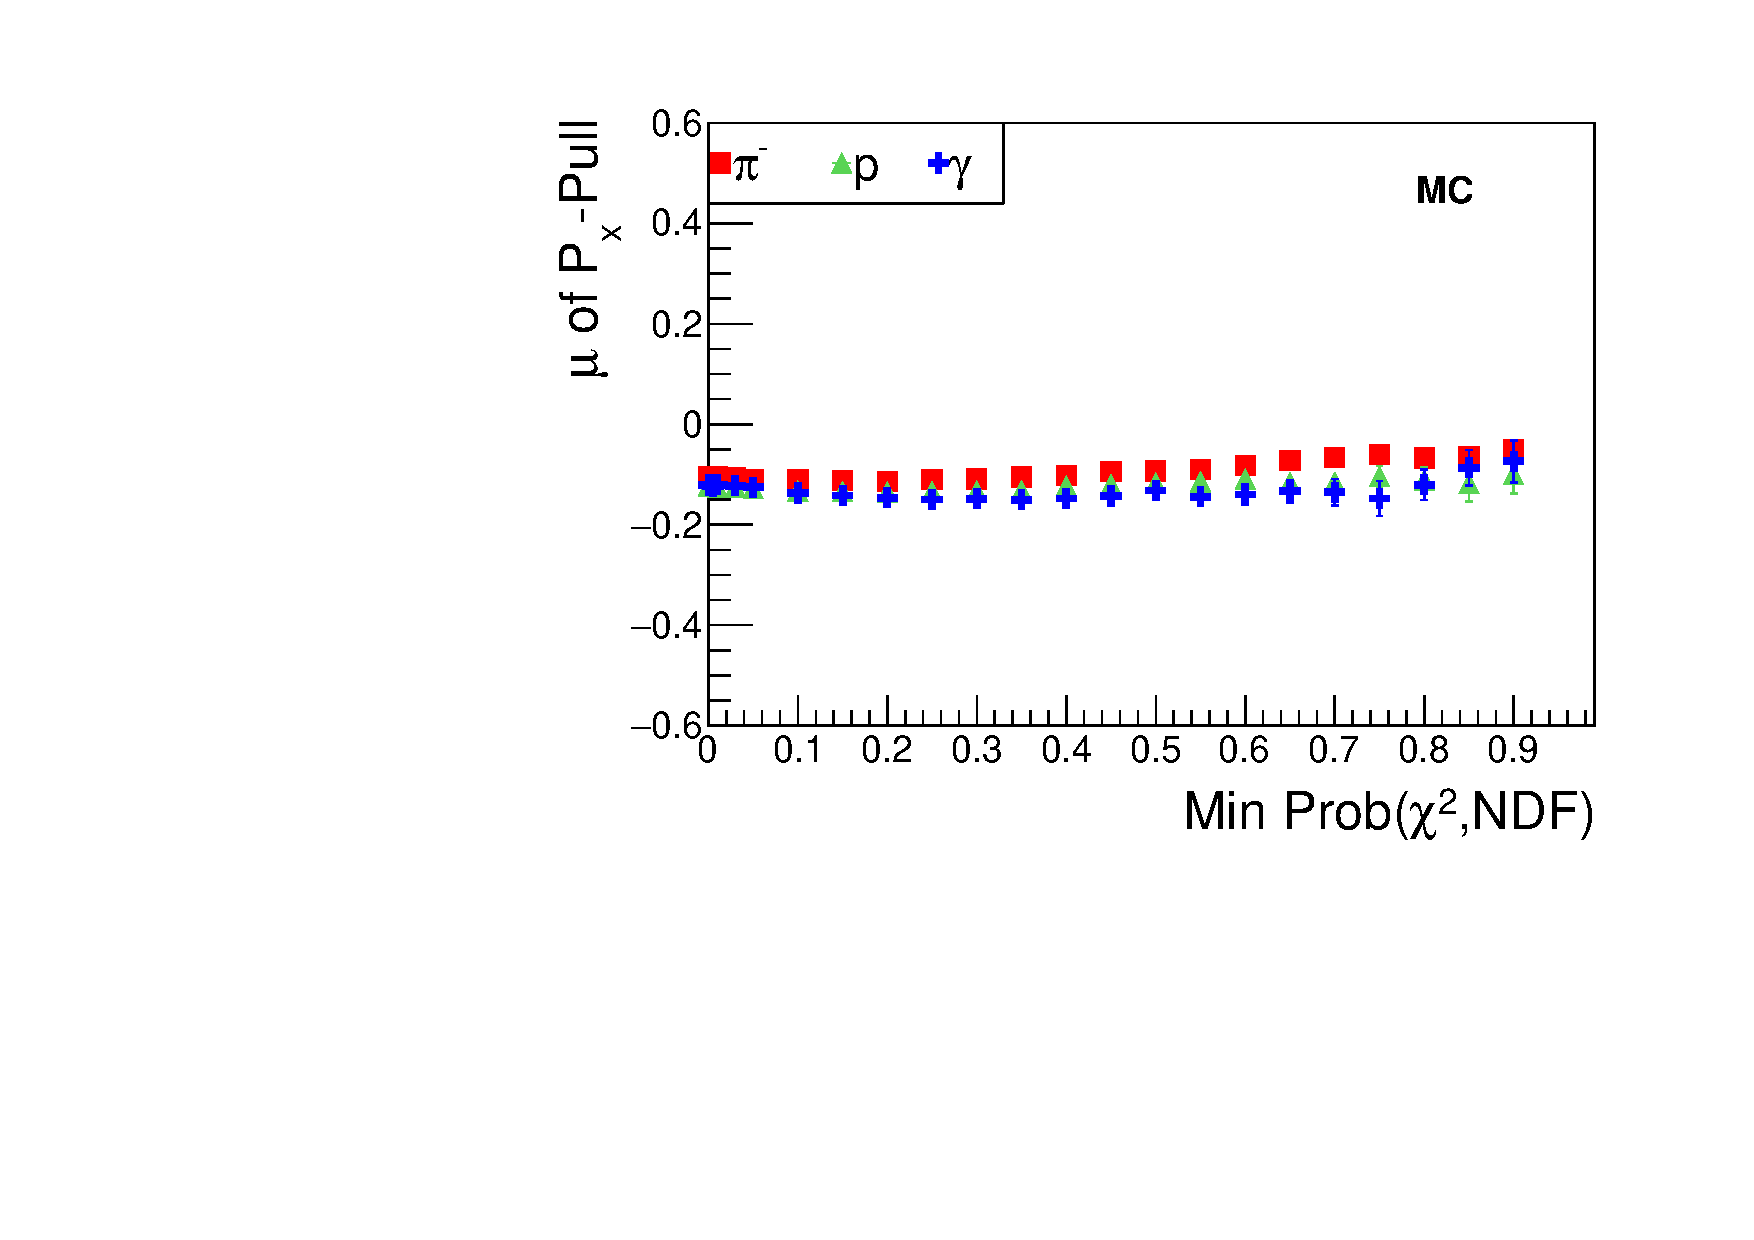
\includegraphics[width=0.3\textwidth]{figures/gluex_nim_pullspx_pulls_mean_mc.pdf}
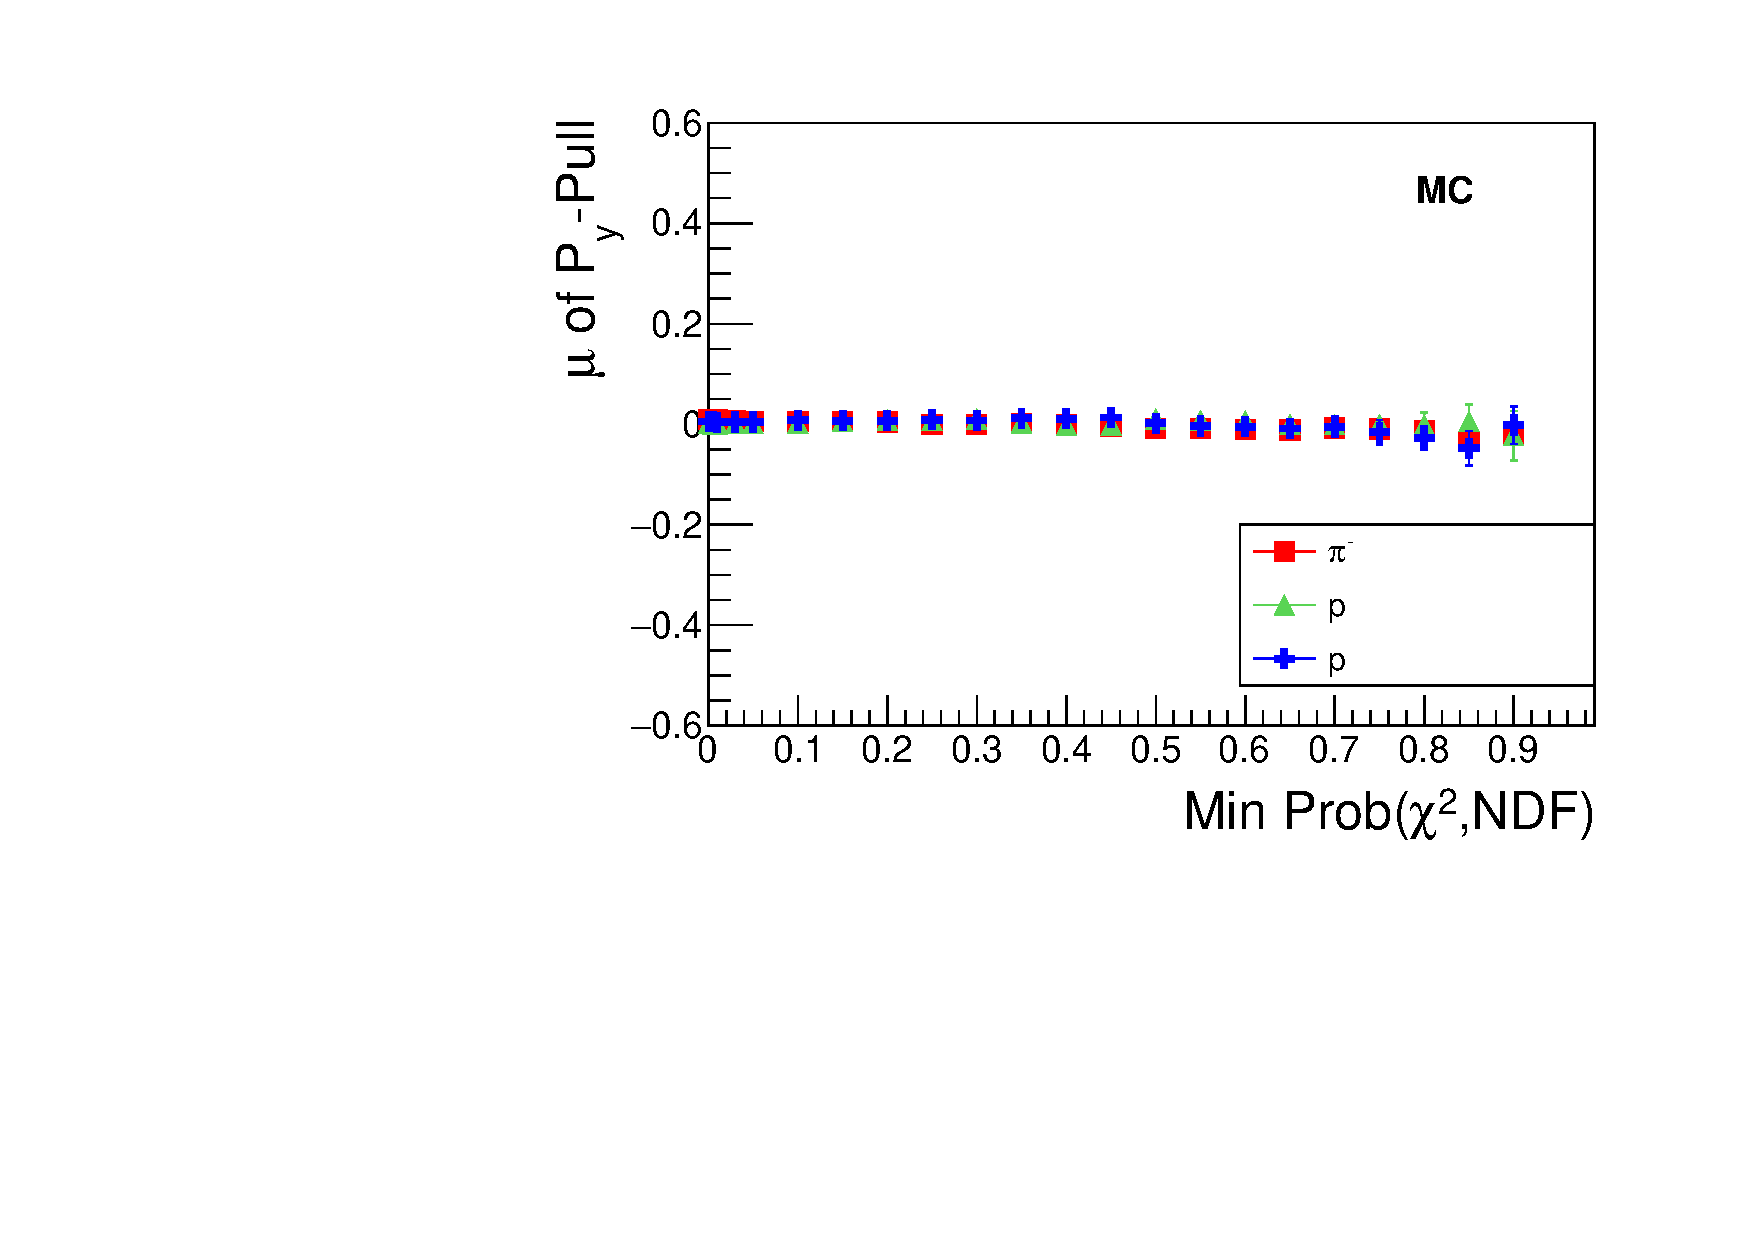
\includegraphics[width=0.3\textwidth]{figures/gluex_nim_pullspy_pulls_mean_mc.pdf}
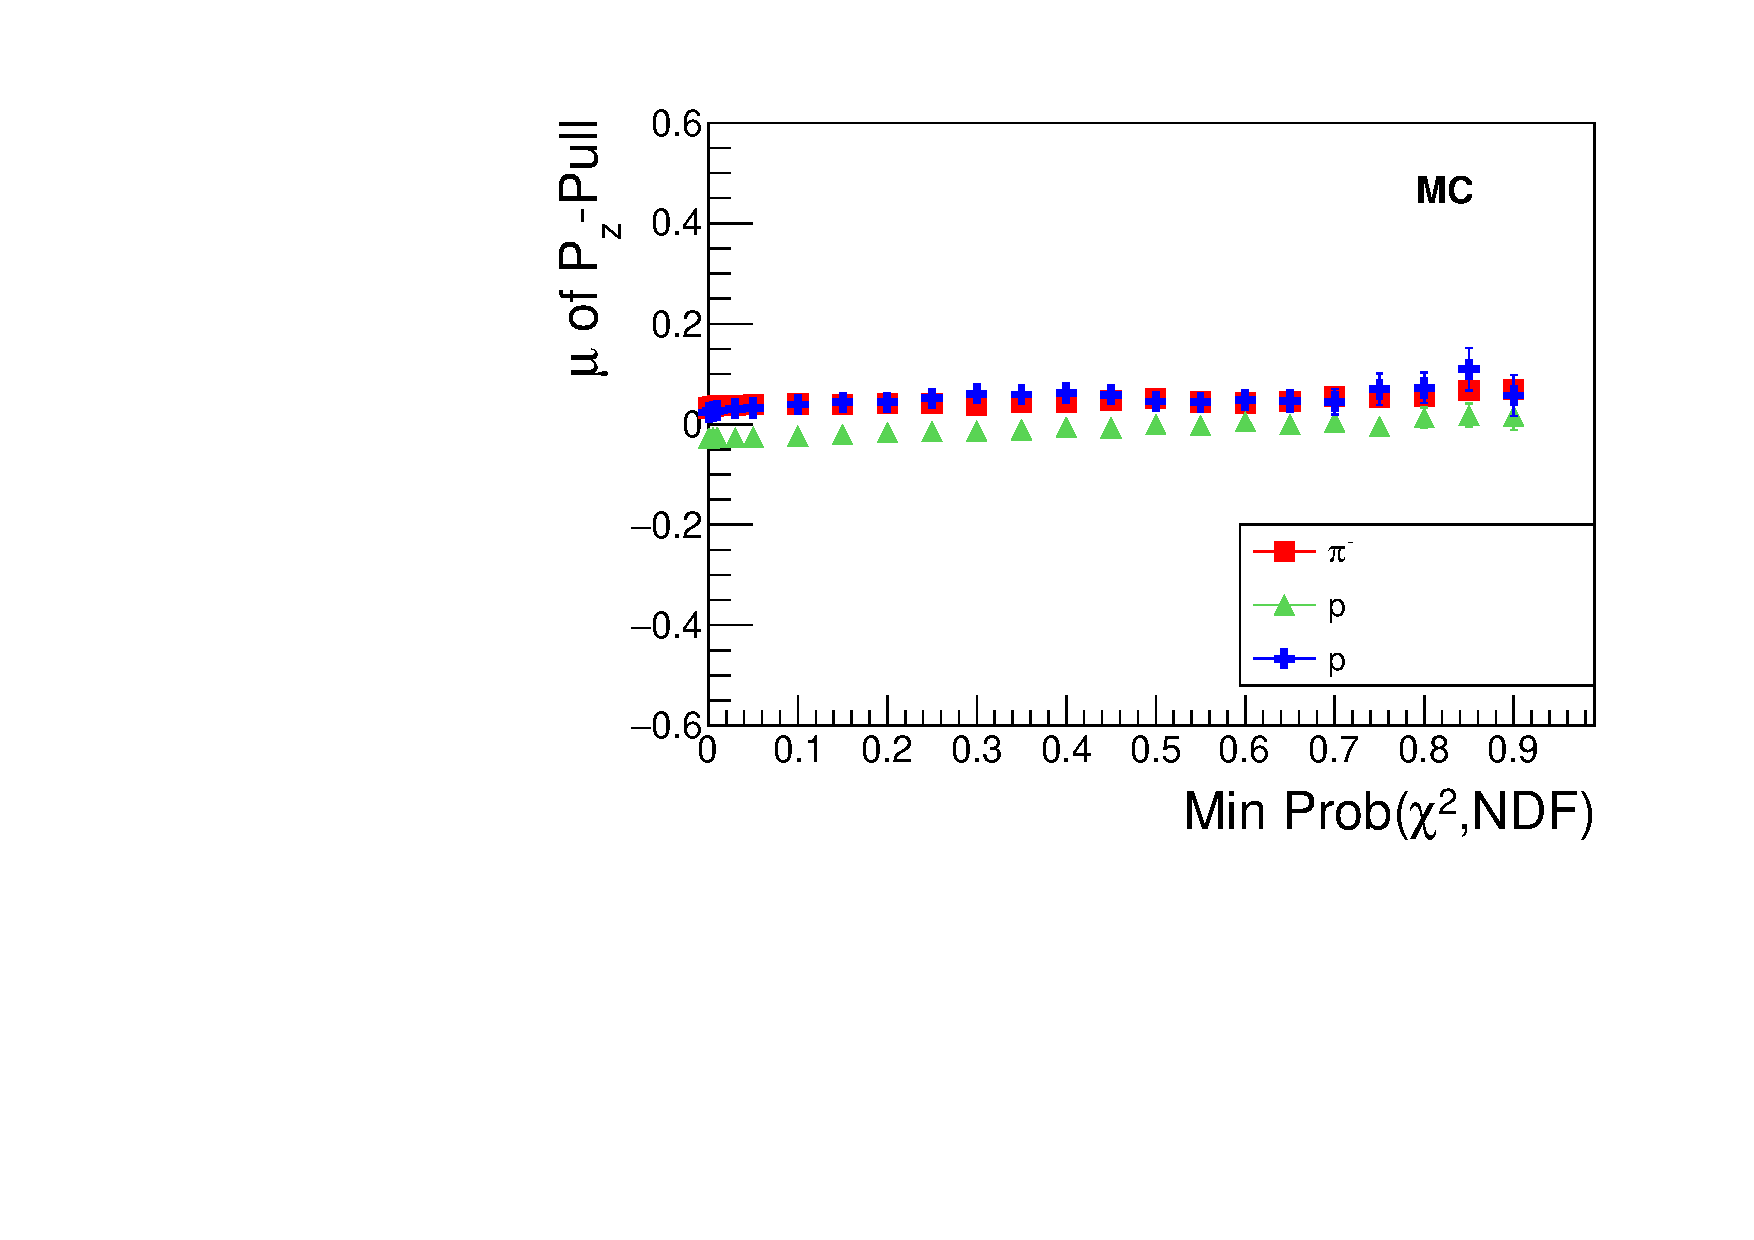
\includegraphics[width=0.3\textwidth]{figures/gluex_nim_pullspz_pulls_mean_mc.pdf}

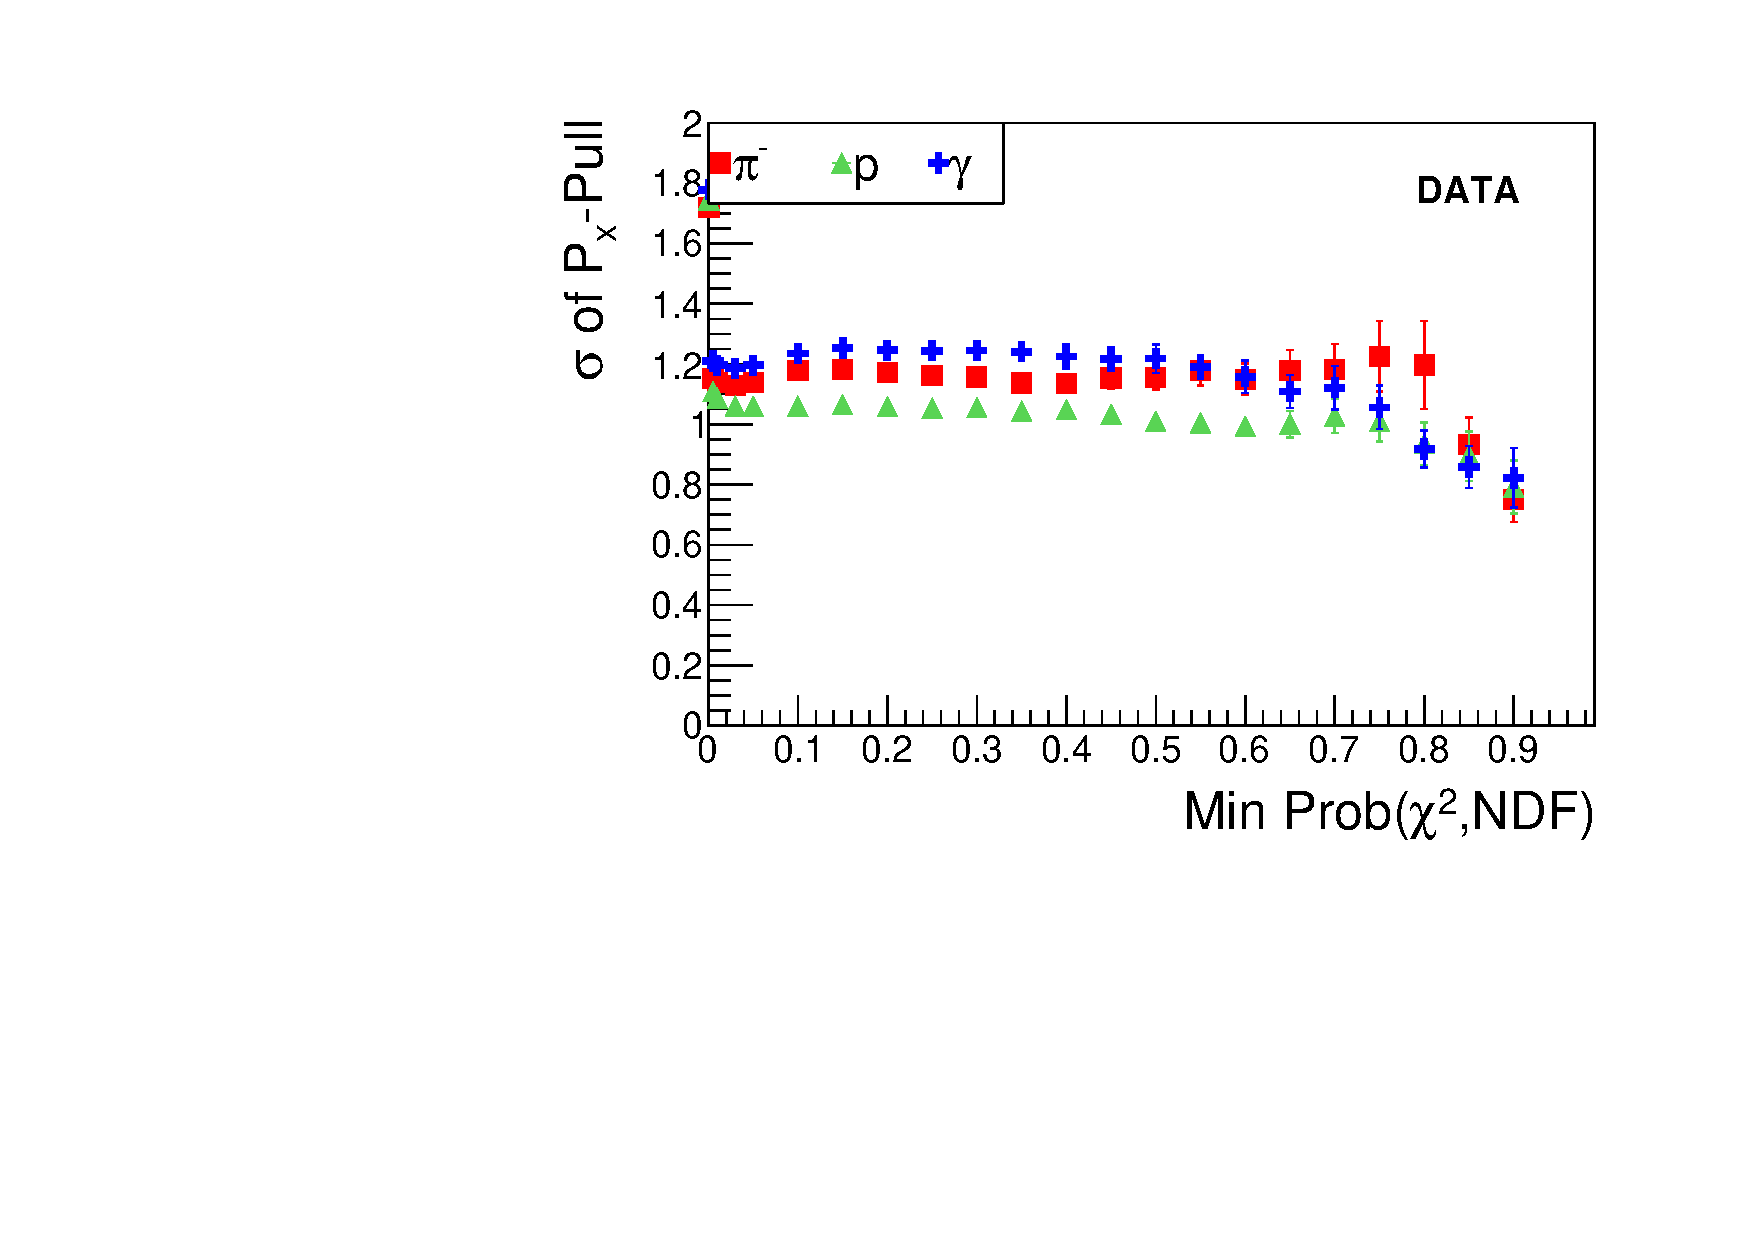
\includegraphics[width=0.3\textwidth]{figures/gluex_nim_pullspx_pulls_sigma_data.pdf}
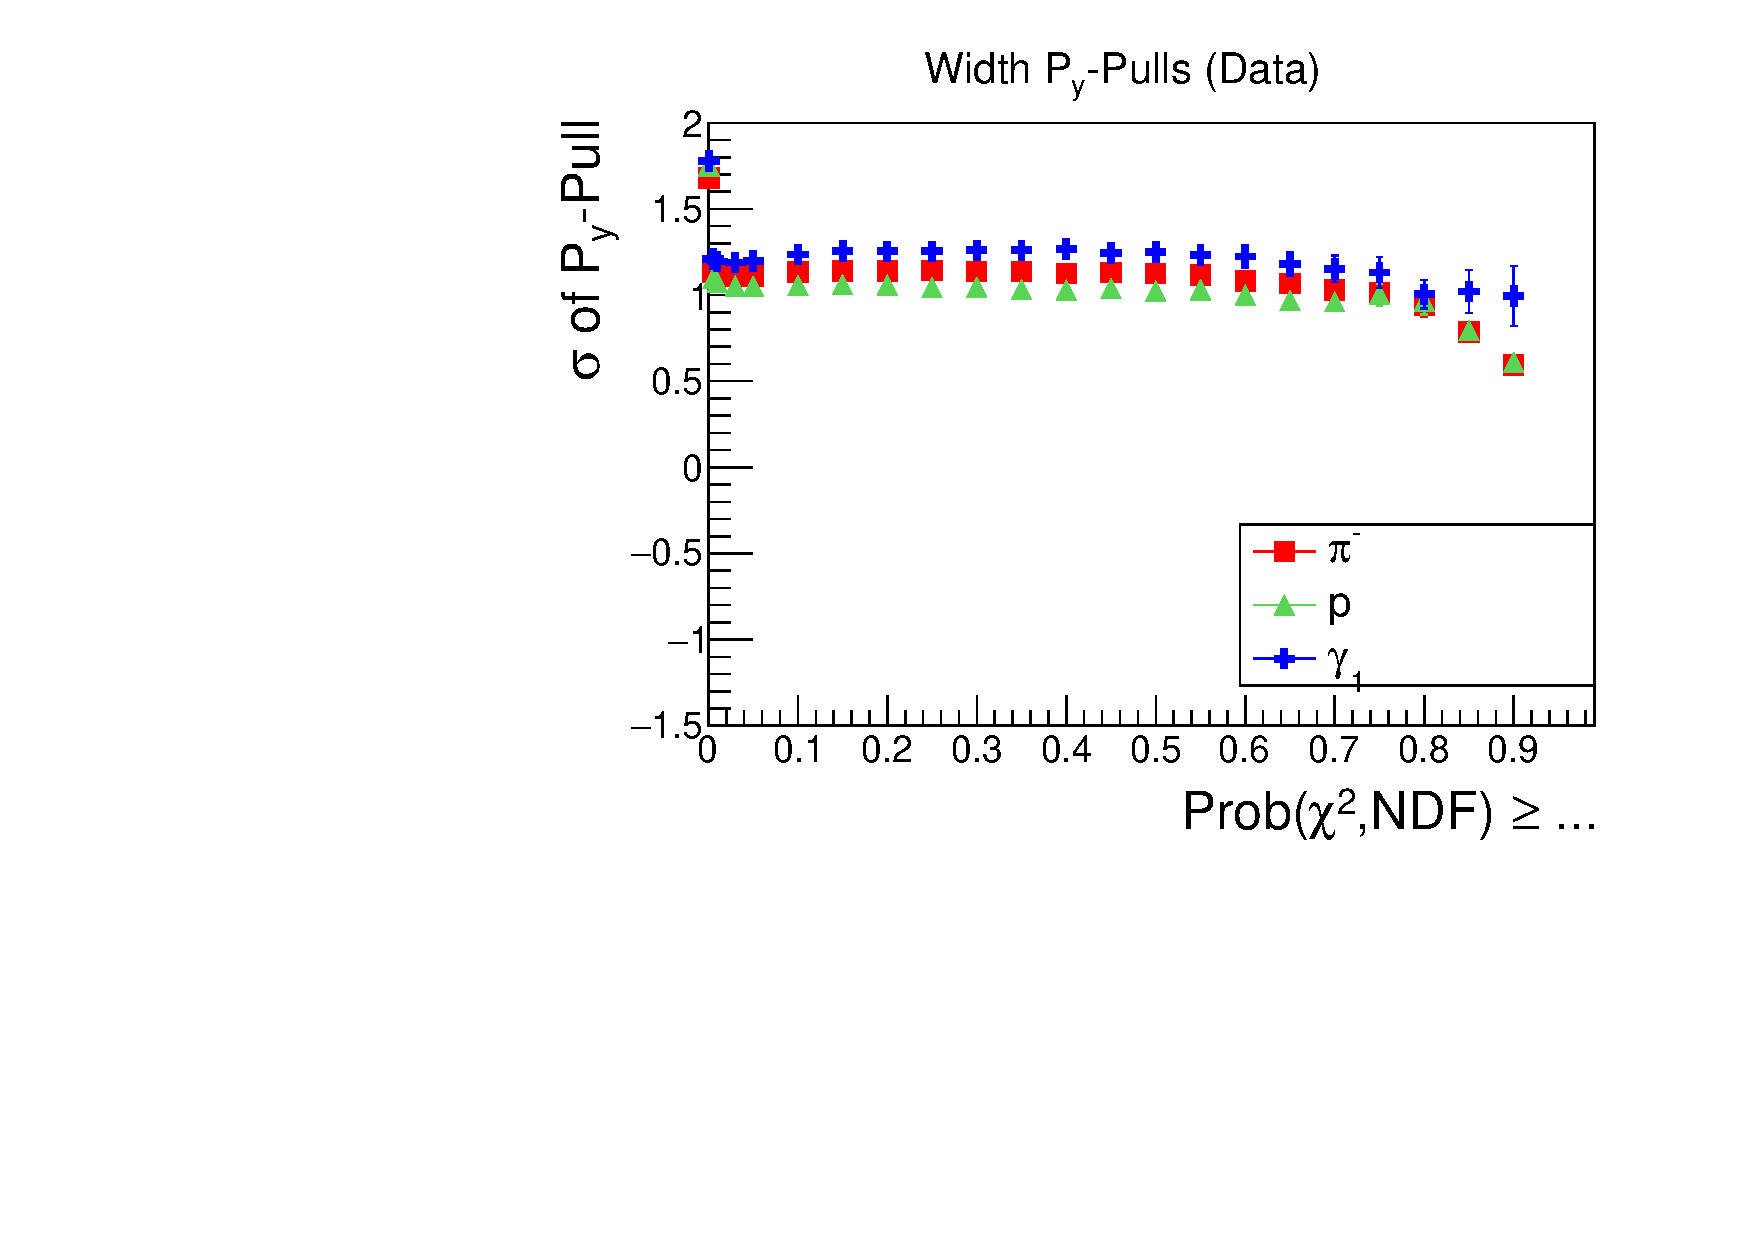
\includegraphics[width=0.3\textwidth]{figures/gluex_nim_pullspy_pulls_sigma_data.pdf}
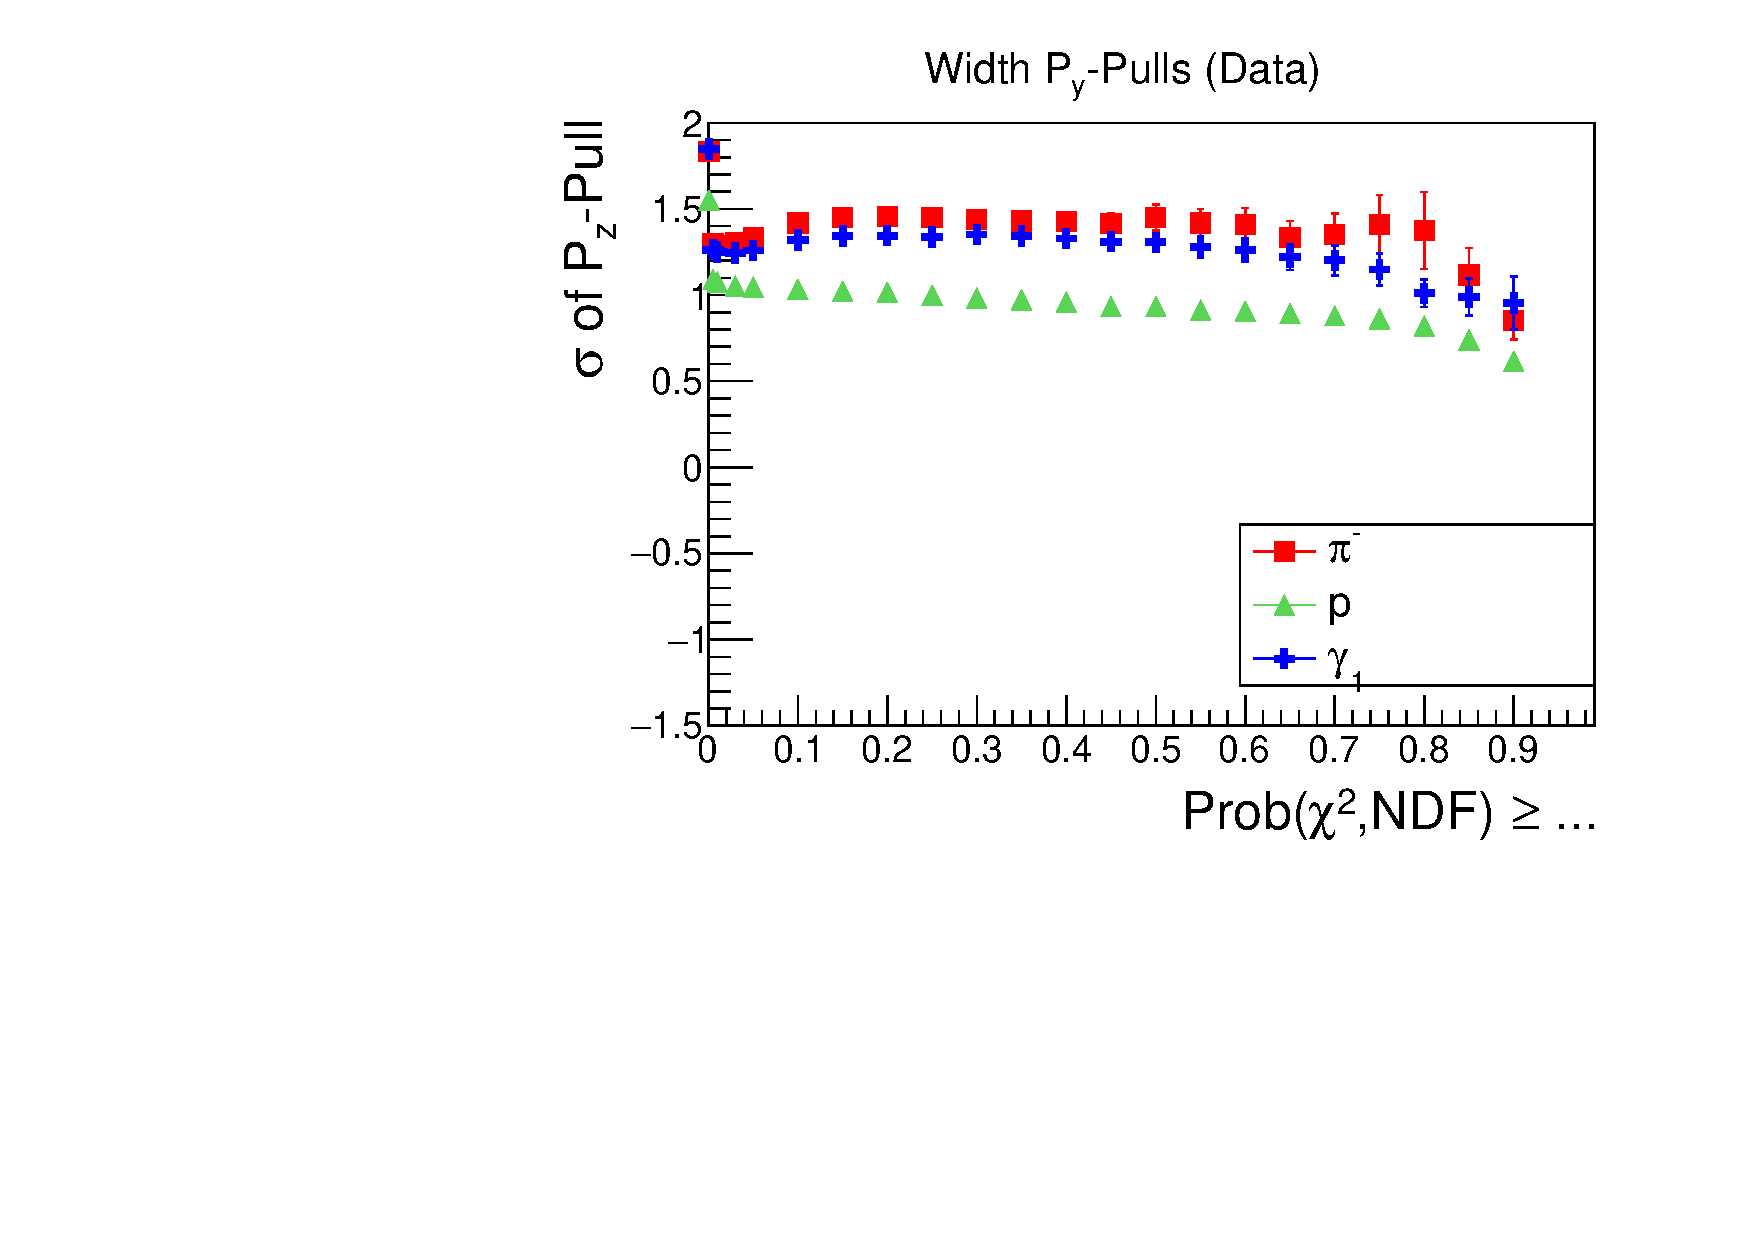
\includegraphics[width=0.3\textwidth]{figures/gluex_nim_pullspz_pulls_sigma_data.pdf}

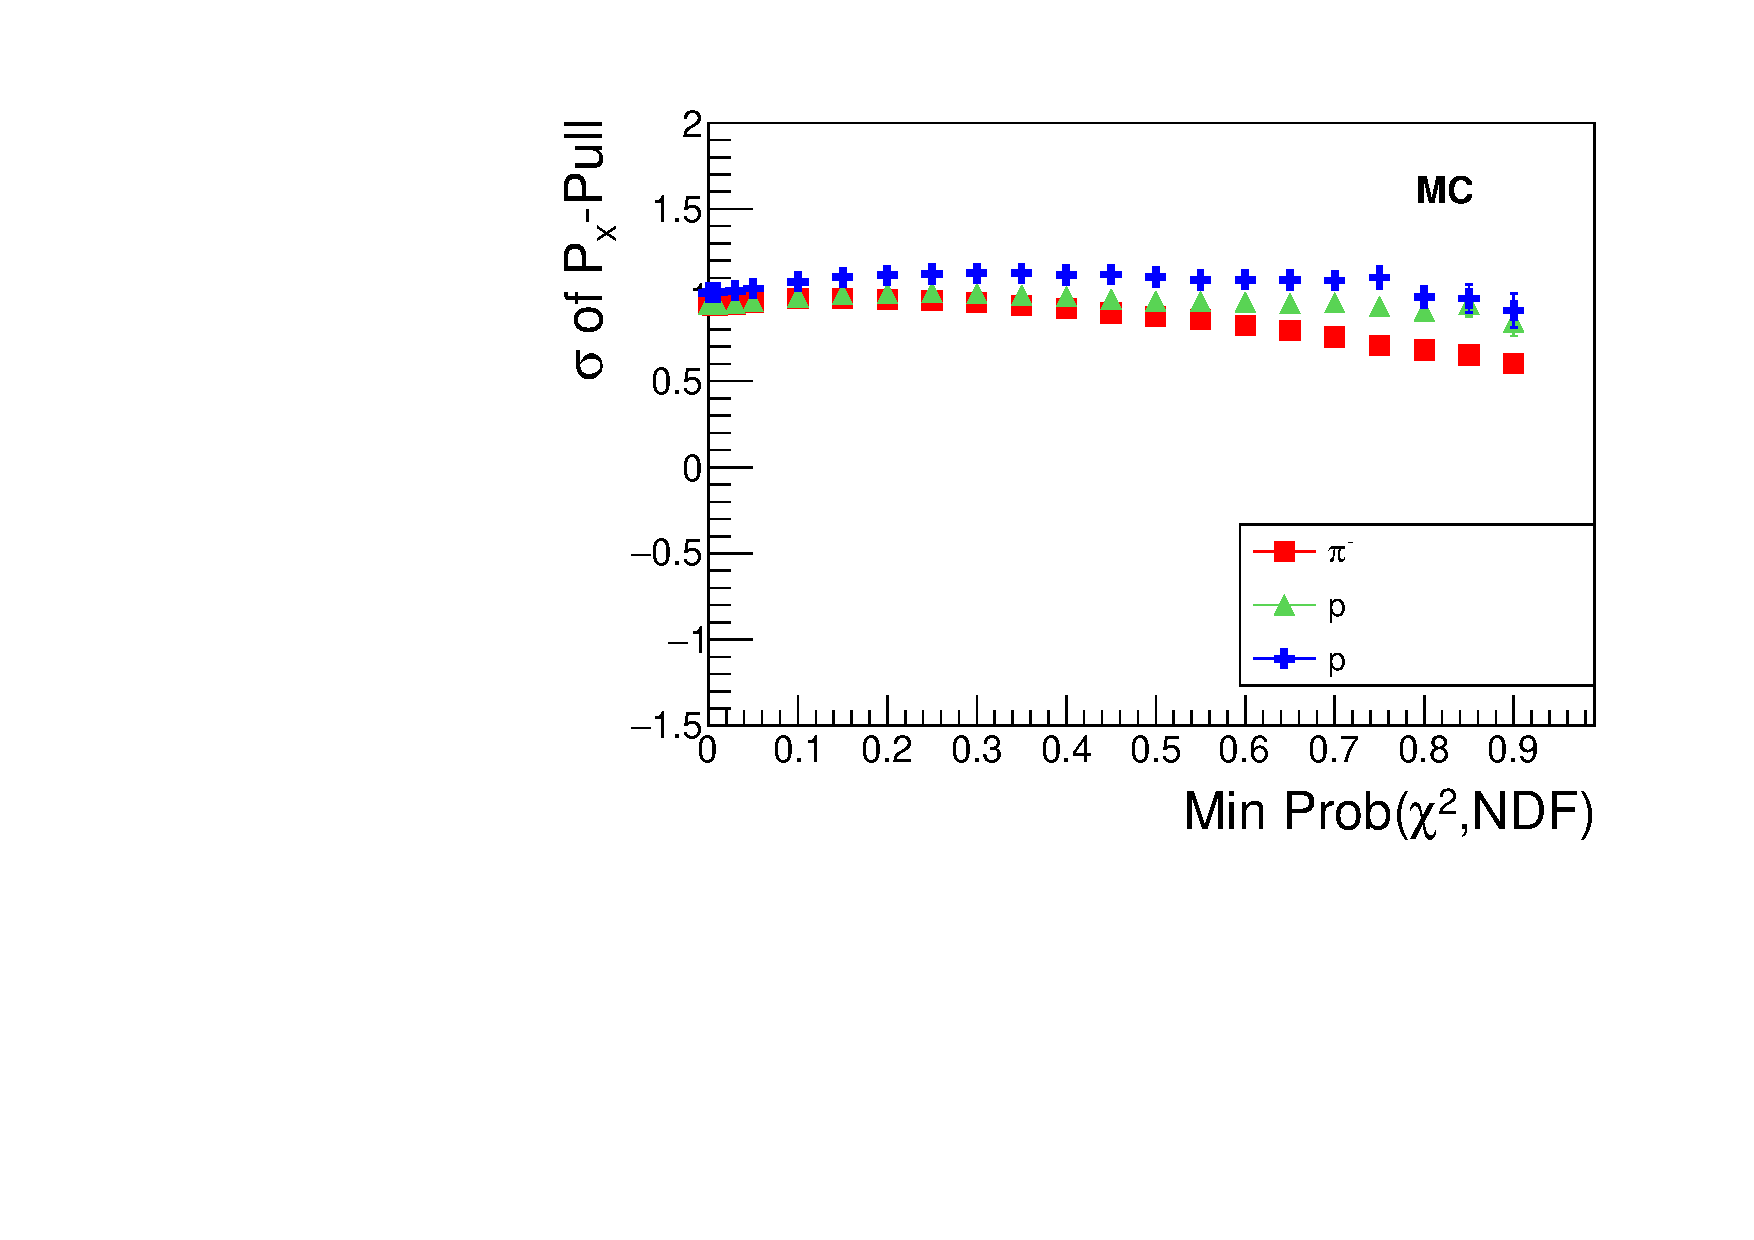
\includegraphics[width=0.3\textwidth]{figures/gluex_nim_pullspx_pulls_sigma_mc.pdf}
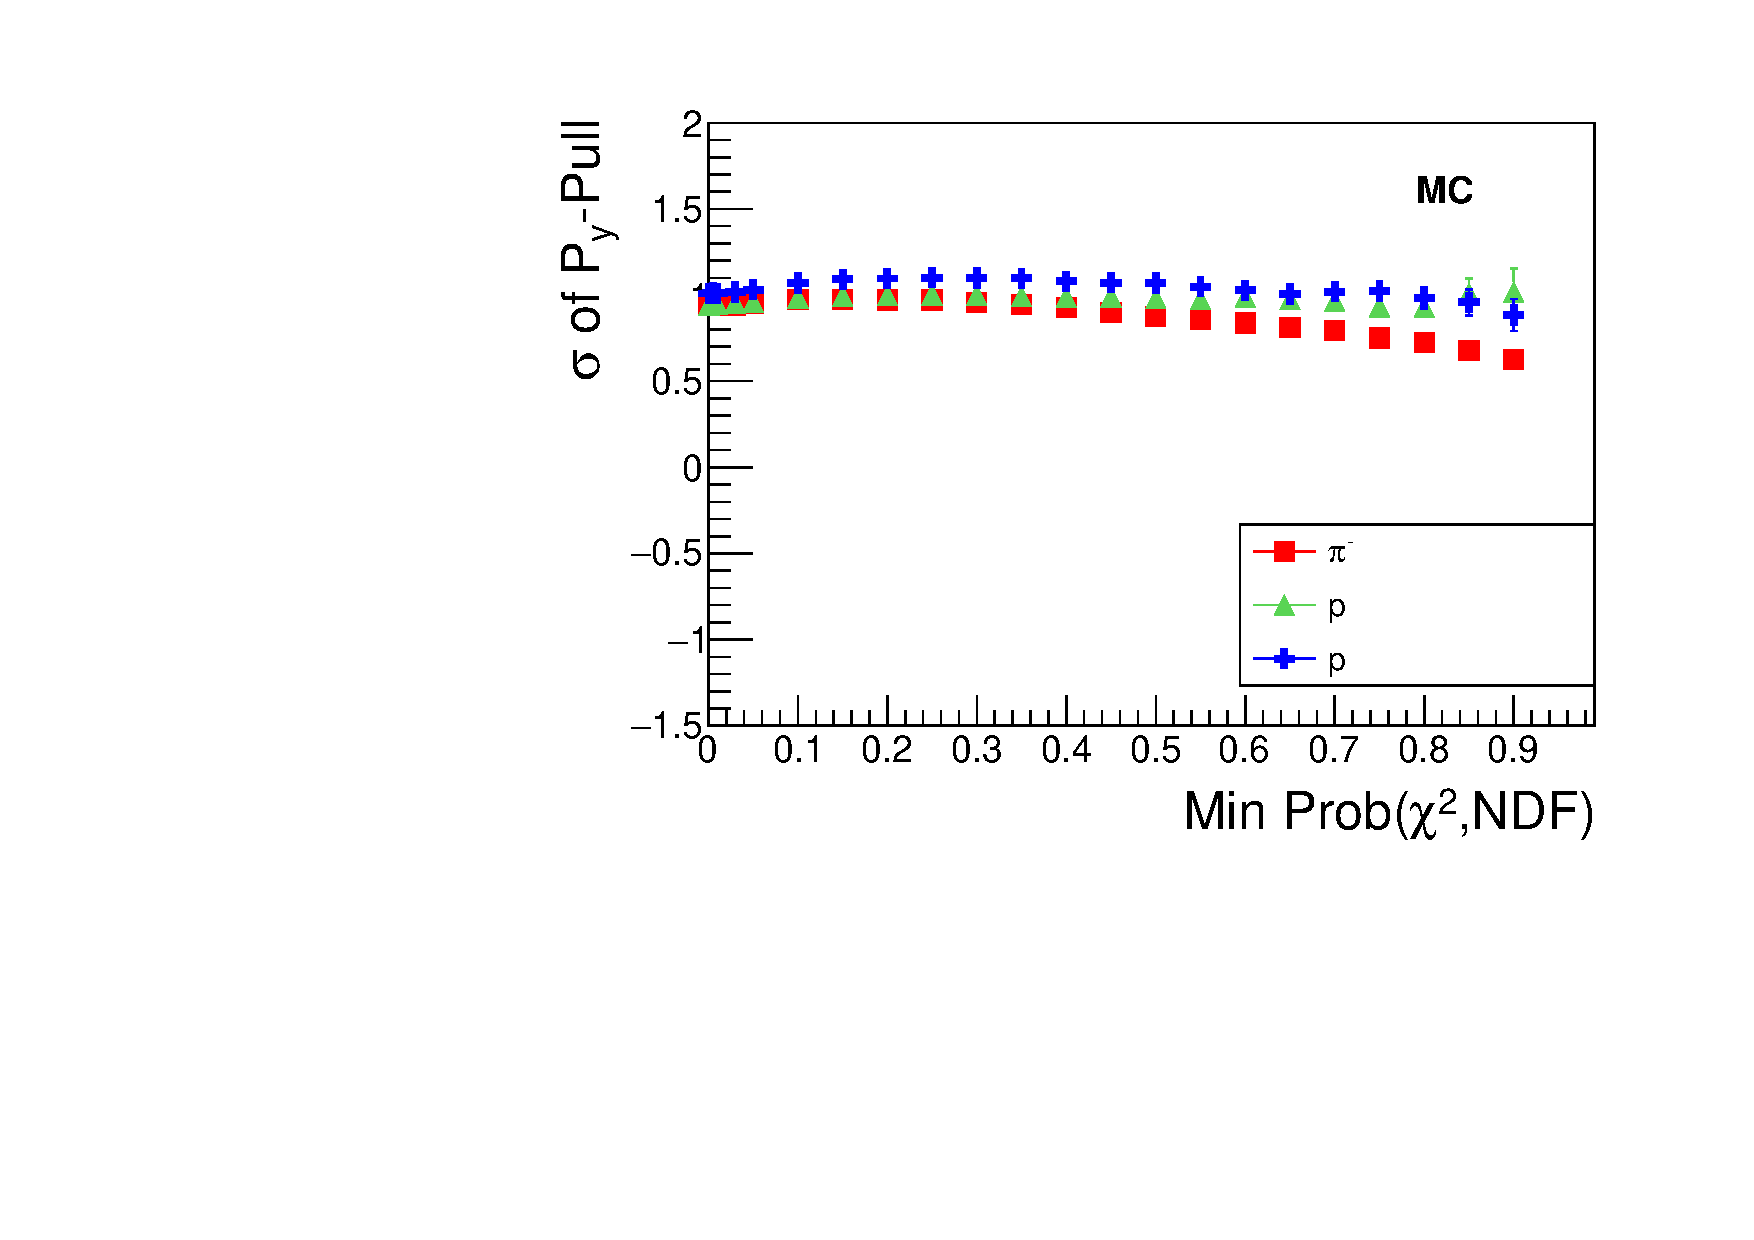
\includegraphics[width=0.3\textwidth]{figures/gluex_nim_pullspy_pulls_sigma_mc.pdf}
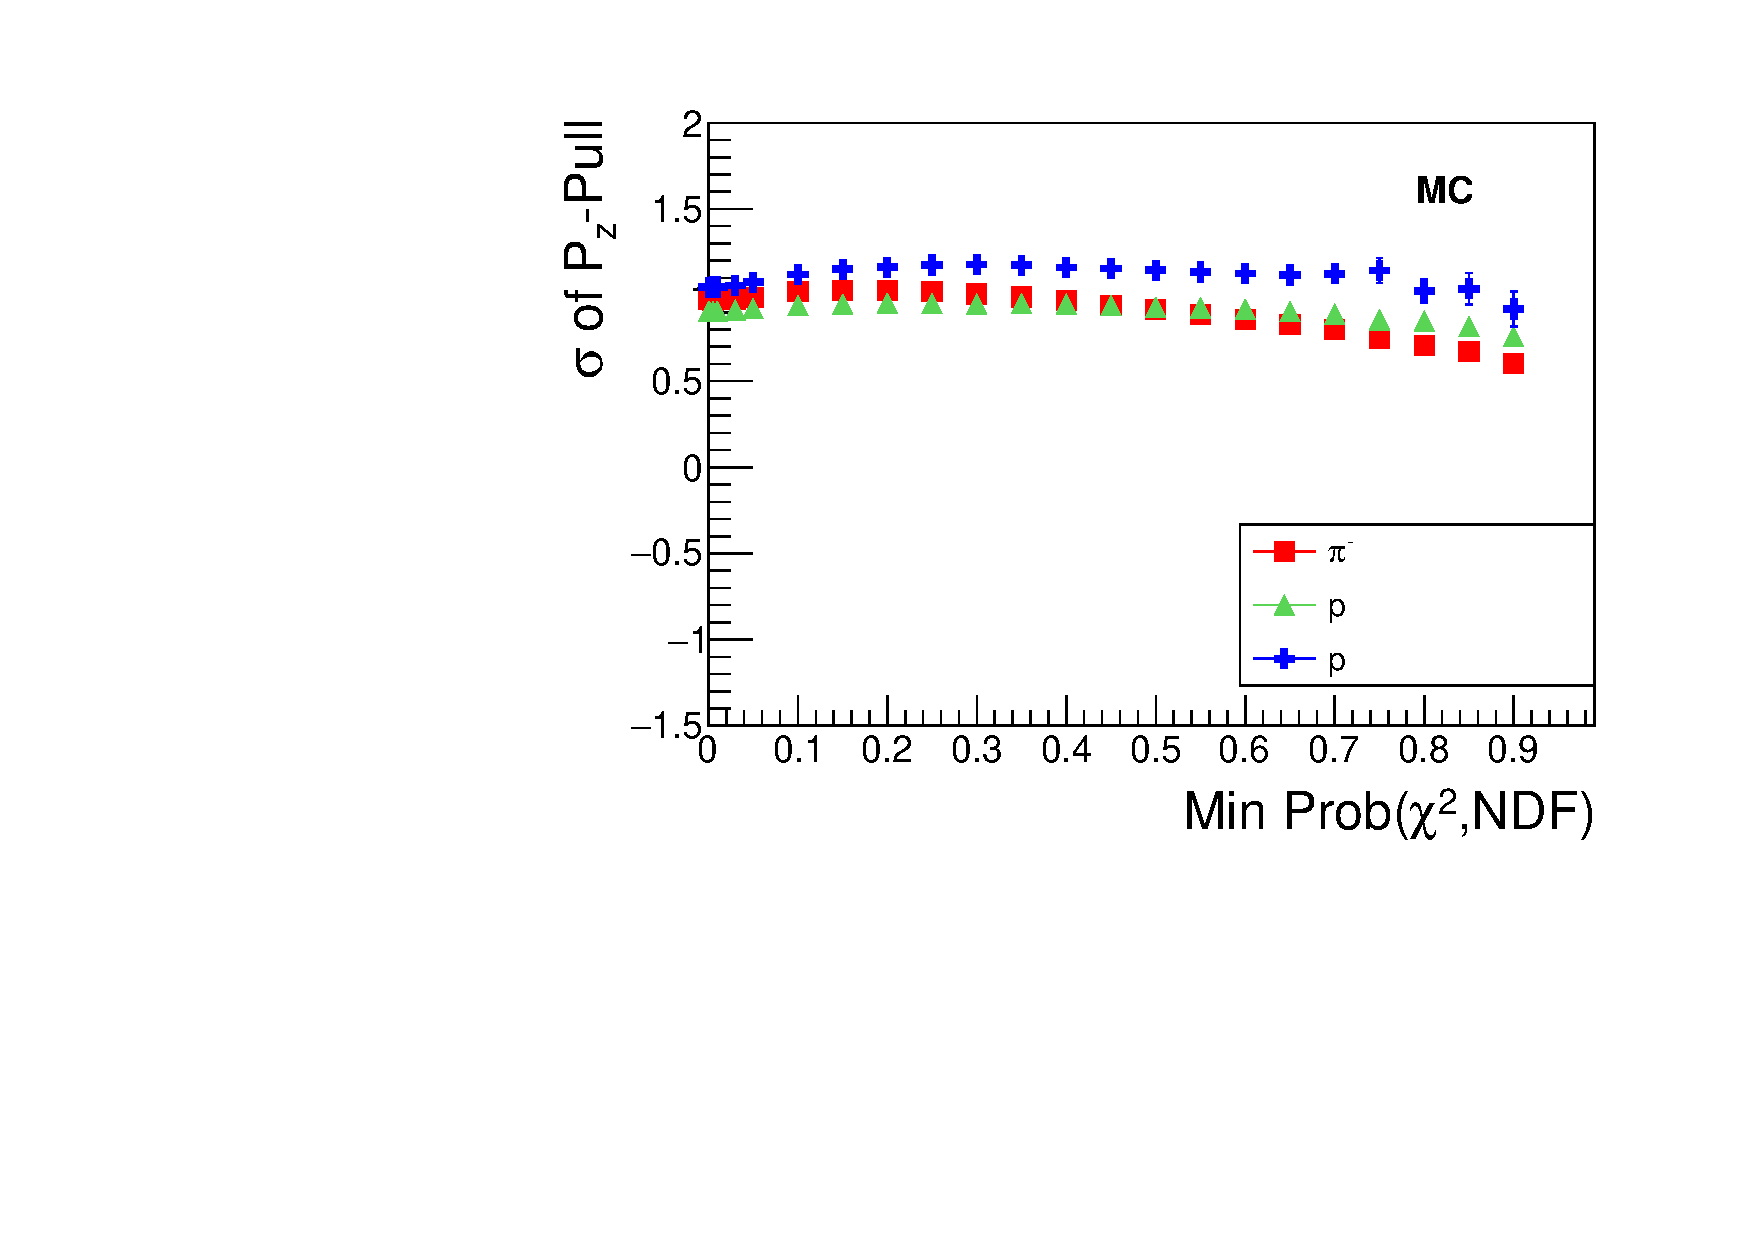
\includegraphics[width=0.3\textwidth]{figures/gluex_nim_pullspz_pulls_sigma_mc.pdf}

\caption{\label{fig:kinfitstudy}
Pull means (top) and sigmas (bottom) for the momentum components of each particle as a function of the minimum probability required of the fit from reconstructed $\gamma p \to \eta p$,  $\eta \to \pi^+\pi^-\pi^0$ events.
 (Color online)}
\end{center}  
\end{figure}

\subsection{Invariant-mass resolution \label{sec:perfchargedresol}}

The invariant-mass resolution for resonances depends on the momenta and angles of their decay products.  This resolution has been studied using several different channels, which are illustrated in Figs.~\ref{fig:invmass1} and \ref{fig:invmass2}. A typical meson production channel including both charged particles and photons, $\omega \to \pi^+\pi^-\pi^0$ from $\gamma p \to \omega p$, is shown in the left panel of Fig.~\ref{fig:invmass1}. The distribution shows the strong peak due to $\omega$ meson production.  Other structures are also seen, such as peaks corresponding to the production of $\eta$ and $\phi$ mesons.  The $\omega$ peak resolution obtained is 26.1~MeV when using only the reconstructed  particle 4-vectors, and improves to 16.4~MeV after a kinematic fit. The invariant-mass distribution of $\pi^+\pi^-$ from $\gamma p \to K_S K^+ \pi^- p$, $K_S\to\pi^+\pi^-$ exhibits the peak due to $K_S\to\pi^+\pi^-$ decays (right panel of Fig.\,\ref{fig:invmass1}).  The $K_S$ peak resolution is 17.0~MeV using only the reconstructed charged particle 4-vectors, and improves to  8.6~MeV after a kinematic fit imposing energy and momentum conservation. The dependence of the $K_S\to\pi^+\pi^-$ invariant-mass resolution as a function of $K_S$ momentum is shown in Fig.\,\ref{fig:invmass1a} , both before and after an energy/momentum-constraint kinematic fit.  

The invariant mass of $\Lambda^0\pi^-$ from $\gamma p \to K^+ K^+ \pi^- \pi^- p$ is shown in the left panel of Fig.\,\ref{fig:invmass2},  illustrating the peak due to $\Xi^- \to \pi^- \Lambda^0$, $\Lambda^0 \to p \pi^-$.  The $\Xi^-$ peak resolution obtained is 7.3~MeV when using only the reconstructed charged particle 4-vectors, and improves to 4.6~MeV after a kinematic fit imposing energy and momentum conservation and the additional constraint that the mass of the $p \pi^-$ pairs must be that of the $\Lambda^0$ mass.  The $e^+e^-$ invariant mass distribution from kinematically fit $\gamma p \to e^+e^- p$ events is shown in the right panel of Fig.\,\ref{fig:invmass2}, illustrating the peak due to $J/\psi\to e^+e^-$.  The resolution of the peak is 13.7~MeV.          

\begin{figure}[tpb]
\begin{center}
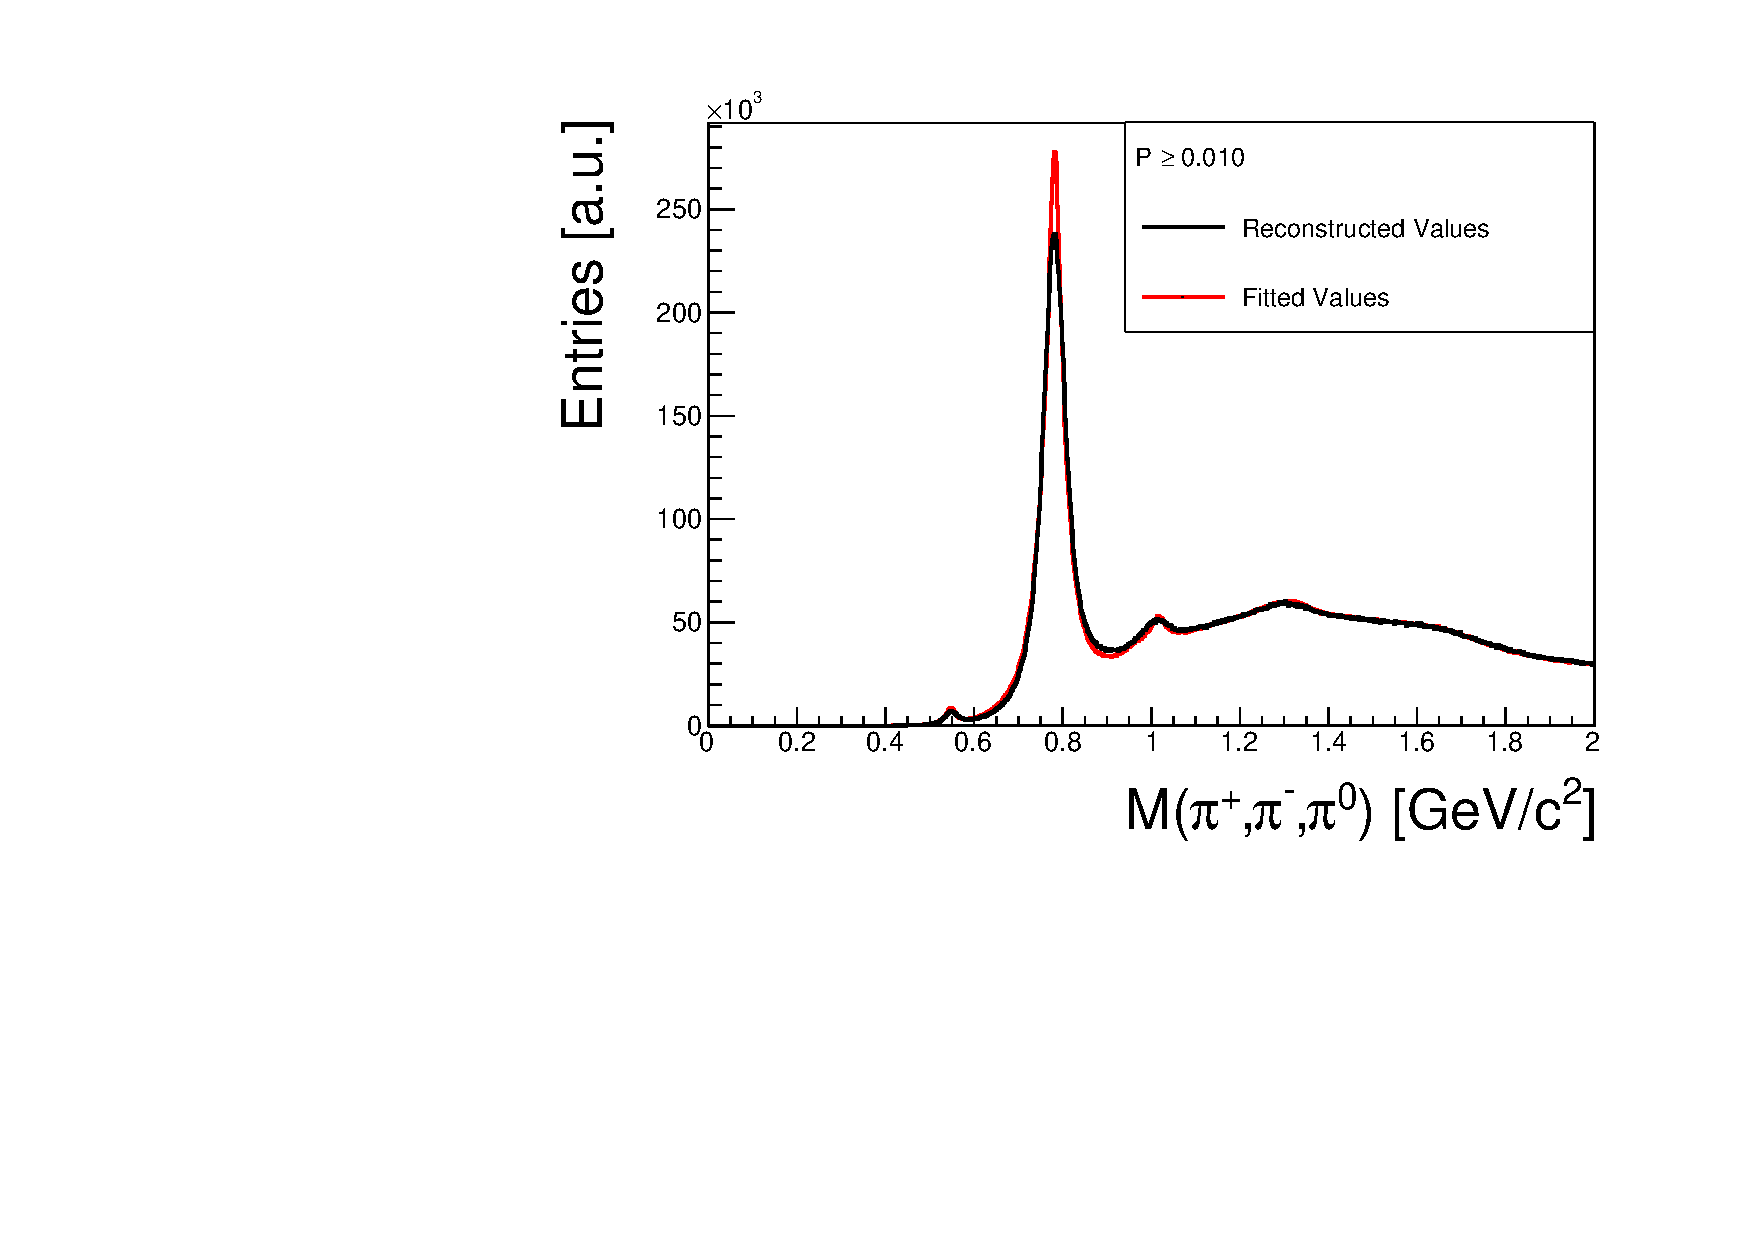
\includegraphics[width=0.45\textwidth]{figures/omega_inv_mass_probCut_001.pdf}
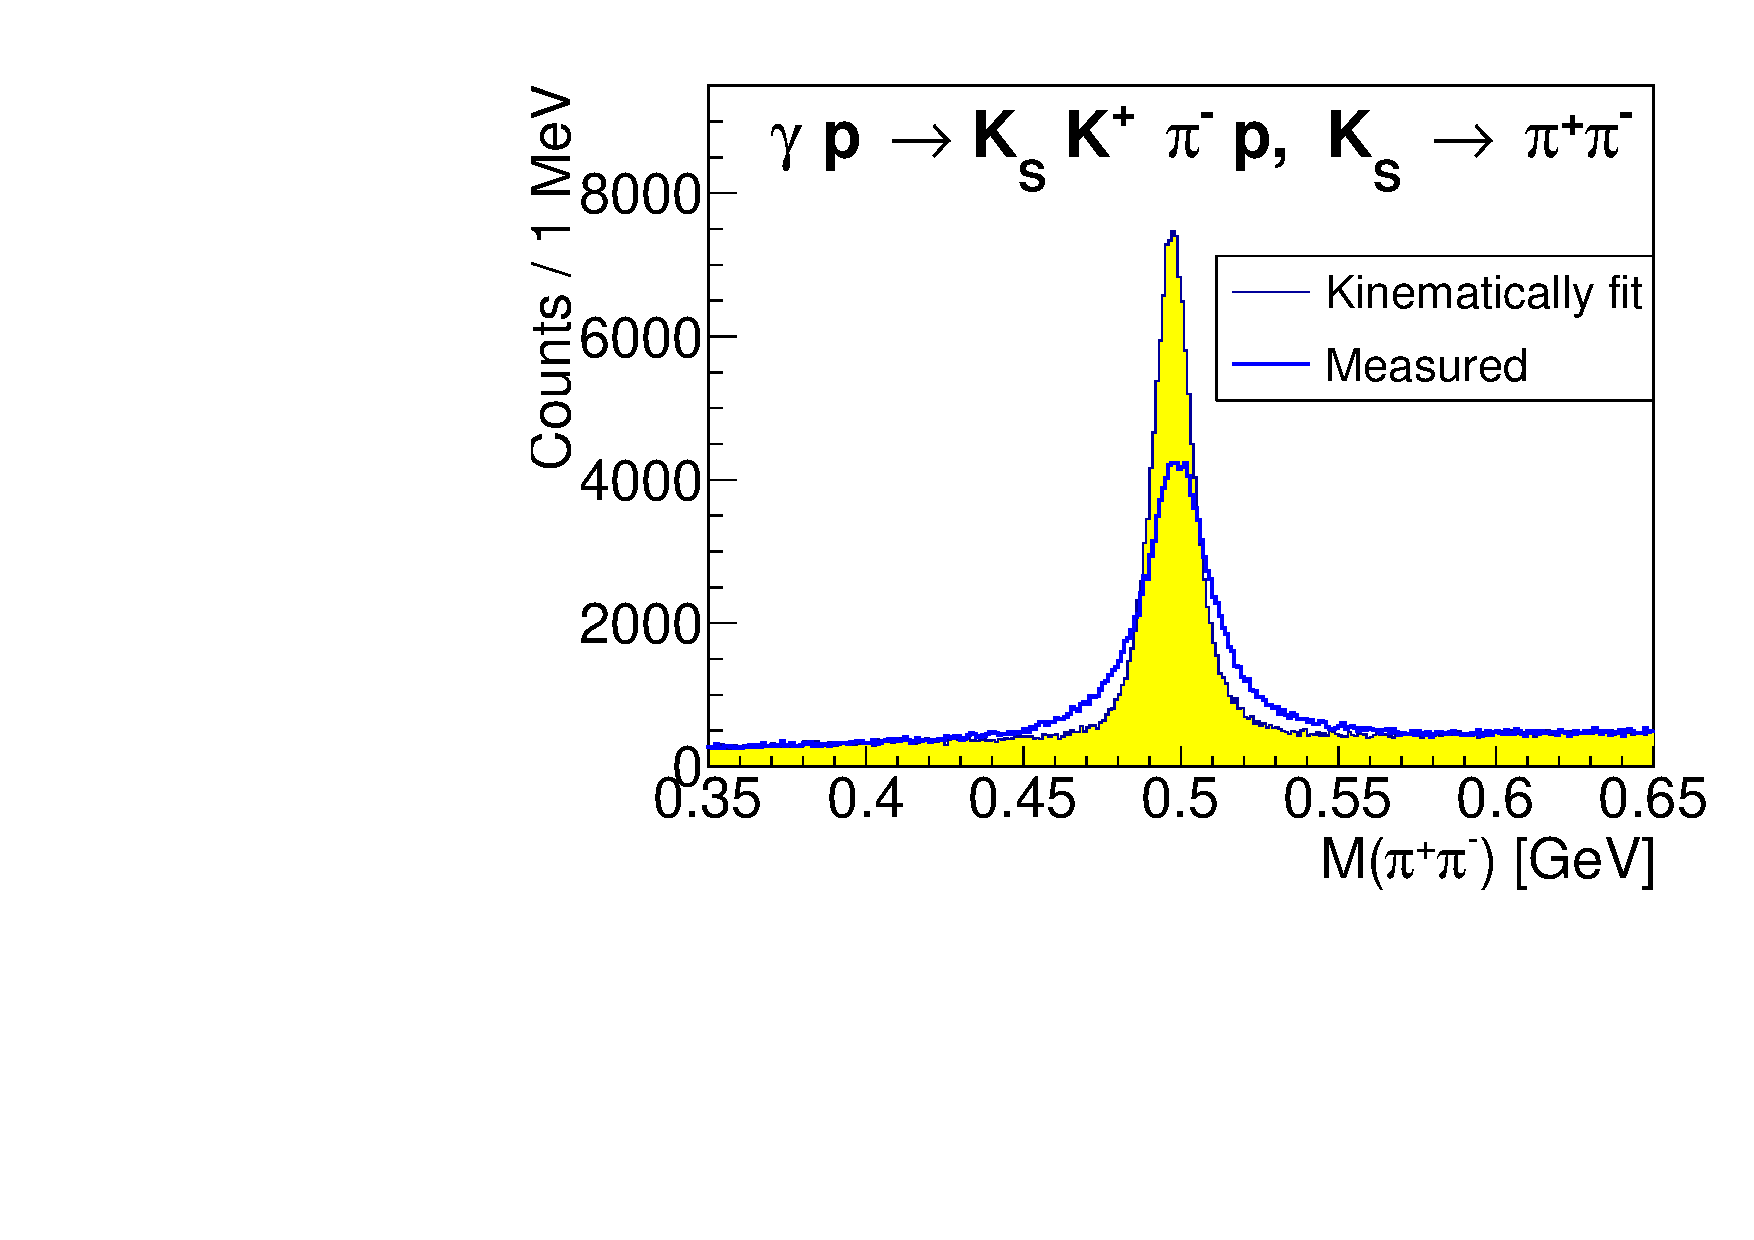
\includegraphics[width=0.4\textwidth]{figures/kskpi_mass_spect.pdf}
\caption{\label{fig:invmass1}
(Left top) $\pi^+\pi^-\pi^0$ invariant-mass distribution from $\gamma p \to \pi^+\pi^-\pi^0 p$ (Right top) $\pi^+\pi^-$ invariant mass distribution from $\gamma p \to K_S K^+ \pi^- p$, $K_S\to\pi^+\pi^-$. (Color online)}
\end{center}
\end{figure}


\begin{figure}[tpb]
\begin{center}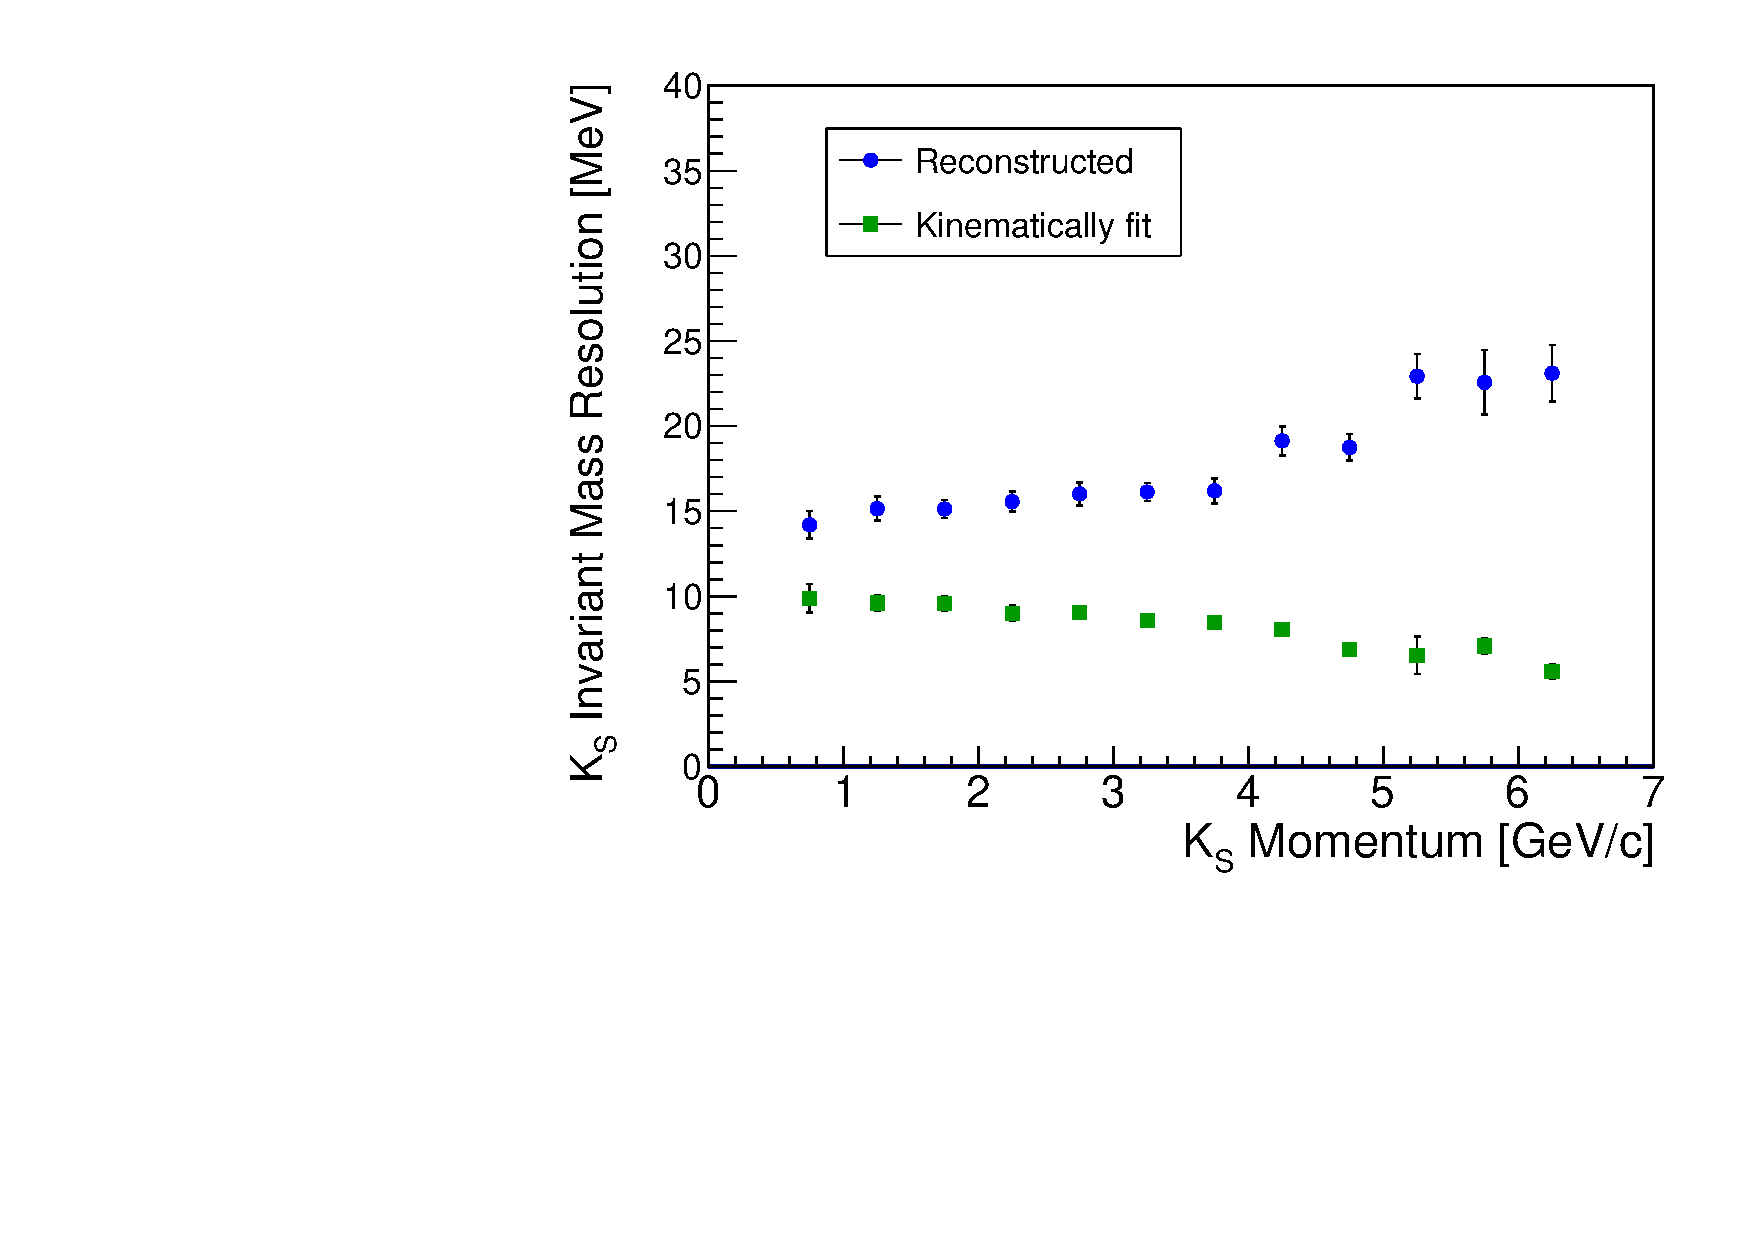
\includegraphics[width=0.5\textwidth]{figures/kskpi_mass_resol.pdf}
\caption{\label{fig:invmass1a}
$K_S\to\pi^+\pi^-$ invariant mass resolution for the events shown in Fig.\,\ref{fig:invmass1}, as a function of $K_S$ momentum, both before and after a kinetic fit, which constrains energy and momentum conservation.  
(Color online)}
\end{center}
\end{figure}


\begin{figure}[tpb]
\begin{center}
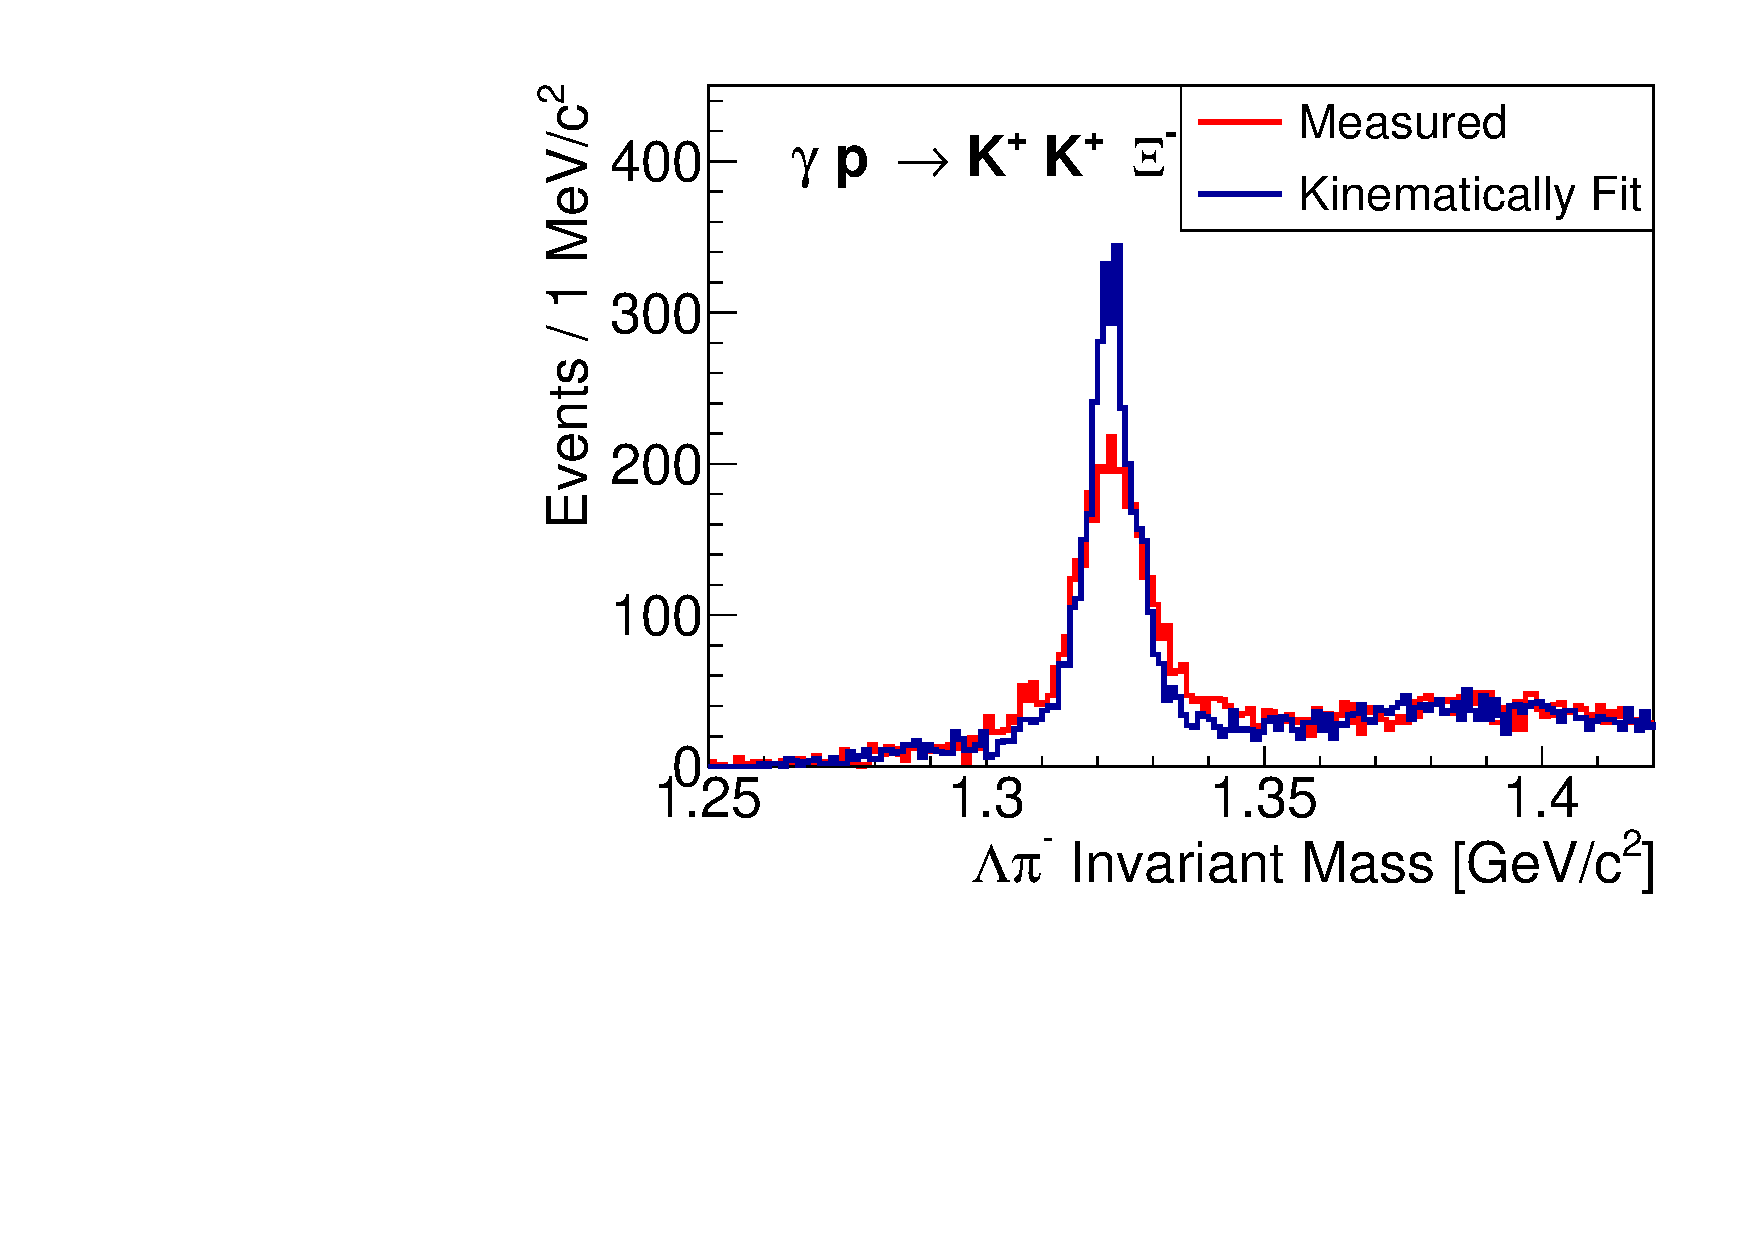
\includegraphics[width=0.42\textwidth]{figures/XimMass_2017-ver30.pdf}
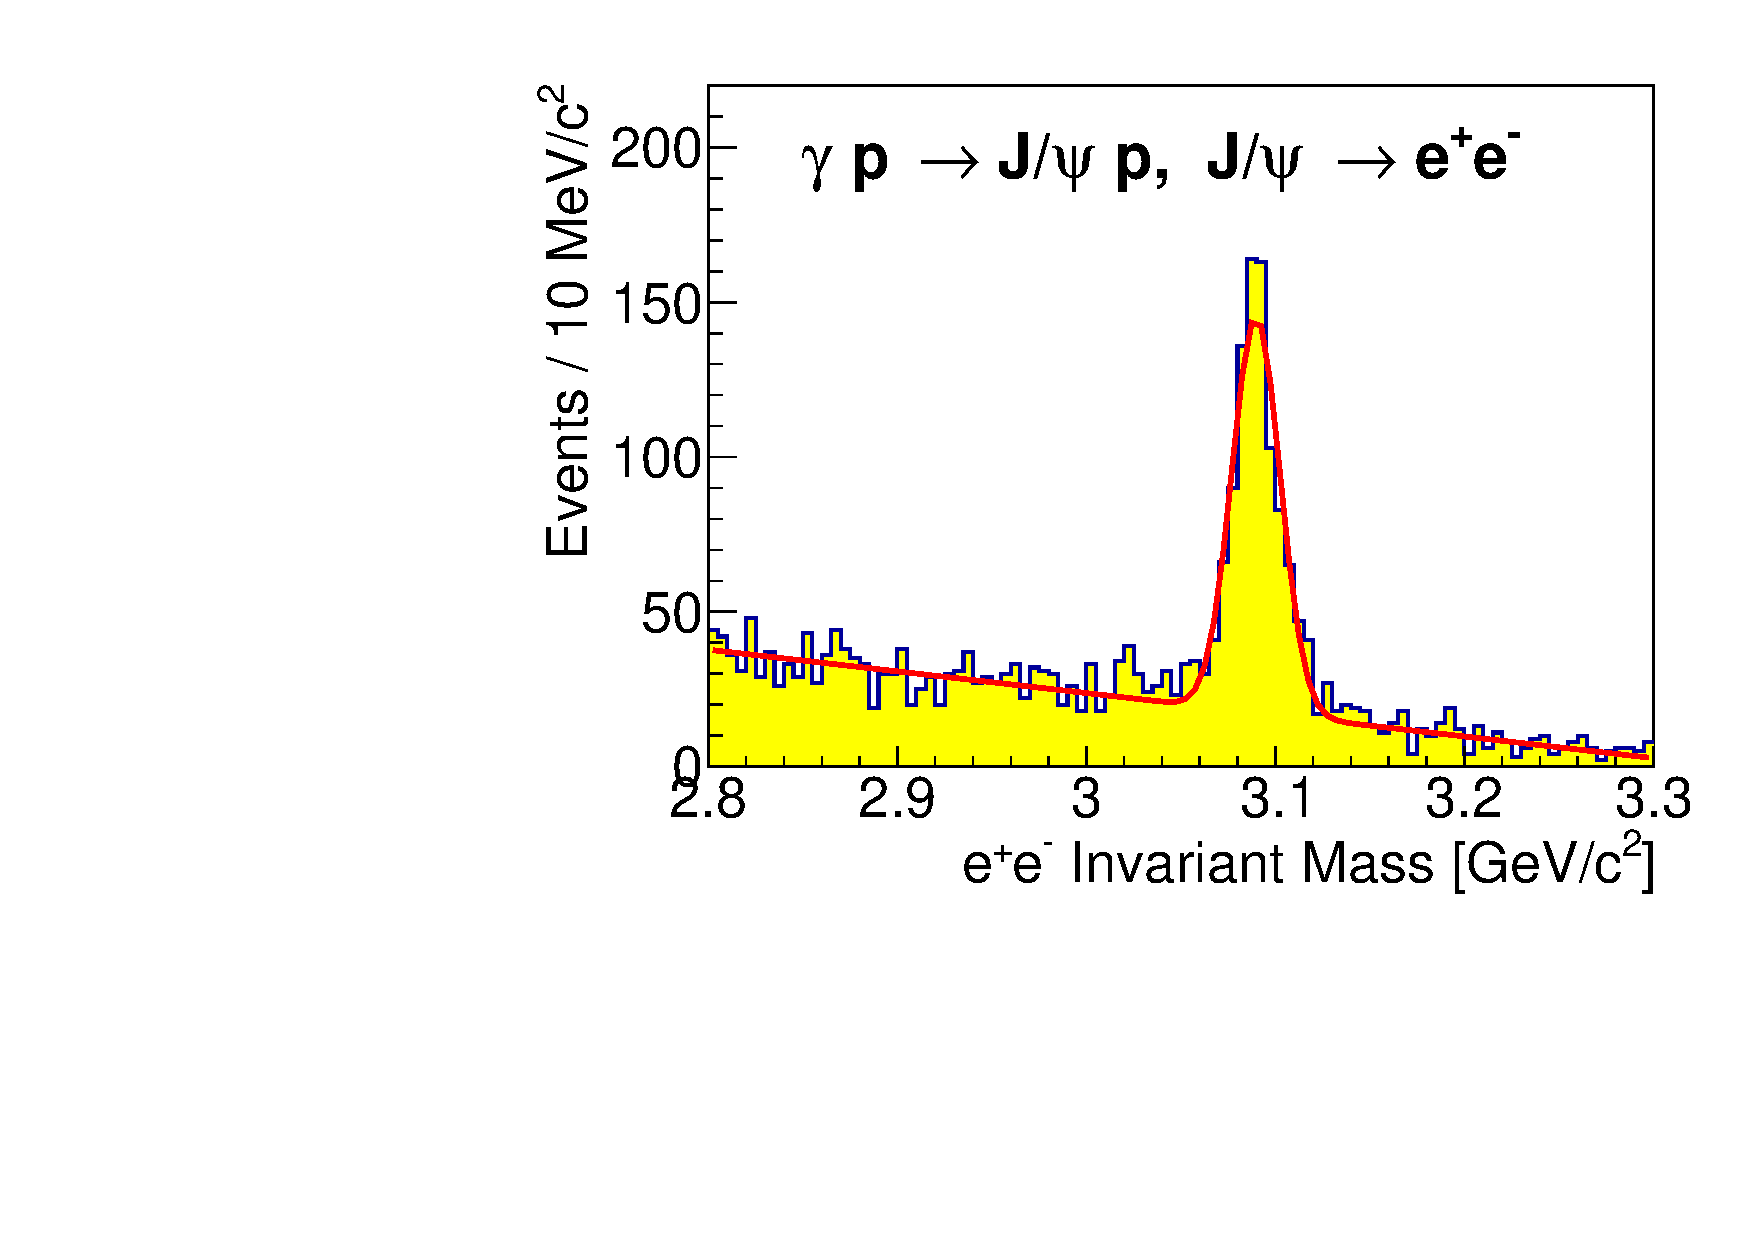
\includegraphics[width=0.42\textwidth]{figures/jpsi_mass.pdf}
\caption{\label{fig:invmass2}
(Left) $\Lambda^0\pi^-$ invariant mass distribution from $\gamma p \to K^+ K^+ \pi^- \pi^- p$. (Right) $e^+e^-$ invariant mass distribution from kinematically fit $\gamma p \to e^+e^- p$ events. (Color online)}
\end{center}
\end{figure}

\subsection{Particle identification \label{sec:perfpid}}

Particle identification in \gx{} uses information from both energy loss in different detector systems and time-of-flight measurements.  This information can be used for identification in several ways.  The simplest method is to apply selections directly on the relevant PID variables.  To include detector resolution information, one can create a $\chi^2$ variable comparing a measured value to the expected value for a particular hypothesis, that is
\begin{equation}
    \chi^2(p) = \left(  \frac{ X(\mathrm{measured}) - X(\mathrm{expected})_p}{\sigma_X} \right)^2
\end{equation}
where $X$ is the given PID variable, $p$ is the particle hypothesis, and $\sigma_X$ is the resolution of this variable.  Multiple PID variables can be combined into one probability, or a figure-of-merit.   Standard, loose selections on time-of-flight and energy loss are sufficient for initial physics analyses, while the performance of more complicated selections is being actively studied.

At sufficiently large $\theta$, the energy loss for charged particles in the central drift chamber $dE/dx$ can be used.   Fig.~\ref{fig:performcdcdedx} illustrates these distributions for positively charged particles, showing a clear separation of pions and protons in the momentum range $\lesssim 1$~GeV. % along with the standard selection used to separate pions and protons.
The $dE/dx$ resolution is approximately 27\%, with the separation between the pion and proton bands dropping from about $8\sigma$ at $p=0.5$~GeV/$c$ to about $2\sigma$ at $p=1.0$~GeV/$c$, with both bands fully merged by $p=1.5$~GeV/$c$.

\begin{figure}[tbp]
\begin{center}
%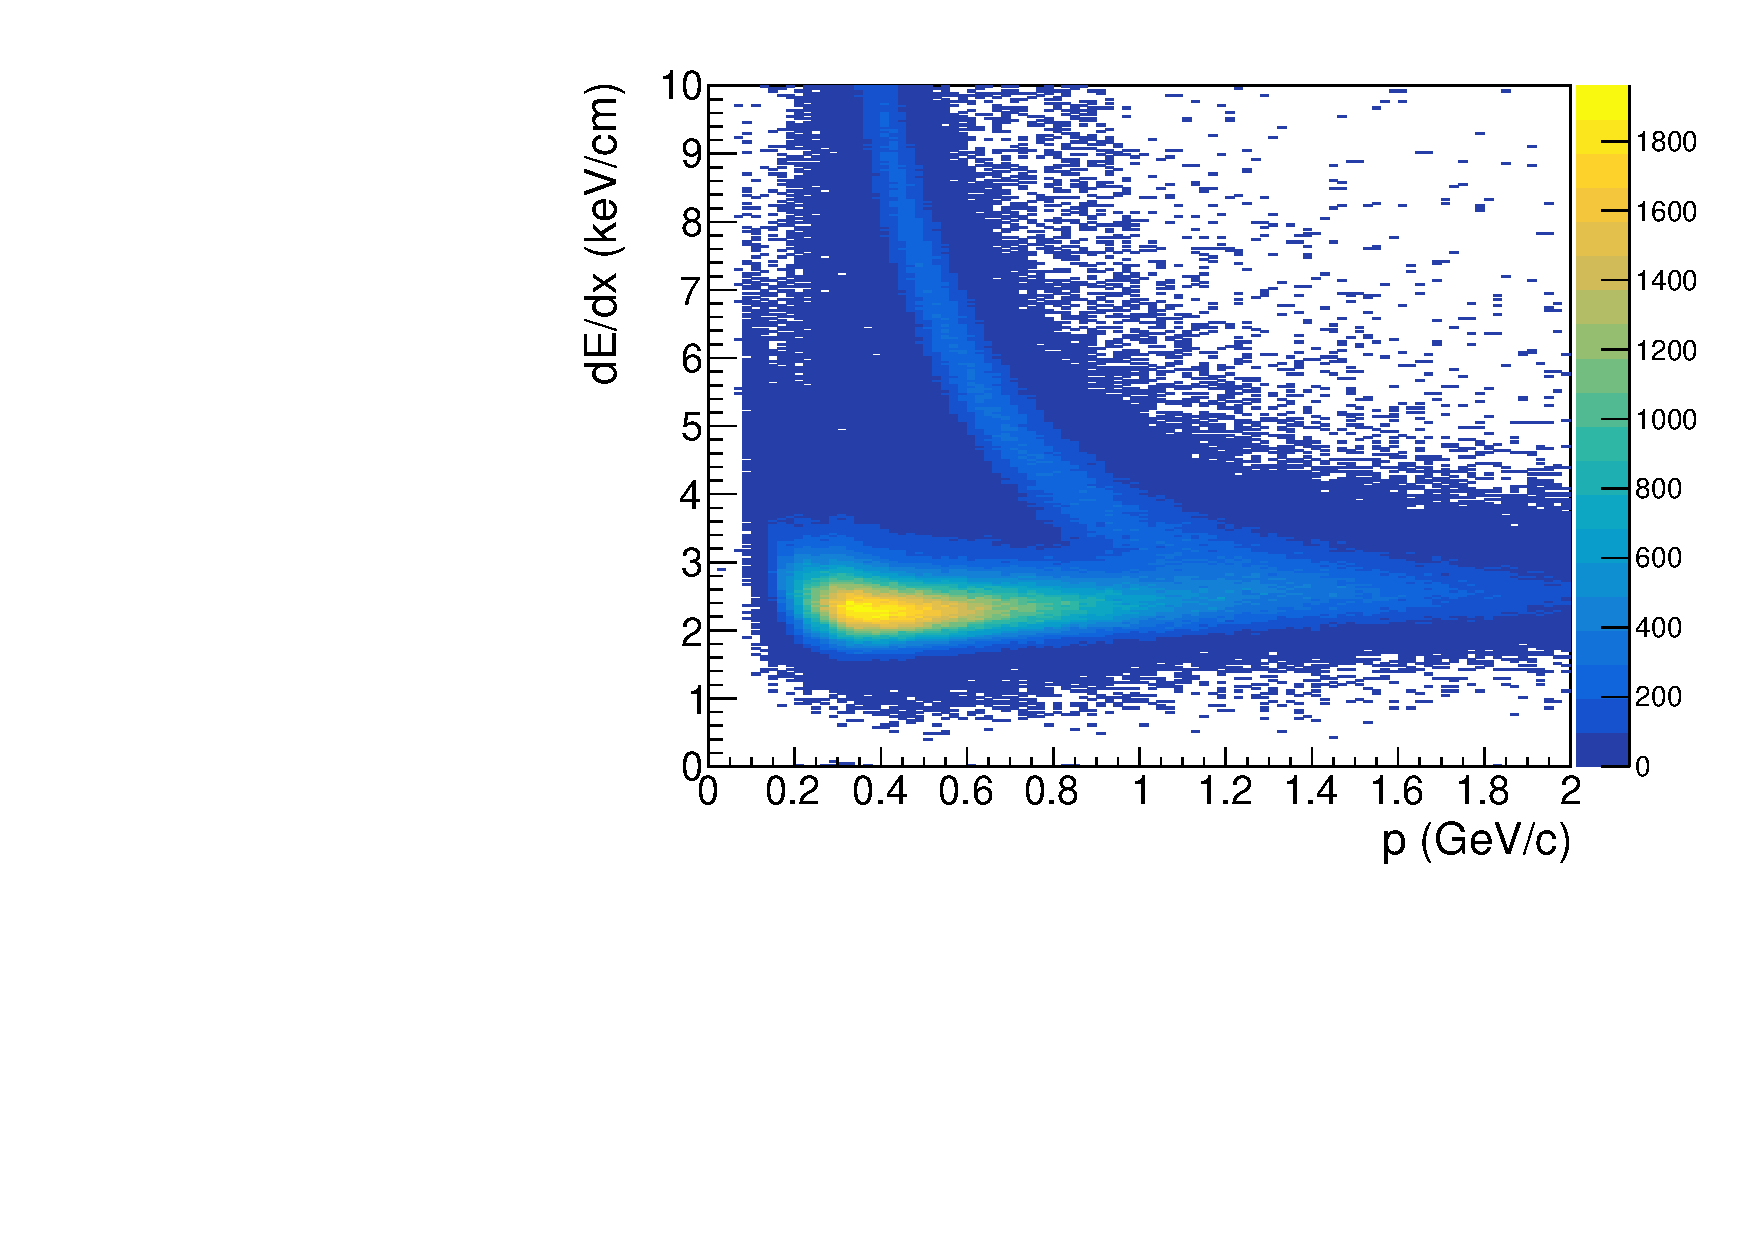
\includegraphics[width=0.6\textwidth]{figures/cdc_pos_dedx.pdf}
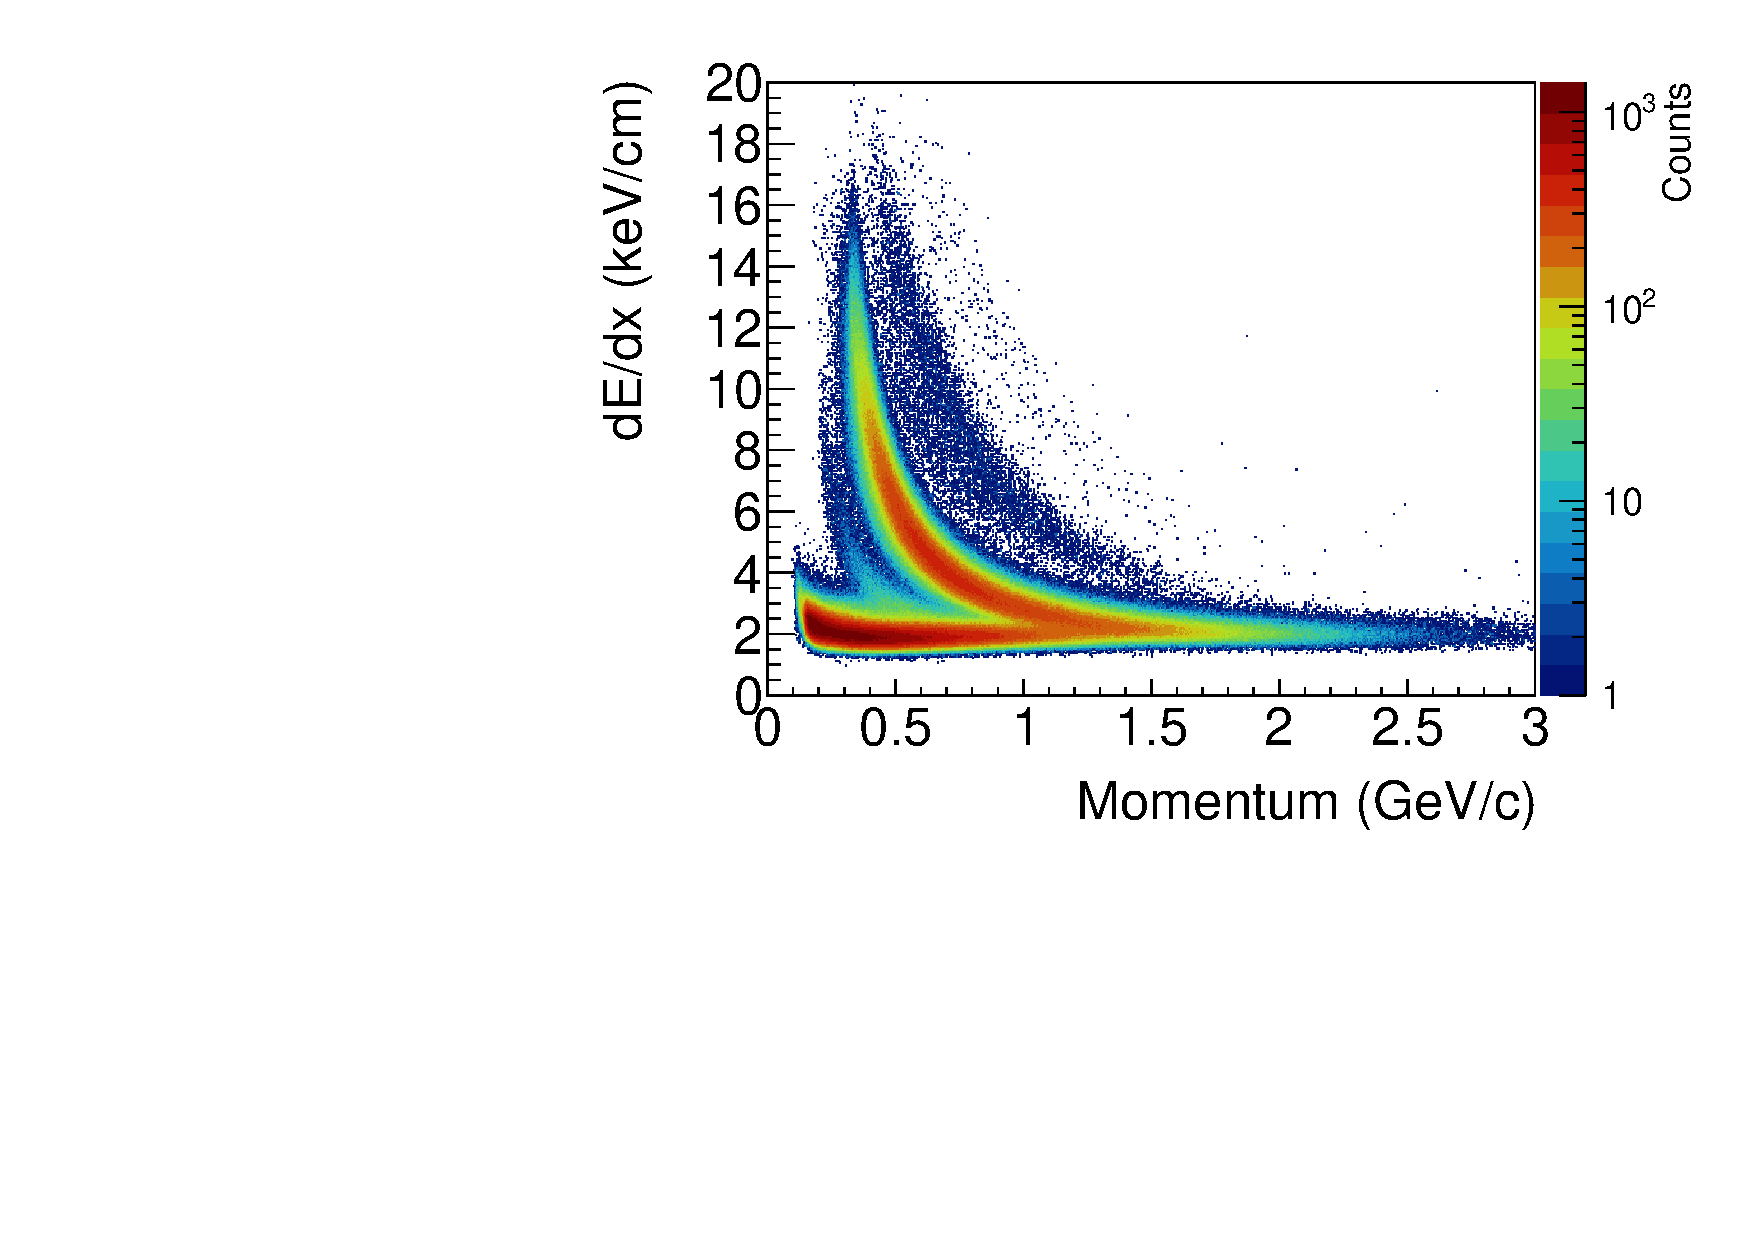
\includegraphics[width=0.6\textwidth]{figures/cdc_dedx.pdf}
\caption{\label{fig:performcdcdedx}
CDC energy loss ($dE/dx$) for positively charged particles that have at least 20 hits in the detector, as a function of measured particle momentum.  The band corresponding to protons curves upwards, showing a larger energy loss than pions and other lighter particles at low momentum.  The two bands show a clear separation for momenta  $\lesssim 1$~GeV.  A faint kaon band can be seen between them.
}
\end{center}
\end{figure}

The primary means of particle identification is through time-of-flight measurements, and information from several sources is combined to make the most accurate determination.  The RF reference signal from the accelerator is used to define the time when each photon bunch enters the target.  The reconstructed final-state particles are used to determine which photon bunch most likely generated the detected reaction, with the primary determination coming from the signals from the Start Counter associated with the charged particle tracks.  The photon bunch determination has a resolution of $<10$~ps. Each charged particle is associated with additional timing information based on the hit in the highest resolution detector (for example the BCAL or TOF).  The flight  time to this measured hit $t_\mathrm{meas}$ relative to the time of the photon bunch that generated the event $t_\mathrm{RF}$ can be used to distinguish between particles of different mass.  Two common variables that are used are the velocity ($\beta$) determined using the measured time-of-flight and the momentum of the particle, and $\Delta t_\mathrm{RF}$, the difference between the measured and RF times after they both have been extrapolated back to the center of the target, assuming some particle-mass hypothesis.
An example of the separation between different particle types can be seen in Fig.~\ref{fig:betavsp}.
The loose selections used for initial analyses of this data placed on the $\Delta t_\mathrm{RF}$ distributions and the momentum dependence of the resolution of this variable in different detectors are shown in Fig.~\ref{fig:timingresol}.  
Requiring reconstructed particles to have  $\Delta t_\mathrm{RF} \lesssim 1-2$~ns has been found to be sufficient for analyses of high-yield channels which are the focus of initial analysis.  The study of the selections required for more demanding channels is ongoing.

\begin{figure}[tbp]
\begin{center}          
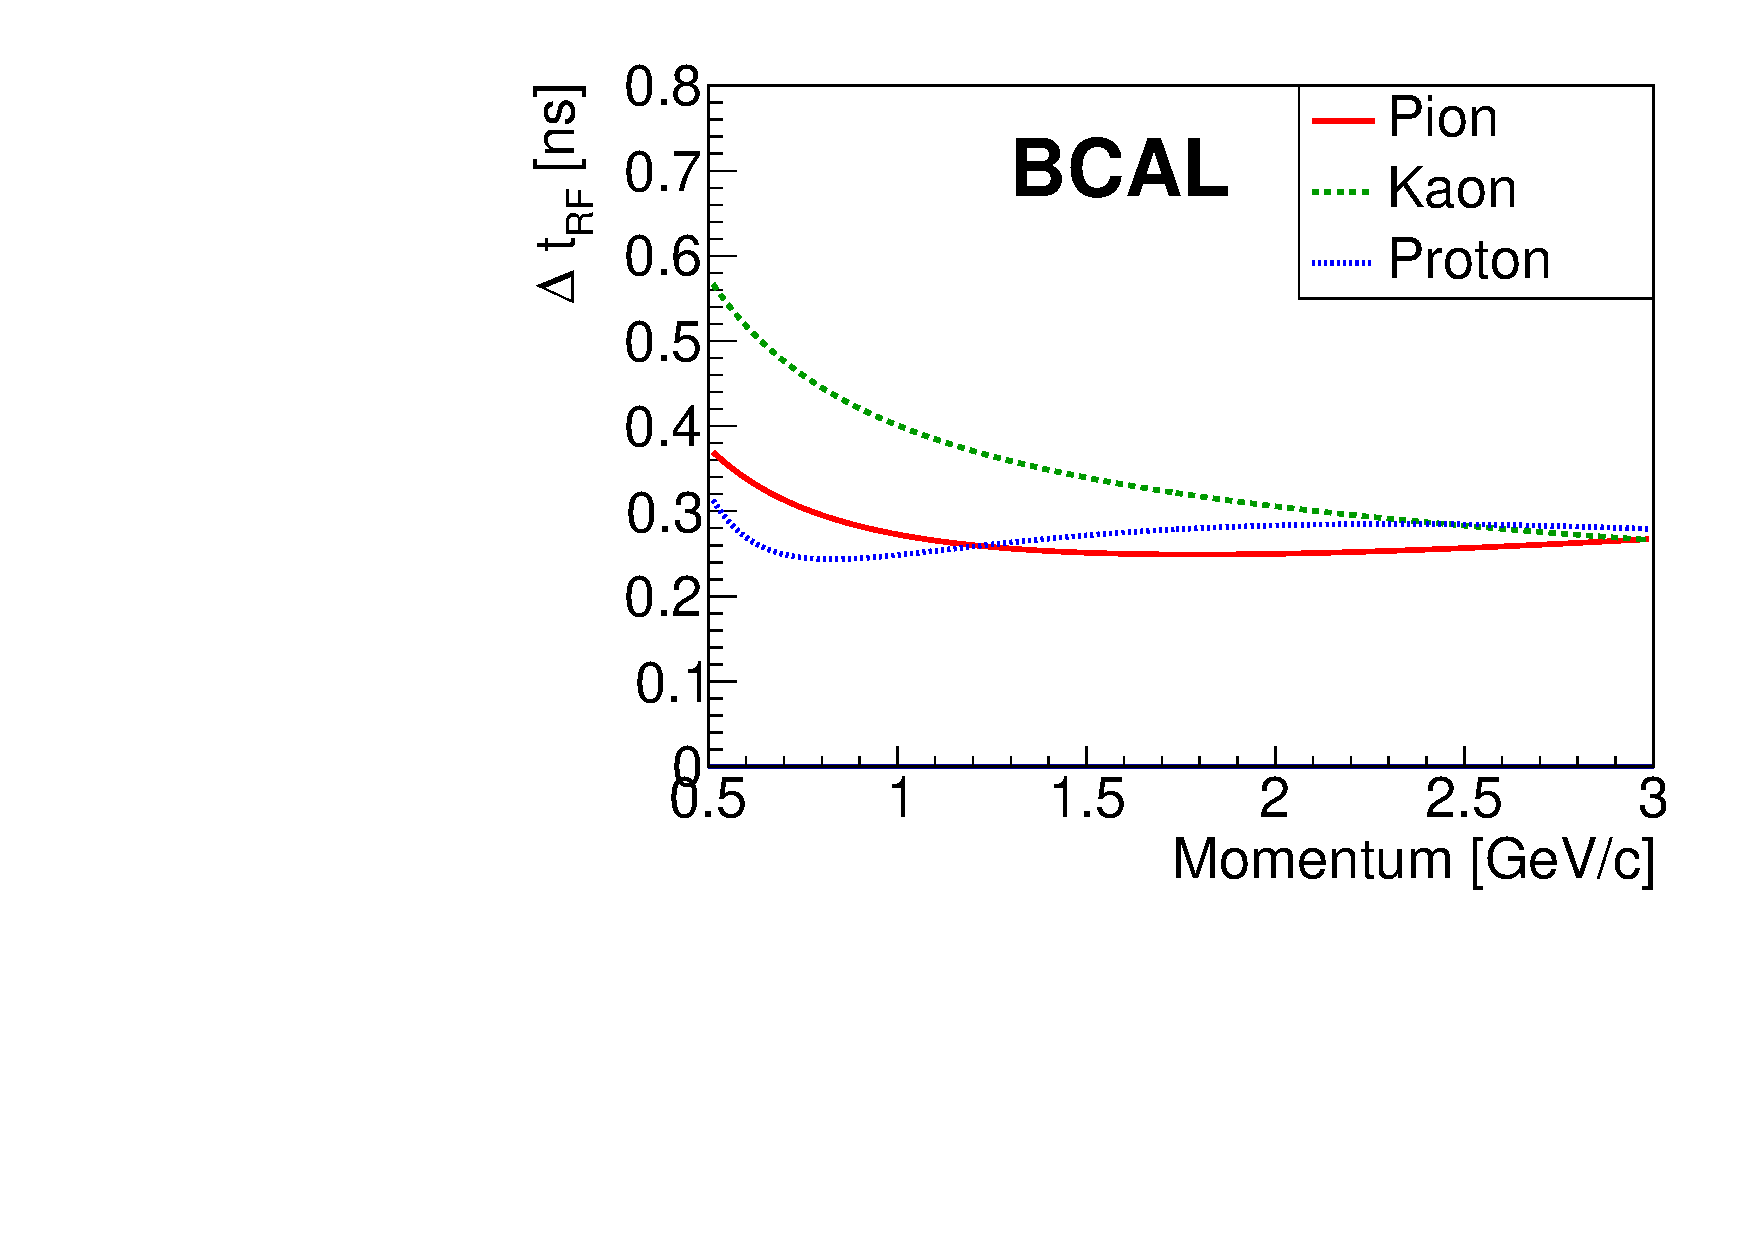
\includegraphics[width=0.29\textwidth]{figures/bcal_deltat_resol.pdf}
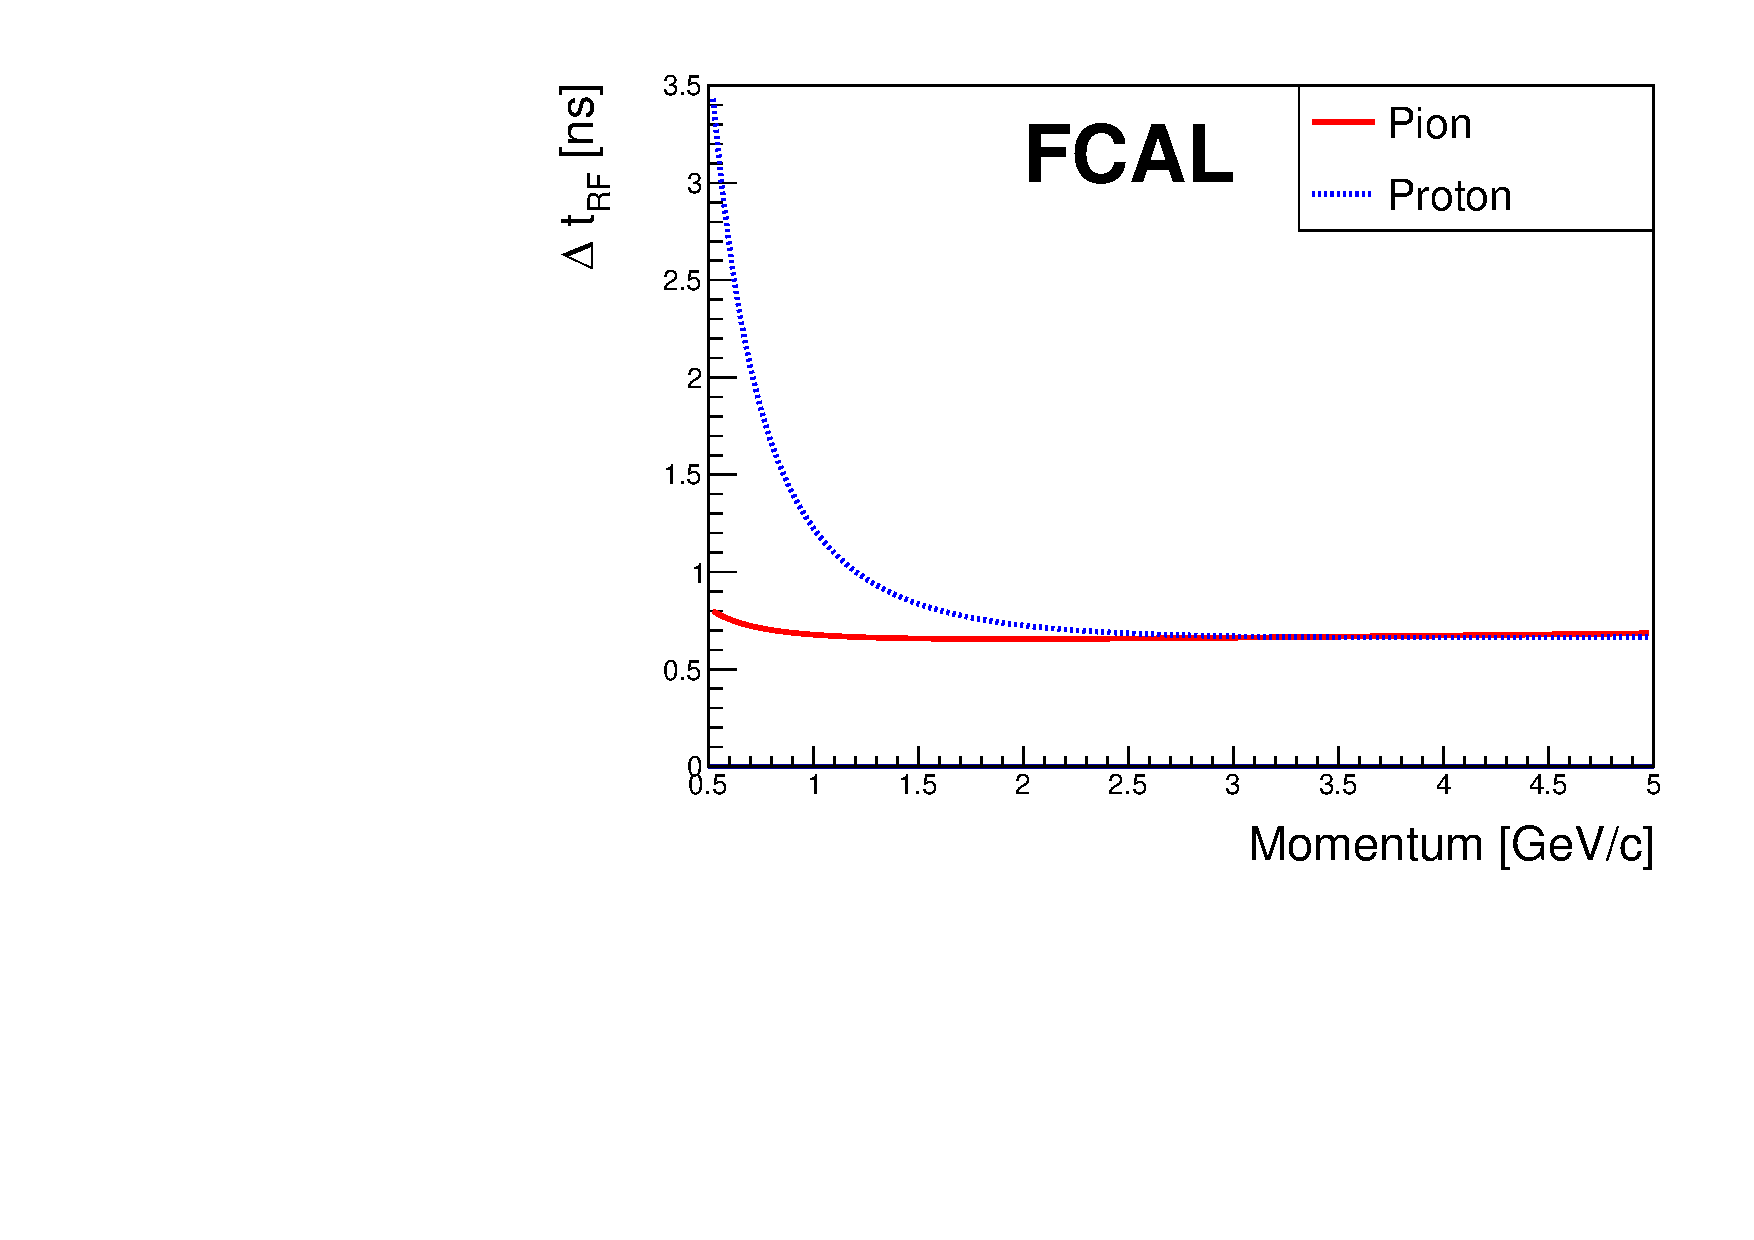
\includegraphics[width=0.29\textwidth]{figures/fcal_deltat_resol.pdf}
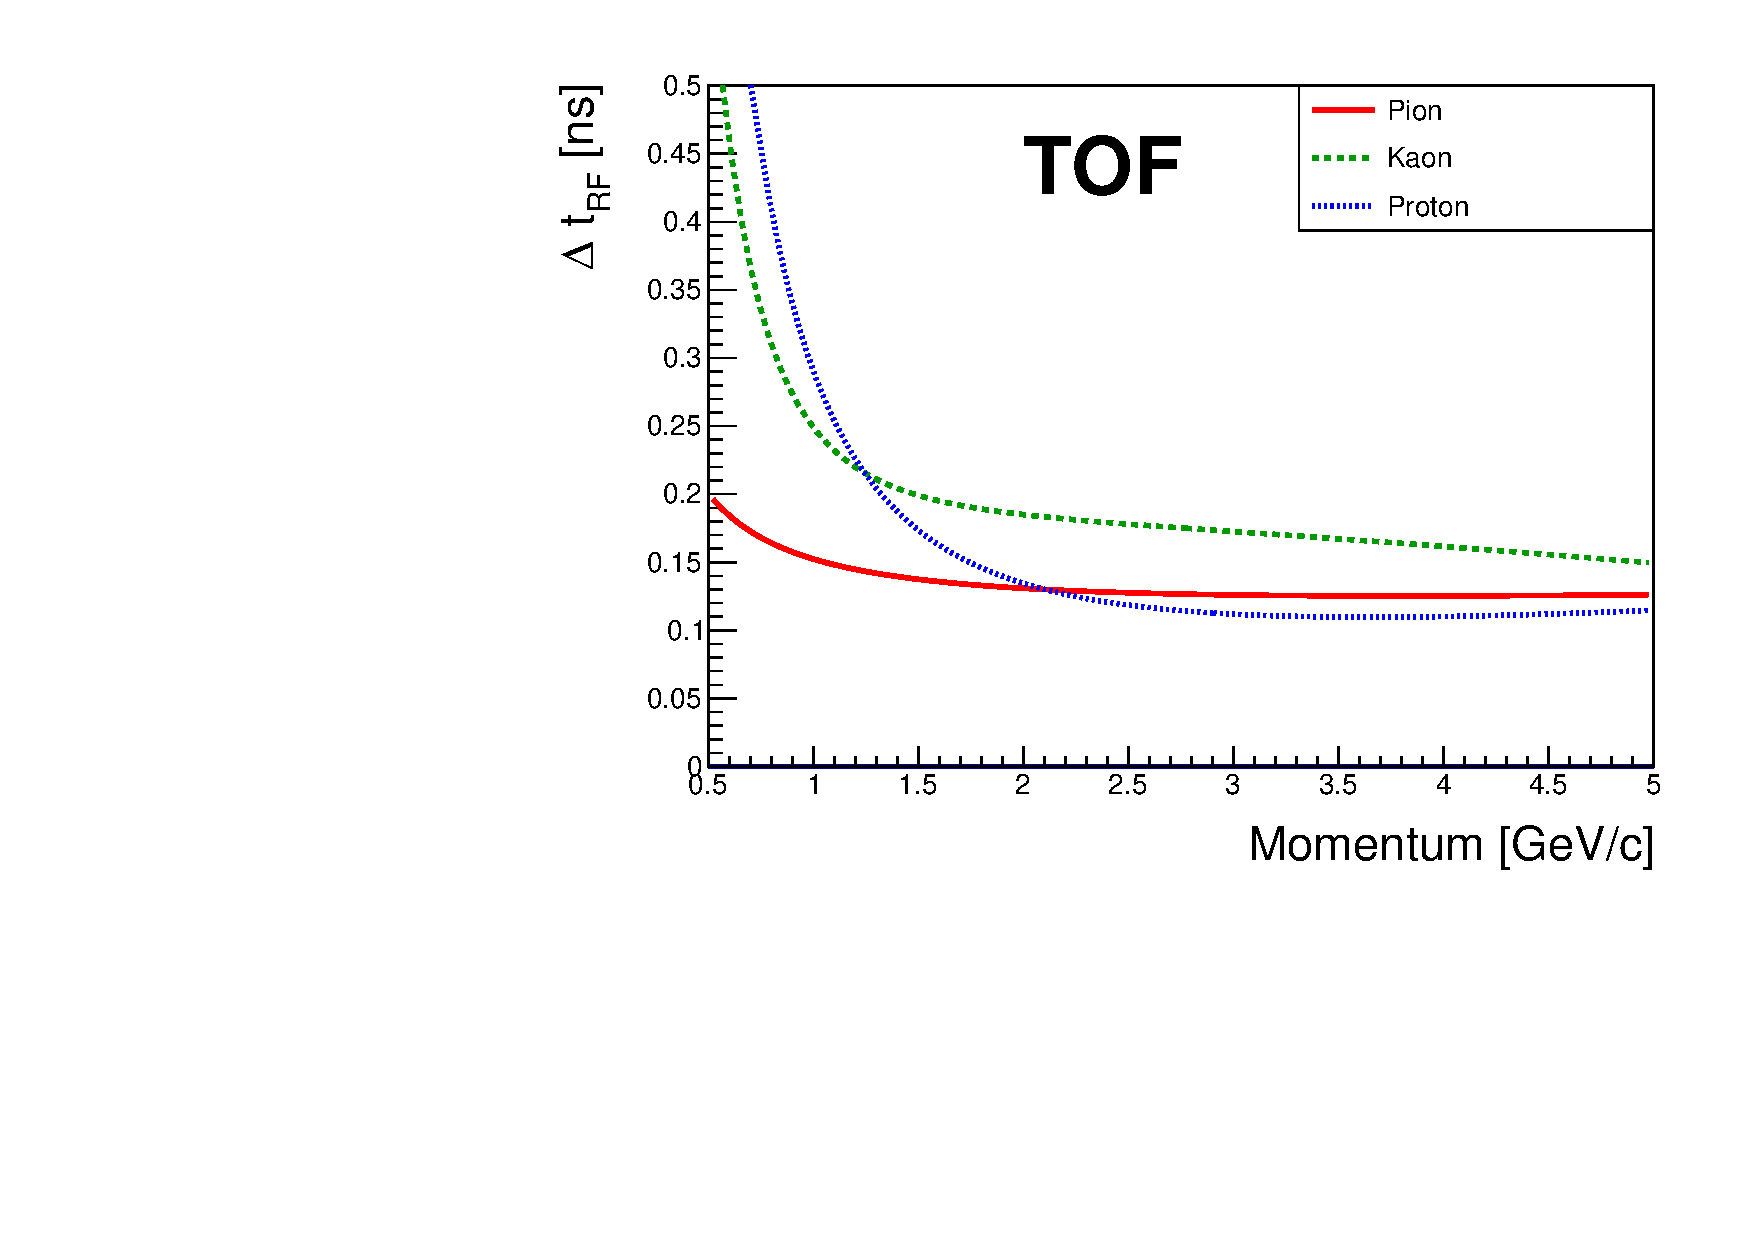
\includegraphics[width=0.29\textwidth]{figures/tof_deltat_resol.pdf}

\caption{\label{fig:timingresol}
Resolution as a function of particle momentum for  $\Delta t_\mathrm{RF}$ in various subdetectors: (left) BCAL, (center) FCAL, (right) TOF
 (Color online)}
\end{center}
\end{figure}


Electrons are identified using the ratio of their energy loss in the electromagnetic calorimeters $E$ to the momentum reconstructed in the drift chambers $p$.  This $E/p$ ratio should be approximately unity for electrons and less for hadrons.  The overall distribution of this variable is illustrated for both calorimeters in  Fig.~\ref{fig:performeop}.  Other variables, such as the shape of the showers generated by the charged particles in the calorimeter, promise to provide additional information to separate electron and hadron showers.

\begin{figure}[tbp]
\begin{center}
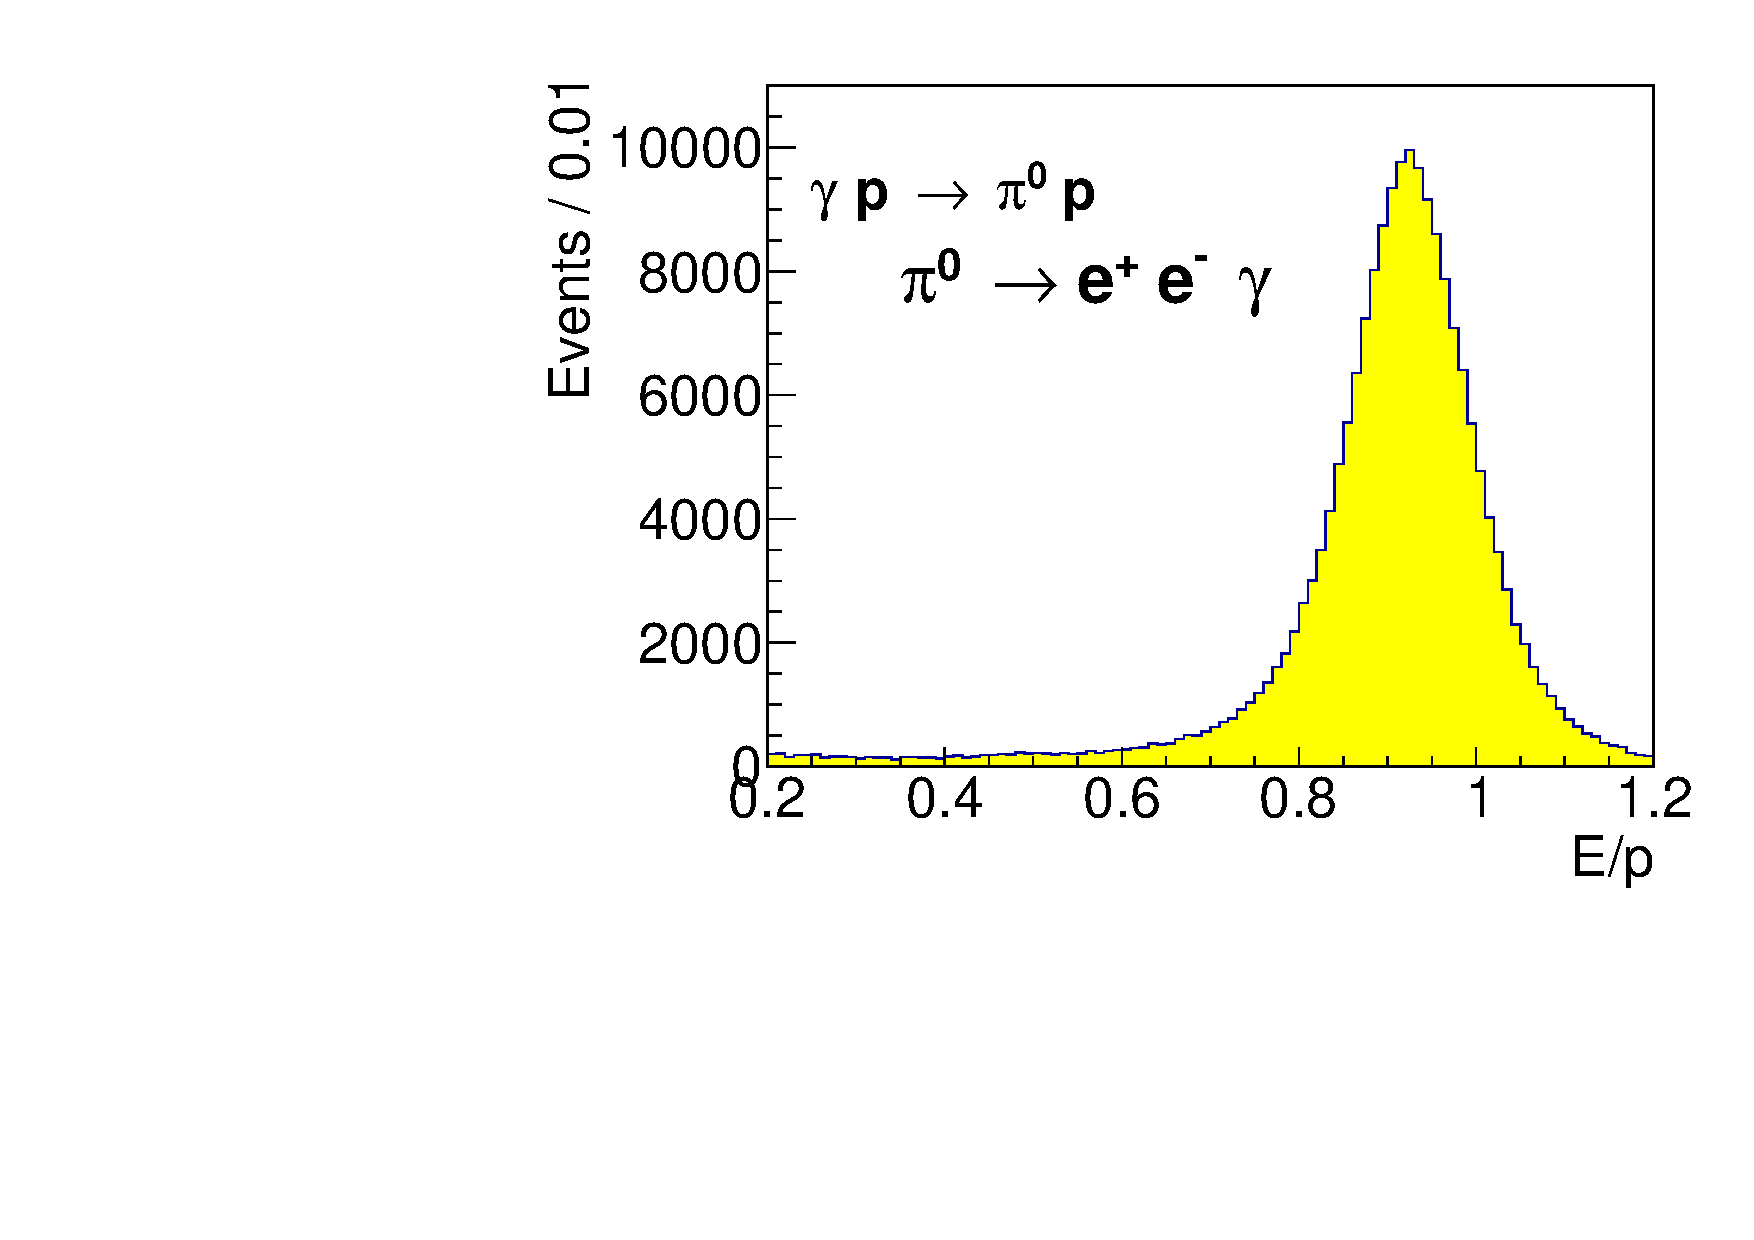
\includegraphics[width=0.4\textwidth]{figures/fcal_ep.pdf}
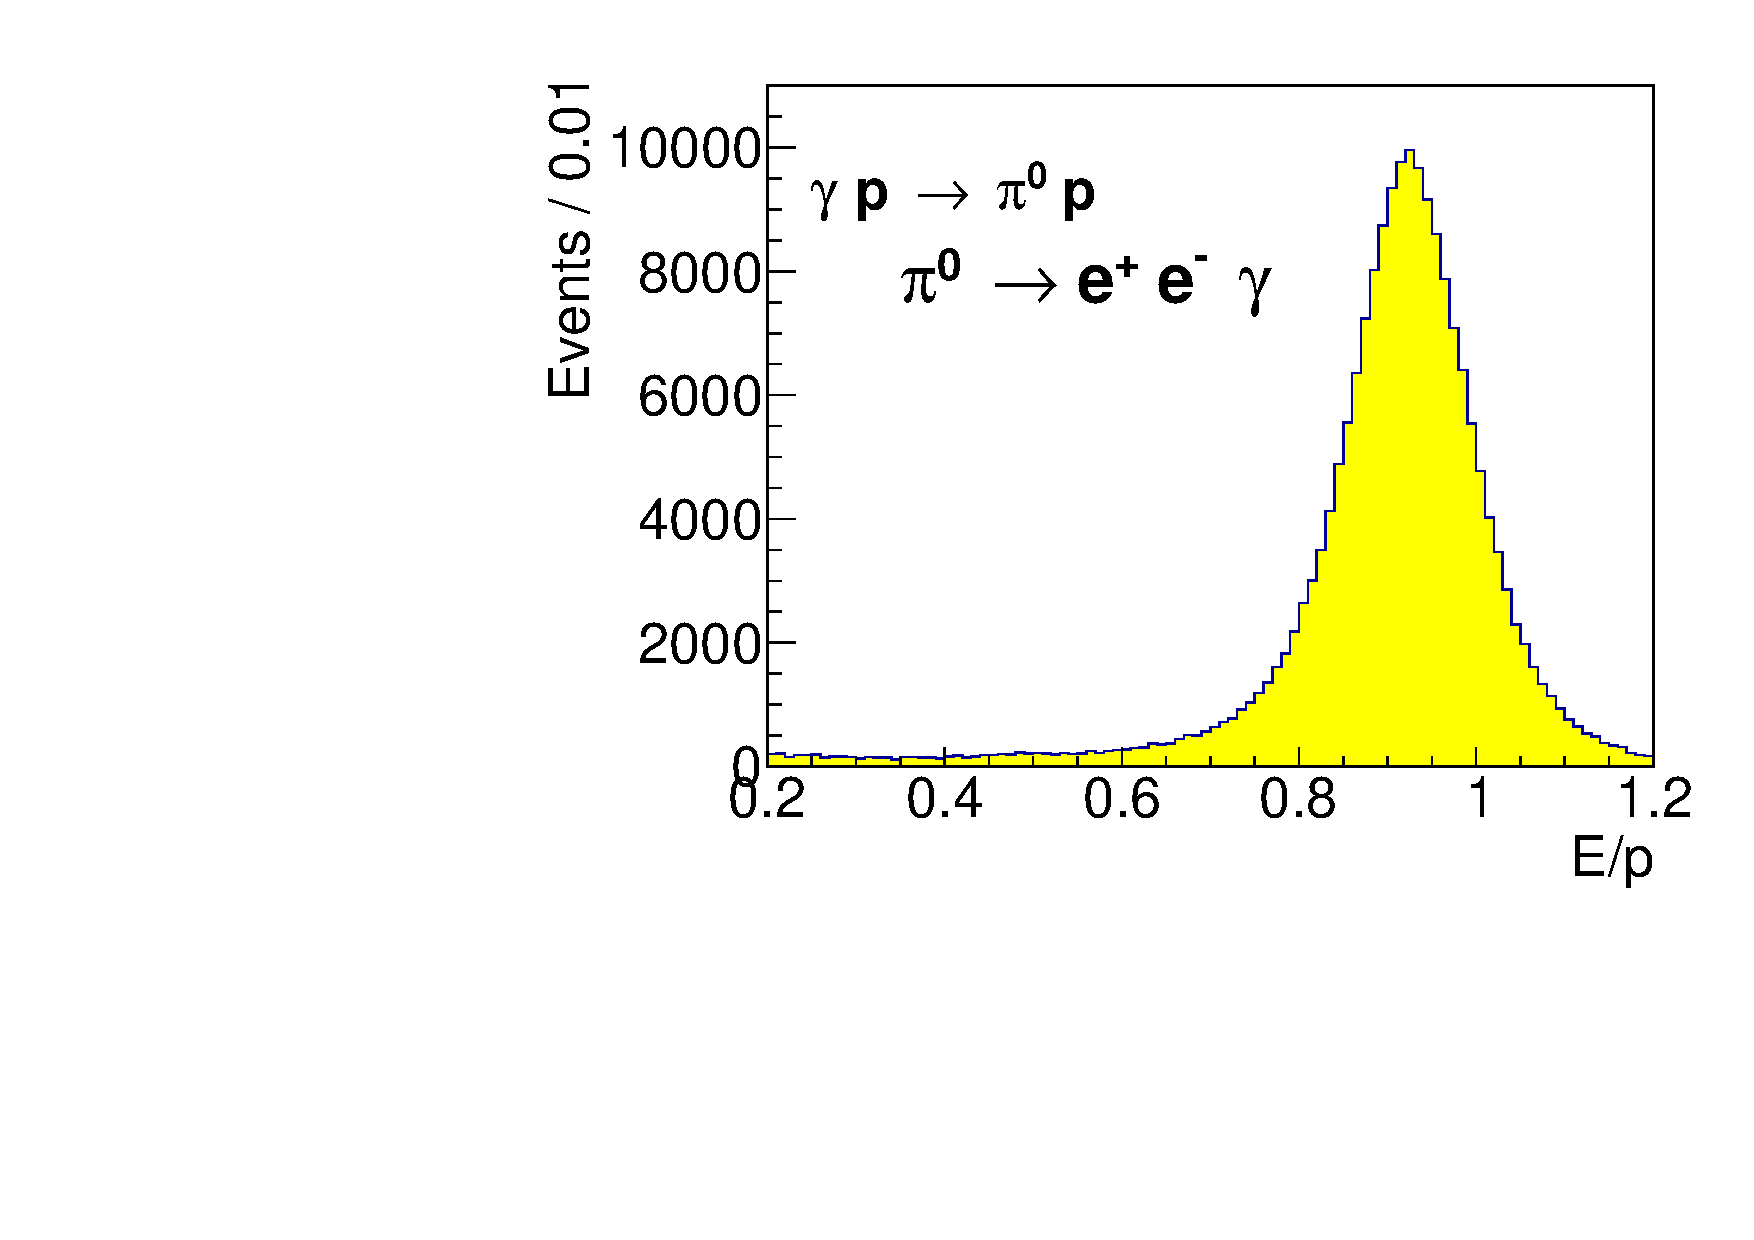
\includegraphics[width=0.4\textwidth]{figures/fcal_ep.pdf}
\caption{\label{fig:performeop}
Electron identification in the calorimeters is performed using the $E/p$ variable, the ratio of the energy loss in the electromagnetic calorimeters ($E$) to the momentum reconstructed in the drift chambers ($p$).  This distribution is shown for selected samples of electrons from (left) $\gamma p \to \pi^0$, $\pi^0 \to e^+e^-\gamma$, where the $e^\pm$ are reconstructed in the FCAL, and (right) ....
}
\end{center}
\end{figure}


%Particle identification and mis-identification rates are summarized in Fig.~X.

%\subsection{Systematic uncertainties \label{sec:systematics}}
